\documentclass[twoside,11pt]{article}

% Any additional packages needed should be included after jmlr2e.
% Note that jmlr2e.sty includes epsfig, amssymb, natbib and graphicx,
% and defines many common macros, such as 'proof' and 'example'.
%
% It also sets the bibliographystyle to plainnat; for more information on
% natbib citation styles, see the natbib documentation, a copy of which
% is archived at http://www.jmlr.org/format/natbib.pdf


% Available options for package jmlr2e are:
%
%   - abbrvbib : use abbrvnat for the bibliography style
%   - nohyperref : do not load the hyperref package
%   - preprint : remove JMLR specific information from the template,
%         useful for example for posting to preprint servers
%
% Example of using the package with custom options:
%
\usepackage{blindtext}
\usepackage[abbrvbib, preprint]{jmlr2e}
%\usepackage{jmlr2e}
% figures
\usepackage{graphicx}
\graphicspath{ {./images/} }
\usepackage{booktabs}
\usepackage[table]{xcolor}

\usepackage{graphicx}
\usepackage{amsmath,amssymb,amsfonts}
\usepackage{xfrac}
\usepackage{tikz}
\usepackage{cases}
%\usetikzlibrary{shapes.symbols}
%\usetikzlibrary{positioning}
\usetikzlibrary{shapes.geometric, arrows, shapes.symbols}
\usepackage{xcolor}
\usepackage[normalem]{ulem}
\usepackage{bm}
\raggedbottom
\usetikzlibrary{calc} 
\usepackage[export]{adjustbox}
%\usepackage{figures}
\usepackage{subfig}
\usepackage{tikz}
\usetikzlibrary{shapes.geometric, arrows, positioning} % Libraries for node shapes, arrows, and relative positioning
\usepackage{float}

\usepackage{lastpage}
\usepackage{comment}
\usepackage{algorithm}
\usepackage{algpseudocode}
\usepackage{tikz}
\usetikzlibrary{fit}
% Uniform square box command
\newcommand*\mybox[1]{\tikz[baseline=(char.base)]{
    \node[shape=rectangle, draw, inner sep=0pt, minimum width=1.35cm, minimum height=0.5cm, align=center] (char) {#1};}}

\newcommand*\mycircle[1]{\tikz[baseline=(char.base)]{\node[shape=circle, draw, thick, dashed, inner sep=1.5pt, minimum size=0.6cm, align=center] (char) {#1};}}

\newcommand\marknode[2]{\tikz[remember picture,baseline=(#1.base)]\node[inner sep=0pt](#1){#2};}

% Definitions of handy macros can go here

\newcommand{\dataset}{{\cal D}}
\newcommand{\fracpartial}[2]{\frac{\partial #1}{\partial  #2}}

\DeclareMathOperator*{\argmax}{arg\!\max}
\DeclareMathOperator*{\argmin}{arg\!\min}

% Define a safe light gray row color; adjust 0.9 -> lighter, 0.85 -> darker
\definecolor{rowgray}{gray}{0.9}

% Convenience macro for green bold entries
\newcommand{\best}[1]{\textbf{\textcolor{green!50!black}{#1}}}

\usepackage[table]{xcolor}   

% Heading arguments are {volume}{year}{pages}{date submitted}{date published}{paper id}{author-full-names}

\jmlrheading{volume}{2022}{1-\pageref{LastPage}}{[2023]; Revised [2023]}{[2023]}{PAPER ID}{Kenric P. Nelson, Igor Oliveira, Amenah AL-Najafi, and Calden Wolka} 

% Short headings should be running head and authors last names
\ShortHeadings{Extreme models using the CVAE}{Nelson, et al.}

\firstpageno{1}

\begin{document}

\title{Stable training of extreme models using the \\ Coupled Variational Autoencoder}

\author{\name Kenric P. Nelson     \email kenric.nelson@photrek.io \\
        \addr Photrek, Inc.\\ 56 Burnham St, Unit 1, \\
        Watertown, MA 02472
        \AND
        \name Igor Oliveira     \email igor.oliveira@photrek.io \\
        \addr Photrek, Inc.\\ 56 Burnham St, Unit 1, \\
        Watertown, MA 02472 \\
        \addr Instituto de F\'isica, Universidade de S\~ao Paulo, \\
        S\~ao Paulo, SP 05314-970, Brazil
        \AND
        \name Amenah AL-Najafi      \email amenah.alnajafi@photrek.io \\
        \addr Photrek, Inc.\\ 56 Burnham St, Unit 1, \\
        Watertown, MA 02472 \\
        \addr Department of Mathematics, University of Kufa, \\
        299G, Najaf, Iraq
        \AND
        \name Calden Wolka      \email cwloka@hmc.edu \\
        \addr Department of Computer Science\\
        Harvey Mudd College \\
        Claremont, CA 91711-5901, USA 
}

\editor{Eddy McEditor}

\maketitle

\begin{abstract}%   <- trailing '%' for backward compatibility of .sty file
\textcolor{red}{update}
Variational Autoencoders have become increasingly popular due to their ability to represent complex data efficiently and as generators of synthetic data. We modify the standard VAE's cost function by generalizing the KL Divergence to enhance sensitivity to outlier risk. This paper describes the Coupled Variational Autoencoder and demonstrates good performance compared to other innovations, particularly for corrupted data.\end{abstract}

\begin{keywords}
  variational autoencoder, coupled statistics, deep learning
\end{keywords}

\section{Introduction}

Generative artificial intelligence learns complex mathematical models through the iterative optimization of cost functions \citep{bengioDeepLearning2017, kingmaIntroductionVariationalAutoencoders2019}. Historically, these models have been built on long-standing statistical methods rooted in the exponential family and Gaussian distributions \citep{amariInformationGeometryIts2016}. From this foundation, Variational Inference (VI) \citep{bleiVariationalInferenceReview2017} emerged as a core methodology, overcoming the complications of learning a true distribution by optimizing the parameters of an approximate one. The key insight of VI is that minimizing the divergence between the true and approximate distribution is equivalent to maximizing the evidence lower bound (ELBO). Functionally, the negative of the ELBO corresponds to the variational free energy \citep{fristonVariationalFreeEnergy2007}, establishing a deep connection between the information theory of AI and thermodynamic models of nature. 

This connection has recently been expanded by Active Inference \citep{parrActiveInferenceFree2022} to model decision-making and action policies. Within the traditional equilibrium thermodynamics framework, the Boltzmann-Gibbs-Shannon (BGS) entropy and the Kullback-Leibler (KL) divergence naturally emerge as the standard cost functions for measuring model accuracy and uncertainty \citep{jaynesInformationTheoryStatistical1957, mackayInformationTheoryInference2003}.

However, the BGS framework relies on the assumption that a system exists in equilibrium and is governed by linear sources of uncertainty. In reality, many natural and human-made systems operate under environments dominated by nonlinear, multiplicative processes. These include climate hazards, hydro-meteorological fluctuations, financial markets, and complex biological ecosystems, such as epidemiological outbreaks and species abundance distributions  \citep{clausetPowerLawDistributionsEmpirical2009, resnickHeavyTailPhenomenaProbabilistic2007, arnoldParetoDistribution2015, pearsonStudentsCollectedPapers1942}. In classical statistical mechanics, systems composed of independent, non-interacting parts naturally form exponential distributions. Yet, when the components of a system interact multiplicatively or share underlying correlations, their probabilities become statistically coupled. This nonlinear coupling slows the decay rate of the distribution, stretching the standard exponential curve into a heavy-tailed shape and increasing the probability of extreme outlier events.

Modeling these non-exponential distributions requires separating uncertainty into two categories: ``known unknowns," represented by a scale parameter (such as the standard deviation in the exponential family), and ``unknown unknowns," represented by the tail-decay shape. These unknown unknowns generally arise from three factors: intrinsic nonlinear fluctuations in the data, limited sample sizes that reduce degrees of freedom, and the practical requirement that a model remain robust to out-of-distribution events. While extreme cases with vanishing scale parameters yield pure power-law \citep{clausetPowerLawDistributionsEmpirical2009} or scale-free models \citep{barabasiScaleFreeNetworksDecade2009}, most phenomena require both a scale and a shape, leading to non-exponential distributions such as the generalized Pareto \citep{arnoldParetoDistribution2015} and Student's t \citep{pearsonStudentsCollectedPapers1942}.

In particular, real-world data often exhibits extreme heavy-tailed behavior, in which the variance, and even the mean, can become undefined or divergent. This is readily observed in the daily log-returns of low-liquidity markets, such as the emerging trade cryptocurrencies and digital assets including Bitcoin, Ethereum, and Solana \citep{szczygielskiOneShapeFits2020, shanaevFittingReturnFitting2021}. Other complex phenomena include hydro-meteorological extremes, turbulent flows, and biological scale-free networks \citep{koutsoyiannisUncertaintyEntropyScaling2005, gisigerScaleInvarianceBiology2001}. Conversely, traditional generative models implicitly assume finite variance and, when faced with extreme data featuring divergent second moments, classical estimators crash or fail to map the true underlying topology, causing standard VI methods to fail \citep{gurbuzbalabanHeavyTailPhenomenonSGD2021}. When applied to such heavy-tailed data, the traditional BGS entropy becomes dominated by the shape of the tail decay, which breaks the fundamental connection between the distribution's scale and its measure of uncertainty \citep{nelsonUniqueUniversalEntropy2026}.

To build machine learning systems capable of robustly learning in extreme environments or datasets, it is necessary to look beyond the classical exponential family. The Rényi and Tsallis entropies, and the Amari $\alpha$-divergence and Wasserstein metric have to date dominated the exploration of cost functions capable of optimizing non-exponential models \citep{kobayashisQVAEDisentangledRepresentation2020,principeInformationTheoreticLearning2010,liRenyiDivergenceVariational2016,amariBackpropagationStochasticGradient1993, tolstikhinWassersteinAutoEncoders2018}.    . Nevertheless these methods are still limited to domains of finite variance \cite{caoCoupledVAEImproved2022}. The $alpha$-divergence function has a discontinuity at $\alpha=1$, which limits its practical utility. The Wasserstein metric has a strong theoretical foundation, but implementations are typically limited to the power 2 case. The Renyi entropy retains the additive information property, while the Tsallis entropy is non-additive. The Tsallis $q$-statistic framework has several misalignments with physical properties that limit its theoretical foundation \citep{nelsonOpenProblemsNonextensive2024}.

Recent breakthroughs in non-equilibrium statistical mechanics have resolved this by demonstrating that the coupled entropy is the unique, universal entropy for complex systems, measuring uncertainty at the informational scale of the maximizing distribution, separating the system's linear scale, the ``known unknowns", from its nonlinear statistical coupling, that is, the ``unknown unknowns" \citep{nelsonUniqueUniversalEntropy2026}. The coupled entropy establishes a delicate balance between the generalized coupled logarithm, which for positive coupling increases the penalty on outliers, and expectations over a modified probability space, the independent-equals distribution, which reduces the outlier samples \citep{al-najafiIndependentApproximatesProvide2026}. The independent-equals expectation acts as a dampener during the training process, ensuring that the training samples have a finite variance that will converge to a computable solution, even when the learned model has undefined variance. Leveraging this unique combination, the coupled entropy can robustly and accurately model extreme heavy-tailed systems.

\textcolor{red}{include the paper sections.}

\section{Background}

The Variational Autoencoder (VAE) \citep{kingmaIntroductionVariationalAutoencoders2019} provides an ideal testbed for validating this framework, as this generative algorithm maps data into a statistical latent space using a Gaussian prior and the free energy loss function. Previous literature has attempted to improve the VAE by modifying its loss function. The $\beta$-VAE \citep{higginsBetavaeLearningBasic2017} introduces a scalar $\beta$ to reweight the KL penalty; however, we show in this paper that this is equivalent to modifying the variance of the Gaussian prior, remaining confined to the exponential family, without adding any new effective parameter. Other approaches utilizing the Rényi and Tsallis entropies \citep{kobayashisQVAEDisentangledRepresentation2020, kobayashiSparseRepresentationLearning2023,liRenyiDivergenceVariational2016, futamiVariationalInferenceBased2018, akramiRobustVariationalAutoencoder2019}, increase sensitivity to tail decay. However, these methods are restricted to shape parameters where the variance is defined.

Recognizing these limitations, some models explicitly introduce heavy-tailed architectures. The $t^3$-VAE \citep{kim$t^3$VariationalAutoencoderLearning2023} incorporates Student's t-distributions and a power divergence metric. While this improves generation in low-density regions, it is restricted to degrees of freedom to $\nu > 2$, enforcing a finite statistical variance and preventing the learning of truly extreme distributions. 

In this paper, we build upon the coupled entropy framework to overcome these limitations by introducing a generalized CVAE architecture that replaces the free energy (KL divergence and log-likelihood reconstruction loss) with the Coupled Free Energy \citep{nelsonUniqueUniversalEntropy2026}. To validate this methodology, we evaluate the model across both standard and extreme datasets. First, we test the CVAE on the CelebA and MNIST image datasets, including corrupted variants, demonstrating improved representation accuracy and robustness to noise compared to traditional Gaussian priors. Second, to test the framework in a truly extreme environment, we apply the CVAE to learn the distributions of daily log-returns for major cryptocurrencies, such as Bitcoin, Ethereum, Solana, Cardano (ADA), Binance Coin (BNB), and Dogecoin, spanning from their inception through late 2025. While the CVAE shows solid structural improvements in image domains, its performance leap is much more pronounced in financial data. Because these cryptocurrency returns inherently exhibit extreme heavy-tailed behavior with divergent variance, standard equilibrium algorithms severely degrade. The CVAE, however, successfully and stably captures these highly volatile distributions, confirming its unique capacity to learn complex systems where classical machine learning fails.

We build on the recent work of \citep{caoCoupledVAEImproved2022}, which extended the traditional VAE framework into a Coupled Variational Autoencoder (CVAE). The original CVAE demonstrated that replacing the standard VAE loss function with one derived from coupled entropy \citep{nelsonAverageUncertaintySystems2017} improves the generation of synthetic data and increases robustness against corruptions. However, early CVAE implementations sampled directly from a heavy-tailed latent distribution, which caused numerical instabilities for larger coupling values due to divergent variance. We advance this foundation by optimizing the coupled free energy using the independent-equals distribution \citep{al-najafiIndependentApproximatesProvide2026, nelsonVariationalInferenceOptimized2025}, ensuring that the training samples maintain a finite variance even when capturing extreme tail risks.

To evaluate this improved mathematical framework, we utilize Convolutional Neural Networks (CNNs) \citep{lecunGradientbasedLearningApplied1998} for both the encoder and decoder. Specifically, our model uses a four-layer convolutional encoder and a four-layer transpose convolutional decoder. We demonstrate that training these convolutional networks with the Coupled Free Energy yields performance gains when generating representations of complex and corrupted datasets. These results confirm that the mathematical benefits of the coupled entropy framework are scalable and applicable across more advanced neural network architectures.

\subsection{Variational Autoencoders}

Given a set of high-dimensional data, such as a library of images, a VAE \citep{kingmaIntroductionVariationalAutoencoders2019} \citep{doerschTutorialVariationalAutoencoders2021} learns a probabilistic model that enables it to generate new samples that mimic the originals. One would like to learn a model $p_\theta\left(\mathbf{z}|\mathbf{x}\right)$ that maps the data $\mathbf{X}$ to a condensed latent variable $\mathbf{Z}$ with parameters $\theta$ learned by an encoder network. Unfortunately,  this turns out to be intractable. Instead an approximate distribution $q_\phi\left(\mathbf{z}|\mathbf{x}\right)$ is learned such that the divergence, $D(p||q)$, is minimized.

\begin{figure}[ht!]
    \centering
    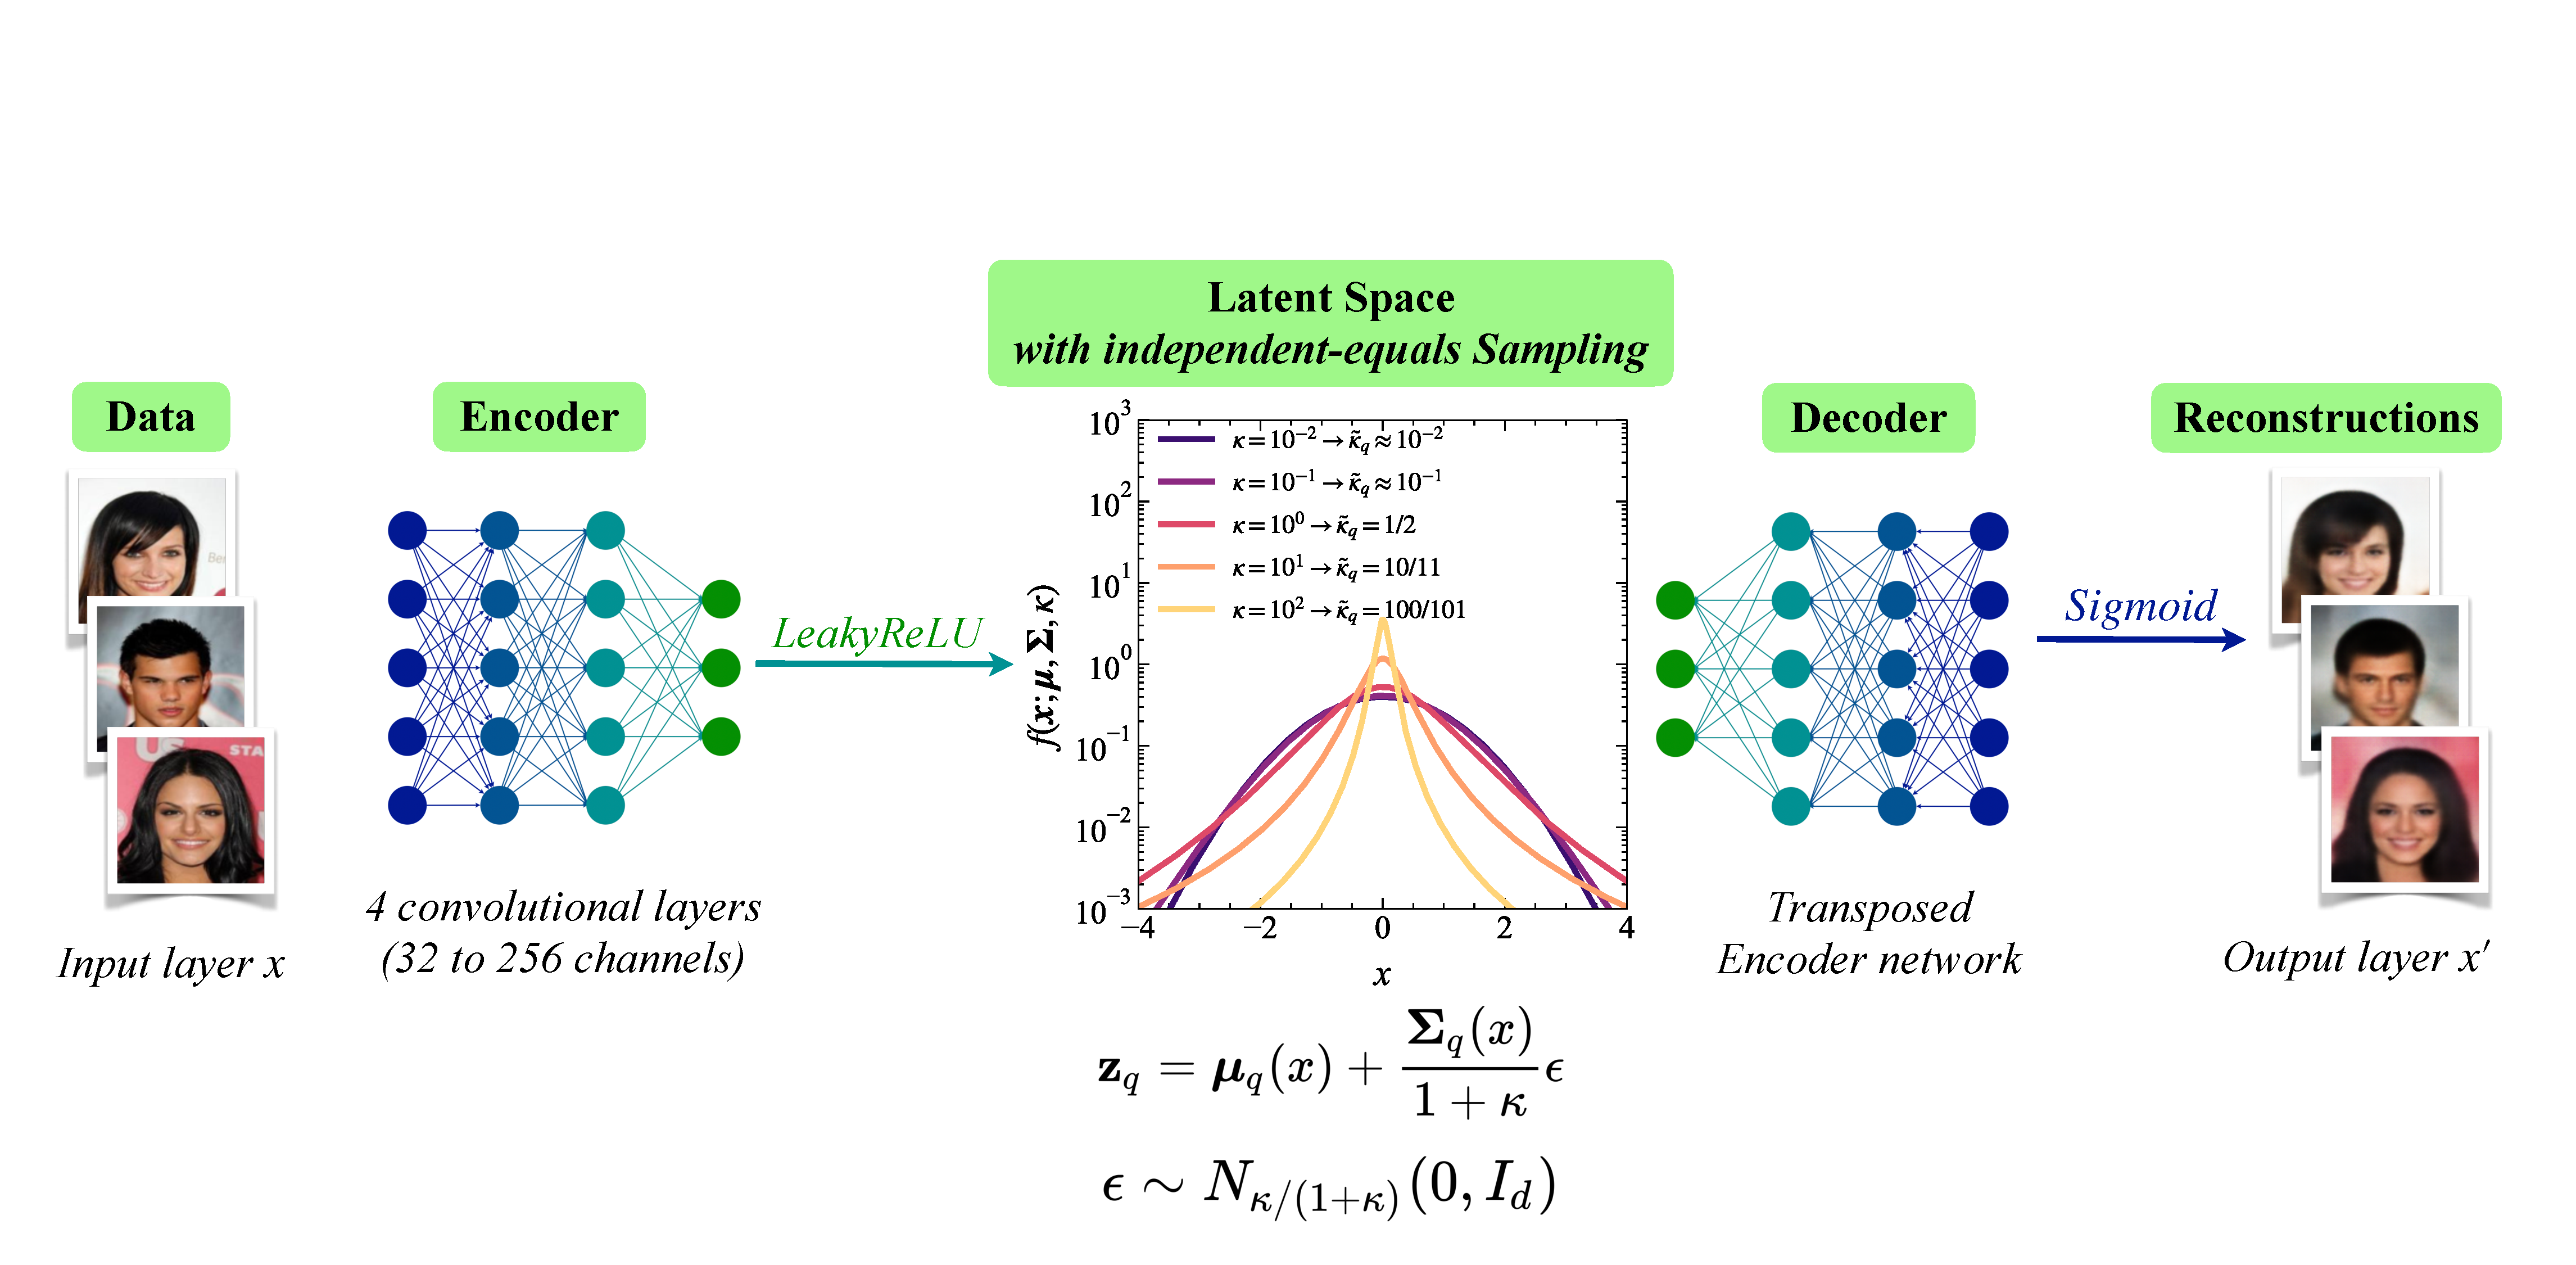
\includegraphics[width=\textwidth]{CVAE_design.pdf}
    \caption{Architecture of the Coupled Variational Autoencoder (CVAE). The neural network processes high-dimensional data (e.g., face images) through an encoder comprised of four convolutional layers, progressively expanding from 32 to 256 channels with LeakyReLU activations to extract hierarchical features. The encoder maps these features to a latent space by outputting the parameters of a Coupled Gaussian distribution: the mean vector $\mu_q(x)$ and the diagonal covariance matrix $\Sigma_q(x)$. The core innovation of the CVAE is the introduction of the independent-equals expectation during the reparameterization step. Rather than sampling directly from the encoded distribution, the model scales the covariance by $\frac{1}{1+\kappa}$ and draws the noise vector $\epsilon$ from an adjusted Coupled Gaussian distribution $\mathcal{N}_{\kappa/(1+\kappa)}(0, I_d)$ with modified nonlinearity $\tilde{\kappa} = \kappa/(1+\kappa) $, ensuring that the latent embedding remains highly stable even at extreme nonlinearities (e.g., $\kappa \gg 1$). Finally, the sampled latent vector $z_q$ is passed through a transposed convolutional decoder, culminating in a Sigmoid activation to yield the final reconstructed image $x^\prime$.}
    \label{fig:cvae_architecture}
\end{figure}

Minimization of the divergence between the desired distribution and the approximation can be shown to be achieved by maximizing an evidence lower bound (ELBO) or equivalently minimizing the free energy (FE). The ELBO includes two components, the likelihood of the data generated by the decoder network, $p_\theta\left(\mathbf{x}|\mathbf{z}\right)$ and the negative of the divergence between the posterior and prior of the latent distribution, $-D\left(q_\phi\left(\mathbf{z}|\mathbf{x}\right)||q(z)\right)$.

\begin{equation}
\begin{split}
    \log p_\theta(\mathbf{x}) 
    &=\mathbb{E}_
    {q_\phi(\mathbf{z|x})}
    \left[\log \left[p_\theta(\mathbf{x})
    \frac{q_\phi(\mathbf{z|x})}{q_\phi(\mathbf{z|x})}\right]\right] \\
    &=\mathbb{E}_
    {q_\phi(\mathbf{z|x})}
    \left[\log \left[\frac{p_\theta(\mathbf{x,z})}{q_\phi(\mathbf{z|x})}
    \frac{q_\phi(\mathbf{z|x})}
    {p_\theta(\mathbf{z|x})}\right]\right] \\
    &=\underbrace{\mathbb{E}_
    {q_\phi(\mathbf{z|x})}
    \left[\log \left[\frac{ p_\theta(\mathbf{x,z})}
    {q_\phi(\mathbf{z|x})}\right]\right]}_
    {\text{ELBO}}+ \underbrace{\mathbb{E}_{q_\phi(\mathbf{z|x})}
    \left[\log \left[\frac{q_\phi(\mathbf{z|x})}
    { p_\theta(\mathbf{z|x})}\right]\right]}_
    {\text{Divergence}}
\end{split}
\end{equation}
The expression in the first line adds canceling terms of the posterior distribution of the latent variable $z$ given the data $x$. Rearranging those terms shows that the marginal log-likelihood of the data can be expressed as the ELBO plus the divergence between the model $q_\phi$ and the actual distribution $p_\theta$. Thus, minimizing the divergence is achieved by maximizing the ELBO. The ELBO is equivalent to the negative free energy \citep{fristonFreeEnergyPrinciple2006}, thus connecting the methodology with physical principles and neuroscience models.

However, maximizing the ELBO assumes that the expected log-average of the model and actual distribution (divergence) is the right thing to optimize. In fact, many problems require optimization of something other than average performance. Often, the worst-case performance or the performance variance also needs to be controlled. Before introducing heavy-tailed distributions to capture extreme data, we first examine standard modifications to the VAE objective, beginning with the reweighting of the divergence term in the $\beta$-VAE. Next, we will introduce the Coupled VAE, which generalizes the ELBO to incorporate relative risk aversion. In doing so, we can train a VAE and potentially other ML algorithms with a controllable sensitivity to outliers in their performance.

\subsection[The beta-VAE is equivalent to modified prior]{The $\boldsymbol{\beta}-$VAE is equivalent to a modifying prior and posterior}

A common modification to the standard VAE objective is the $\beta$-VAE \citep{higginsBetavaeLearningBasic2017}, which scales the Kullback--Leibler divergence term in the evidence lower bound by a hyperparameter $\beta$. Increasing $\beta > 1$ forces the learned posterior distribution to adhere more closely to an independent prior, encouraging simpler and more factorized latent representations \citep{burgessUnderstandingDisentangling$beta$VAE2018}.

However, scaling the divergence weight does not alter the underlying family of distributions. As derived in Lemma~\ref{lemma:beta_prior_equivalence} (Appendix A), adjusting $\beta$ in a standard Gaussian VAE is equivalent to rescaling the variance of the Gaussian prior according to $\sigma_p^2 \approx 1/\sqrt{\beta}$, alongside a corresponding shift in posterior sampling. Rather than introducing new statistical parameters or heavier tails, the $\beta$-VAE remains confined within the standard exponential family.

\begin{figure}[ht!]
	\begin{center}
		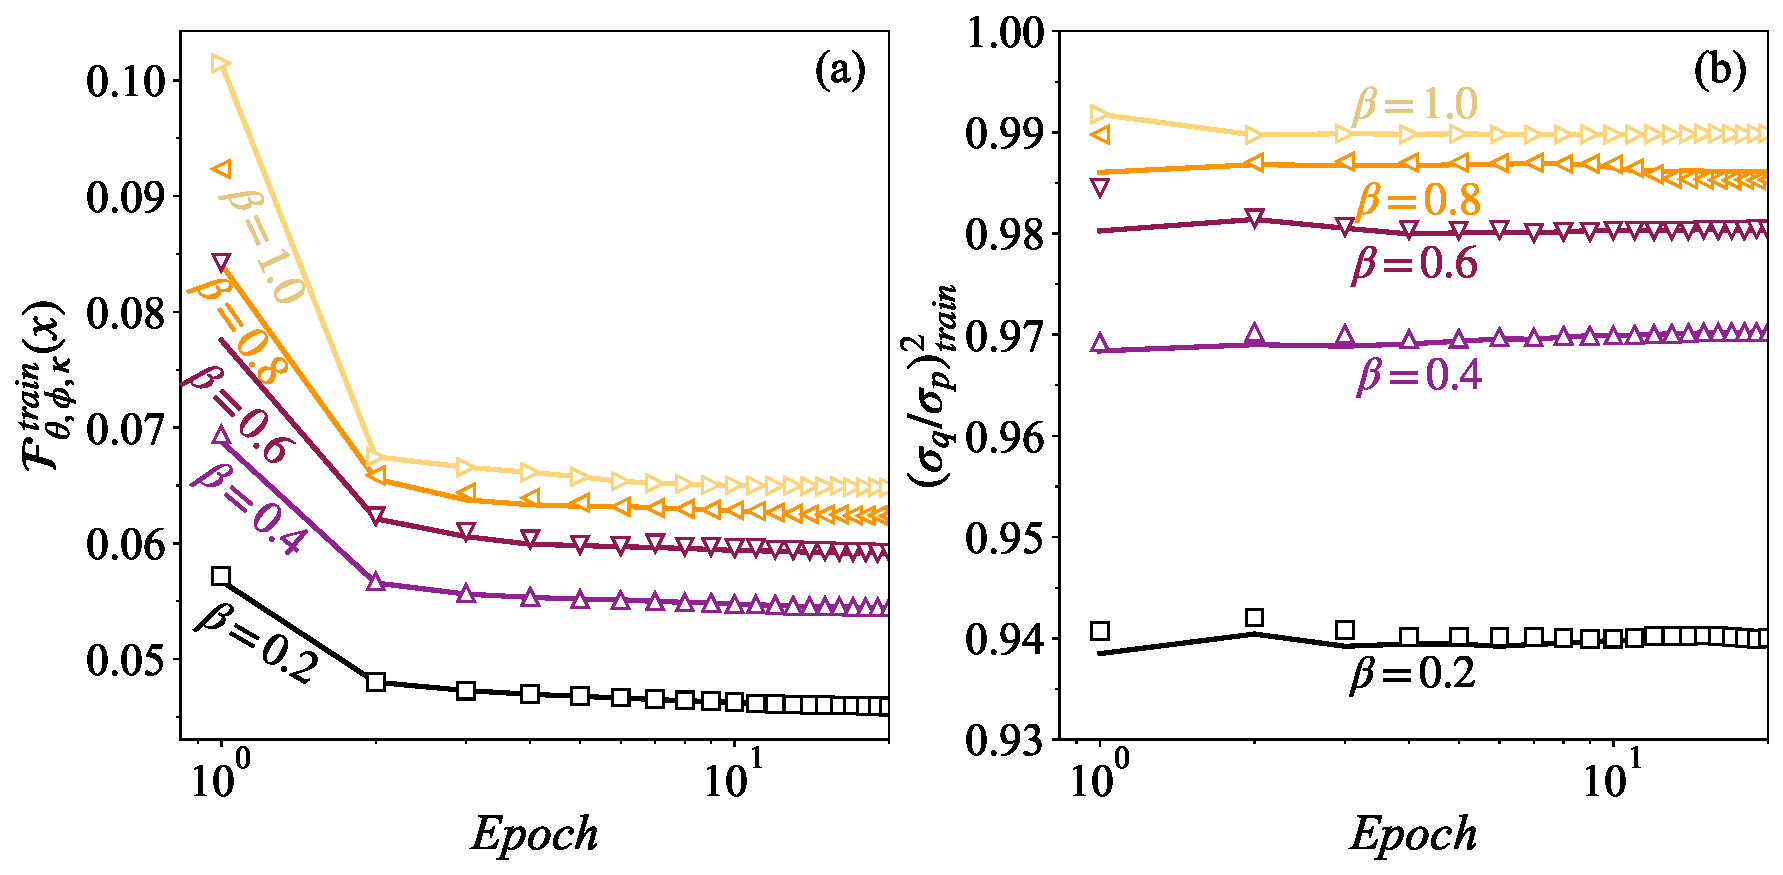
\includegraphics[width= \linewidth]{Beta_epoch_data.pdf} 
		\caption{Comparison between the standard ($\kappa = 0$) $\beta$-VAE with unit prior variance and the standard VAE with adjusted prior variance $\sigma_p^2 = 1/\sqrt{\beta}$. Both (a) the training free energy and (b) the ratio between posterior and prior variance match closely across training epochs.}
		\label{Fig_beta_epochs.png}
	\end{center}
\end{figure}

We validate this relationship experimentally in Figure~\ref{Fig_beta_epochs.png}, tracking the free energy and the variance ratio across training epochs. The numerical results confirm that adjusting the prior variance reproduces the behavior of the $\beta$-VAE. Figure~\ref{Fig_beta_stationary.png} shows the stationary values after 20 epochs across multiple values of $\beta$, confirming that altering $\beta$ acts primarily as a hyperparameter for prior variance tuning rather than a structural change to tail risk. Because tuning $\beta$ merely rescales Gaussian variance without changing the shape of the distribution tails, modeling systems with extreme outliers requires stepping outside the standard exponential family.

\begin{figure}[ht!]
    \centering
    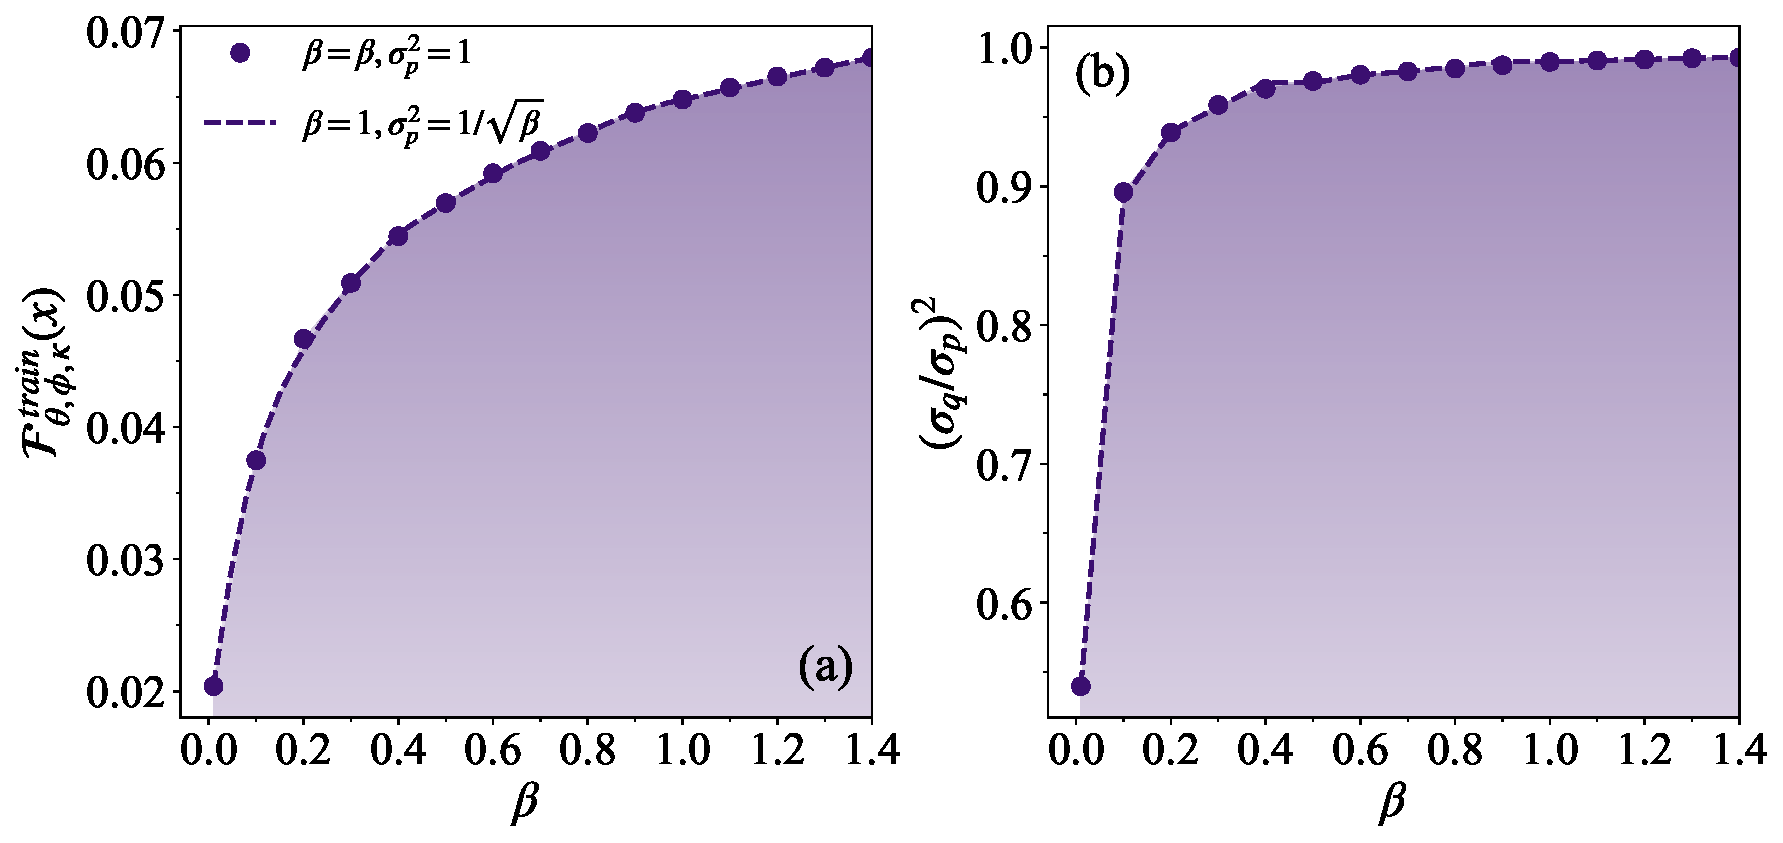
\includegraphics[width= \linewidth]{Beta_stationary_data.pdf} 
    \caption{Stationary metrics after 20 training epochs comparing the $\beta$-VAE with unit prior variance against the standard VAE with adjusted prior variance $\sigma_p^2 = 1/\sqrt{\beta}$. The stationary free energy (a) and variance ratio (b) confirm the mathematical equivalence across choices of $\beta$.}
    \label{Fig_beta_stationary.png}
\end{figure}

\subsection{Generalized VAE designs utilizing complex systems theory}
Recent advances in generative modeling for heavy-tailed data have been replacing standard Gaussian assumptions and KL divergence based regularization with tail-robust alternatives. For instance, the $t^3-$Variational Autoencoder \citep{kim$t^3$VariationalAutoencoderLearning2023} uses a multivariate Student’s t latent distribution \citep{abiriVariationalAutoencodersStudents2019,tippingVariationalInferenceStudentt2005} and replaces the KL divergence with a $\gamma$-power divergence \citep{eguchiPowerDivergence2025} which is closely related to the Amari \citep{amariInformationGeometryIts2016, regliAlphaBetaDivergenceVariational2018} information geometry. Similar systems have been generalizations of the VAE have been developed using the Rényi \citep{liRenyiDivergenceVariational2016} and Tsallis entropy \citep{kobayashisQVAEDisentangledRepresentation2020, kobayashiSparseRepresentationLearning2023} functions.  In related research, heavy-tailed diffusion models generalize diffusion and flow frameworks by introducing Student-t priors, tailored perturbation kernels, and the $\gamma$-divergence objective, yielding controllable tail generation with minimal changes to standard pipelines \citep{pandeyHeavyTailedDiffusionModels2024}. 

These approaches enable computationally tractable mechanisms to learn from heavy-tailed distributions, supporting generative modeling beyond the Gaussian paradigm while preserving training stability. However, a key limitation is that these formulations assume that the degrees of freedom satisfy $\nu>2$, corresponding to the finite-variance regime. On the other hand, comprehensive review studies have shown that real-world data, such as cryptocurrency daily log-returns, often have infinite theoretical variance, that is, an undefined second moment, and in some cases, they yield even an undefined mean or first moment \citep{shanaevFittingReturnFitting2021, szczygielskiOneShapeFits2020}. 

In this report, we report on a significant advance in the architecture of the Coupled Variational Autoencoder (CVAE) \citep{caoCoupledVAEImproved2022, chenUseStudentsTDistribution2020}. The original CVAE designs was similar to the methods using a Student's t latent distribution objective and a generalized free energy in that it allowed for training of models within the domain of well-defined means. The new architecture for the CVAE \citep{nelsonVariationalInferenceOptimized2025} utilizes an expectation over the independent-equals latent distribution, which assures that the training samples have finite variance even as the nonlinear statistical coupling of the latent distribution goes to infinity.  This capability is a unique capability of coupled entropy function \citep{nelsonUniqueUniversalEntropy2026}, which separates the nonlinear and linear sources of uncertainty.  Our method enables more precise risk engines that accurately capture tail-risk events, such as emerging markets, catastrophic losses. More broadly, the methods will be applicable in predictive coding and active inference designs in which inference is completed at individual nodes with limited data.

\subsection{Information Theory for Nonlinear Systems}

While information theory and its physical counterpart, statistical mechanics, establish a broad foundation, there are assumptions built around equilibrium dynamics and the exponential family that are broken in nonlinear, non-equilibrium environments. For instance, temperature is a scale property that fluctuates and therefore becomes difficult to define in nonlinear systems. Likewise, the uncertainty measured by entropy can become so dominated by these nonlinear fluctuations that the uncertainty due to linear sources in the system are overwhelmed. Thus, there has been a long-standing research objective to generalize information theory and statistical mechanics for nonlinear, non-equilibrium systems, which are characterized by non-exponential distributions. The first substantial initiative in this domain was the Rényi entropy \citep{renyiMeasuresEntropyInformation1961, bashkirovRenyiEntropyStatistical2006} which showed that the generalized mean of probabilities could replace the geometric mean used in the BGS entropy, thereby compensating for the effect of non-exponential tail decay. Sharma and Mittel \citep{sharmaNewNonadditiveMeasures1975, nielsenClosedformExpressionSharma2012} proposed a general expression for non-additive entropies. \cite{tsallisPossibleGeneralizationBoltzmannGibbs1988} proposed a non-additive entropy in conjunction with constraints based on the probabilities raised to a power, $p_i^q$; however, the $q$ has since been shown to be a function of more fundamental parameters, and the proposed inverse-scale parameter $\beta$ has been shown to not be the inverse of the scale \cite{nelsonOpenProblemsNonextensive2024}. 

Recently, a new proof \citep{nelsonUniqueUniversalEntropy2026} has clarified that a generalized entropy function must be a measure of the uncertainty at the scale of the generalized Pareto, Student's t, and related shape-scale distributions. The only function that fulfills this requirement is the coupled entropy \citep{nelsonReducedPerplexitySimplified2020, nelsonAverageUncertaintySystems2017}, specified by the nonlinear statistical coupling parameter\footnote{The definition of the nonlinear statistical coupling parameter has evolved as clarity regarding the separation of the nonlinearity from other physical properties has improved. The 2010 paper introducing the topic included an expression called the "source of nonlinearity" which was  confirmed in 2026 as the correct definition. Papers between 2015-25 used a definition equal to the asymptotic tail shape; however, the source of nonlinearity is in fact the shape divided by stretching parameter.} \citep{nelsonNonlinearStatisticalCoupling2010} and composed of two components. The first component is the coupled logarithm, which increases (decreases) the penalty of low probability events for positive (negative) nonlinear statistical coupling. The second component is taking the expectation over the independent equals distribution rather than the distribution being measured. The independent-equals distribution reduces (increases) the sampling of rare events for positive (negative) nonlinearity. The combination is a precise metric that assures accuracy in the tail uncertainty while not becoming unstable.

The nonlinear statistical coupling \citep{nelsonNonlinearStatisticalCoupling2010}, $(\kappa)$ quantifies the source of nonlinearity creating fluctuations and non-exponential characteristics. It's role in defining nonlinearity is explicit in the definition of the coupled logarithm,
\begin{equation} \label{coupledLog}
    a\ln_\kappa x=\ln_{\sfrac{\kappa}{a}} x^a\equiv
    \left\{\begin{matrix}\begin{matrix}
        \frac{a}{\kappa}\left(x^{\kappa}-1\right) & \kappa \neq 0 \\
        a\ln x & \kappa=0
    \end{matrix}
    & x>0,
    \end{matrix}\right.
\end{equation}
where $a$ is an additional power term often associated with the shape of distribution near its location parameter. The inverse is the coupled exponential, 
\begin{equation}
    \exp_{\kappa}\left(\frac{x}{a}\right) = 
    \exp_{\sfrac{\kappa}{a}}^a(x)
    \equiv\left\{ \begin{matrix}
     (1+\kappa \frac{x}{a})_+^\frac{1}{\kappa} & 
     \kappa \neq 0, (b)_+ \equiv \max(0,b) \\
     \exp\left(\frac{x}{a}\right) &
     \kappa=0.
    \end{matrix}\right.
\end{equation}
The foundational connection of these functions to nonlinear systems is via the solution to the nonlinear differential equation:
\begin{align}
y &=  \exp_\kappa^{-1}(x)
= (1+\kappa x)^{-\frac{1}{\kappa}}\\
\frac{dy}{dx}&= -\exp_\kappa^{-(1+\kappa)}(x)=
-\left(1+\kappa x\right)^{-\frac{1}{\kappa}-1}.\\
\frac{d^n}{dx^n}=&(-1)^n\kappa^n\prod_{m=0}^{n-1}\left(\frac{1}{\kappa}+m\right)(1+\kappa x)^{-\frac{1}{\kappa}-n}\\
&= (-1)^n\kappa^n\frac{\left(\frac{1}{\kappa}+n-1\right)!}{\left(\frac{1}{\kappa}-1\right)!}(1+\kappa x)^{-\frac{1}{\kappa}-n}\\
&= (-1)^n\kappa^n\frac{\left(\frac{1}{\kappa}+n-1\right)!}{\left(\frac{1}{\kappa}-1\right)!}\exp_\kappa^{-(1+n\kappa)}(x).
\end{align}
Therefore, for non-integer values the $n$th derivative can be written as

\[
\frac{d^n}{dx^n}(1+\kappa x)^{-\frac{1}{\kappa}}
=(-1)^n\kappa^n\frac{\Gamma\!\left(\frac{1}{\kappa}+n\right)}{\Gamma\!\left(\frac{1}{\kappa}\right)}(1+\kappa x)^{-\frac{1}{\kappa}-n}.
\]

Equivalently,

\[
\frac{d^n}{dx^n}(1+\kappa x)^{-\frac{1}{\kappa}}
=(-1)^n\kappa^n\frac{\displaystyle\int_0^\infty
t^{\frac{1}{\kappa}+n-1} e^{-t}\,dt}{\displaystyle
\int_0^\infty t^{\frac{1}{\kappa}-1} e^{-t}\,dt
}(1+\kappa x)^{-\frac{1}{\kappa}-n}.
\]
%\begin{align}
%    \frac{\text{d}^ny}{dx^n} &= -y^{1+n\kappa} \\
%    y &= \exp_\kappa^{-1}(x) \\
%    \frac{\text{d}y}{dx} &= - \exp_\kappa^{-(1+\kappa)}(x) \\
%    \frac{\text{d}^ny}{dx^n} &= (-1)^{n}(\frac{1}{\kappa}+n-1)!\kappa^n(1+\kappa x)^{-\frac{1}{\kappa}-n} \\
%    &= (-1)^{n}(\frac{1}{\kappa}+n-1)!\kappa^n\exp_\kappa^{-(1+n\kappa)}(x).
%\end{align}
This differential relationship with the exponent $1+n\kappa$ is also essential to the relationship between the survival function and the probability density function for the coupled exponential family of distributions.  The reciprocal of the coupled exponential is the survival function (sf) (one minus the cumulative distribution function (cdf)) of the generalized Pareto distribution, $S\left(x;\mu,\sigma,\kappa\right)\equiv\left(\exp_\kappa{\left(\frac{x-\mu}{\sigma}\right)}\right)^{-1}$, where $\mu$ is the location and $\sigma>0$ is the scale. Importantly, this definition is required to assure that the scale and nonlinear statistical coupling are independent. This can be generalized further to include the Student's t distribution, which has a power of two for the argument of the coupled exponential, and is referred to as the coupled Gaussian distribution. The \textit{coupled distribution} defines a family of heavy-tailed ($\kappa>0$) and compact-support ($-\frac{1}{d}<\kappa<0$) that generalizes the exponential family ($\kappa=0$). On a log-log plot the survival function of the coupled distribution has a slope of $-\frac{1}{\kappa}$  and the the log-log slope of the probability density function (pdf) at the scale, $\sigma$ is minus one. For the coupled variational autoencoder the pdf of the multivariate coupled Gaussian\footnote{For algebraic simplicity the variable $\mathbf{x}$ is treated as a continuous vector variable although these will typically be quantized values in implementation. While $f(\mathbf{x})$ is used to define the pdf, $p(\mathbf{x})$ and $q(\mathbf{x})$ will be used for the VAE definitions in order to be consistent with the literature.}
%\begin{align}
    %f\left(\mathbf{x};\boldsymbol{\mu},\boldsymbol{\Sigma},\kappa\right)
    %&\equiv\left\{\begin{matrix}
    %\frac{1}{Z\left(\boldsymbol{\Sigma},\kappa\right)}
    %\left(1+\kappa\left(\mathbf{x}-\boldsymbol{\mu}\right)^{\intercal}\mathbf{\Sigma}^{-1}\left(\mathbf{x}-\boldsymbol{\mu}\right)\right)_+^{-\frac{1+d\kappa}{2\kappa}}&\kappa\neq0  \\
    %\frac{1}{Z\left(\boldsymbol{\Sigma}\right)}
    %\exp\left(-\frac{1}{2}\left(\mathbf{x}-\boldsymbol{\mu}\right)^{\intercal}\mathbf{\Sigma}^{-1}\left(\mathbf{x}-\boldsymbol{\mu}\right)\right)&\kappa=0,\\
    %\end{matrix}\right. \\
    %&= \frac{1}{Z\left(\Sigma,\kappa\right)}
    %\exp_{2\kappa}^{-(1+d\kappa)}
    %\left(\frac{1}{2}\left(\mathbf{x}-\mathbf{\mu}\right)^{\intercal}\mathbf{\Sigma}^{-1}\left(\mathbf{x}-\mathbf{\mu}\right)\right),
%\end{align}
\begin{align}
    f\left(\mathbf{x};\boldsymbol{\mu},\boldsymbol{\Sigma},\kappa\right)
    &\equiv
    \left\{
    \begin{matrix}
    \frac{1}{Z\left(\boldsymbol{\Sigma},\kappa\right)}
    \left(
    1+\kappa
    \left[
    \frac12
    \left(\mathbf{x}-\boldsymbol{\mu}\right)^{\intercal}
    \mathbf{\Sigma}^{-1}
    \left(\mathbf{x}-\boldsymbol{\mu}\right)
    \right]
    \right)_+^{-\frac{1+\kappa d/2}{\kappa}}
    &\kappa\neq0
    \\
    \frac{1}{Z\left(\boldsymbol{\Sigma}\right)}
    \exp\left(
    -\frac12
    \left(\mathbf{x}-\boldsymbol{\mu}\right)^{\intercal}
    \mathbf{\Sigma}^{-1}
    \left(\mathbf{x}-\boldsymbol{\mu}\right)
    \right)
    &\kappa=0,
    \\
    \end{matrix}
    \right.
    \\
    &=
    \frac{1}{Z\left(\Sigma,\kappa\right)}
    \exp_{\kappa}^{-(1+\kappa d/2)}
    \left(
    \frac12
    \left(\mathbf{x}-\boldsymbol{\mu}\right)^{\intercal}
    \mathbf{\Sigma}^{-1}
    \left(\mathbf{x}-\boldsymbol{\mu}\right)
    \right).
\end{align} 
where the normalization or partition function for the coupled Gaussian distributions is
%\begin{equation}
%Z(\mathbf{\Sigma}, \kappa) = |\mathbf{\Sigma}|^{1/2} 
%\begin{cases} 
%\frac{\Gamma\left(\frac{1}{2\kappa}\right)}{\Gamma\left(\frac{1+d\kappa}{2\kappa}\right)} \left(\frac{\pi}{\kappa}\right)^{d/2},& \kappa > 0. \\
%(2\pi)^{d/2}, & \kappa = 0. \\
%\frac{\Gamma\left(-\frac{1}{2\kappa}\right)}%{\Gamma\left(\frac{d\kappa-1}{2\kappa}\right)} %\left(-\frac{\pi}{\kappa}\right)^{d/2}, & -%\frac{1}{d} \le \kappa < 0.
%\end{cases}
%\label{partitionFunctionCoupledGaussian}
%\end{equation}

\begin{equation}
Z(\mathbf{\Sigma}, \kappa)
=|\mathbf{\Sigma}|^{1/2}
\begin{cases}
\displaystyle
\frac{\Gamma\left(\frac{1}{\kappa}\right)}
{\Gamma\left(\frac{1+\kappa d/2}{\kappa}\right)}
\left(\frac{2\pi}{\kappa}\right)^{d/2},
& \kappa > 0,
\\[1em]
(2\pi)^{d/2},
& \kappa = 0,
\\[1em]
\displaystyle
\frac{\Gamma\left(1-\frac{1}{\kappa}-\frac{d}{2}\right)}
{\Gamma\left(1-\frac{1}{\kappa}\right)}
\left(-\frac{2\pi}{\kappa}\right)^{d/2},
& -\frac{2}{d} < \kappa < 0.
\end{cases}
\label{partitionFunctionCoupledGaussian}
\end{equation}

The coupled entropy, $H_\kappa,$ is structured such that its average over the distribution is equivalent to the density at the scale, $H_\kappa(\mathbf{X},d)=\ln_{\kappa}f(\mathbf{x}=\boldsymbol{I\Sigma};\boldsymbol{\mu},\boldsymbol{\Sigma},\kappa)^{-\frac{1}{1+\kappa d/2}}$. This is achieved by applying the coupled logarithm to the distribution and then averaging over the independent-equals moment. The independent-equals distribution is the density equal to a fractal number of independent random variables in the same state. The independent-equals are $\iota(\kappa,d_2m)=1+\frac{\kappa}{1+d_m \kappa}$, where $d_m \equiv d/m$ is an effective dimension. This is necessary to a) assure that the moments are finite even for heavy-tailed distributions and b) provide the statistic that is equal to the scale parameter. The independent-equals power is dependent on the moment, as well as the dimensions and the coupling, The independent-equals distribution and its moments for the coupled Gaussian are:
\begin{align} \label{equ_IE}
    f/^{\iota(\kappa,d_2m)}(\mathbf{x}) 
    &\equiv \frac{f(\mathbf{x})^{\iota(\kappa,d_2m)}}{\int_{\mathbf{x}\in\mathcal{X}}
    f(\mathbf{x})^{\iota(\kappa,d_2m)}
    dF(\mathbf{x})}  \\
    \mu_i &= \int_{\mathbf{x}\in\mathcal{X}} 
    x_i f/^{\iota(\kappa,d_21)}(\mathbf{x}) 
    dF(x_i) \\
    \sigma_{ij}^2 &= \int\int_{\mathbf{x}\in\mathcal{X}} 
    (x_i-\mu_i) (x_j-\mu_j) 
    f/^{\iota(\kappa,d_22)}(\mathbf{x}) 
    dF(x_j)dF(x_i)
\end{align}
where the symbol $/^{\iota(\kappa,d_2m)}$ is used to indicate the independent-equals distribution for the $m^{th}$ moment and the Riemann–Stieltjes integral is used to unify continuous and discrete expressions. The independent-equals distribution of $f$ is still a coupled Gaussian but with modified coupling, $\tilde{\kappa}=\frac{\kappa}{1+\kappa},$ and scale, $\tilde{\sigma}=\frac{\sigma}{\sqrt{1+\kappa}}.$ From these foundations, the coupled entropy for $d-$dimensional distributions with the stretching parameter equal to $2$ for the coupled Gaussian distribution is defined as

\begin{equation} \label{CE}
H_\kappa\left(\mathbf{X};2,d\right)
=\int_{\mathbf{x}\in \mathcal{X}}
f/^{\iota(\kappa,d_22)}(\mathbf{x})
\ln_{\kappa}{f(\mathbf{x})^{-\frac{1}{1+\kappa d/2}}}
dF(\mathbf{x}).
\end{equation}
The coupled entropy establishes the foundation for the coupled free energy function for variational inference, which is introduced next.

\section{The Coupled VAE}
The Coupled VAE \citep{caoCoupledVAEImproved2022} applies the coupled information functions to a generalization of the negative ELBO or free energy which can be used to modify how the variational method weights the relative importance of samples in the tail of the data distribution. In this paper, we report on a dramatic expansion of the range of heavy-tailed latent distributions that can be stably trained within an VAE architecture. The expanded capability is achieved by sampling from the independent-equals modification to the latent posterior distribution $q/^{\iota(\kappa,d_2)}(z \mid x)$, thereby guaranteeing samples with a finite variance even when the tail shape of the latent distribution goes to infinity. The relationship between a coupled Gaussian and its independent-equals modification is shown in Figure \ref{FigIndependentEquals}. As shown in Lemma~\ref{Normalization} (see Appendix~B), 
the independent equal transformation of a multivariate coupled Gaussian remains within the coupled Gaussian family, with updated coupling parameter 
$\tilde{\kappa}=\frac{\kappa}{1+\kappa}$
and covariance 
$\tilde{\mathbf{\Sigma}}_q = \mathbf{\Sigma}_q/(1+\kappa)$.

\begin{figure}[ht]
    \centering
    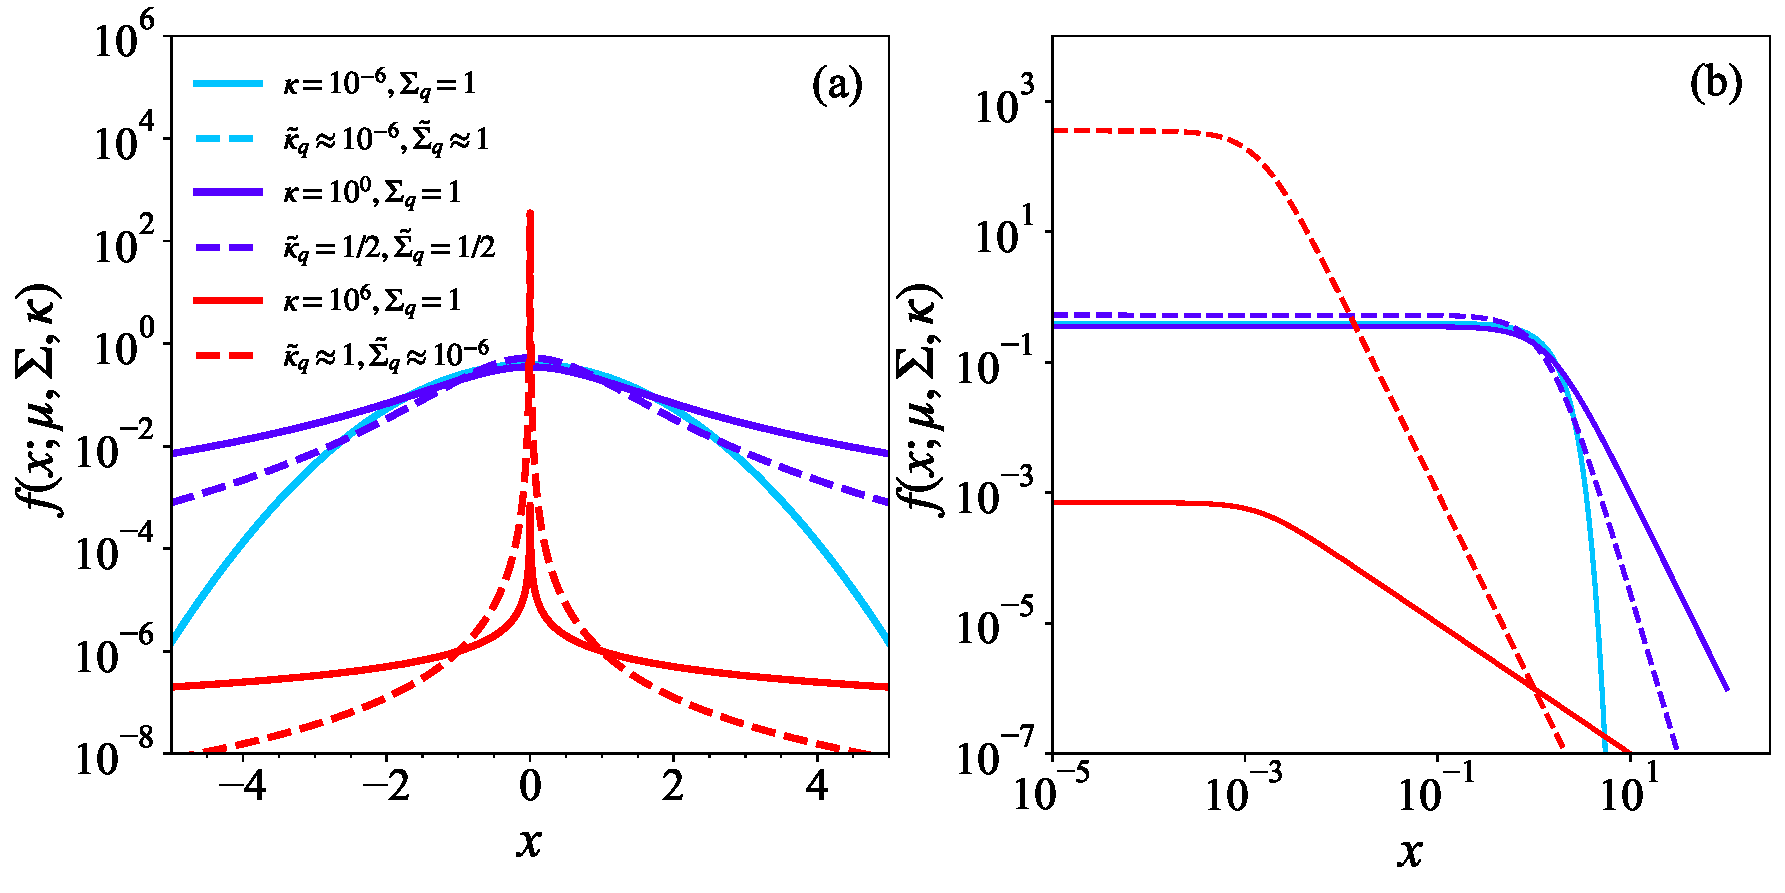
\includegraphics[width=1.0\linewidth]{Fig_Independent_equals_sigma.pdf}
    \caption{\textbf{Independent-equals Distributions.} The plots show coupled Gaussians (solid) and their complementary independent-equals distributions (dashed) for unitary scale $(\Sigma_q=1)$, zero mean ($\mu = 0$) and $\kappa=\{10^{-6}, 10^0, 10^6\}.$ The independent-equals coupled Gaussian has a modified coupling 
    $\tilde{\kappa} = \kappa/(1+\kappa) \approx\{10^{-6},\frac{1}{2}, 1 \}$ 
    and scale $\tilde{\Sigma}_q \approx \Sigma_q/(1+\kappa)=\{1,\frac{1}{2}, \times 10^{-6}\}.$  a) Linear-log axes, and b) log-log axes. For small values of coupling, the modification is negligible, but the deviations become significant for large coupling. The coupled Gaussian approximates a Gaussian for $x\ll \sqrt{2/\kappa}$ and a pure power-law for $x\gg \sqrt{2/\kappa}.$ See Theorem \ref{thm:bending_surface_d_dim} for a proof of the transition point separating Gaussian and power-law behavior.}
    \label{FigIndependentEquals}
\end{figure}

\subsection{The Coupled Free Energy}
With the nonlinear statistical coupling generalization, a spectrum of loss metrics is defined. The coupled log-likelihood is upper bounded by the coupled free energy, which generalizes the free energy, and includes the components of accuracy (cross-entropy) and complexity (divergence).
\begin{equation}
\ln_{\kappa} p(\textbf{x})^\frac{-1}{1+\kappa d/2}\leq
\mathcal{F}_{\theta,\phi,\kappa}(\textbf{x}) = 
\mathbb{E}_{q/^{\iota(\kappa,d_2)}(\textbf{z}\mid \textbf{x})}
\left[\text{ln}_{\kappa}p_\theta(\textbf{x} \mid \textbf{z})^{\frac{-1}{1+\kappa d/2}}\right] + H_{\kappa}\left[q_\phi(\textbf{z}\mid \textbf{x}) \| p_\theta(\textbf{z})\right].
\end{equation}
The generalization uses addition to combine the expected likelihood and the divergence.  The alternative is to use a coupled sum, which introduces a nonlinear interaction between the likelihood and the divergence.  The distinction is whether nonlinear correlation is modeled in the probability domain (regular summation) or in the information domain (coupled sum). The coupled-log likelihood is measured from generated samples based upon draws from the independent-equals posterior distribution, $q/^{\iota(\kappa,d_2)}(\textbf{z}\mid \textbf{x})$, as defined in \ref{equ_IE}. The coupled divergence is also an expectation over the independent-equals posterior distribution. Both of these functions have closed form solutions when the coupling of the metric and distributions match, as shown in the next subsection. 

\begin{figure}[ht!]
    \centering
    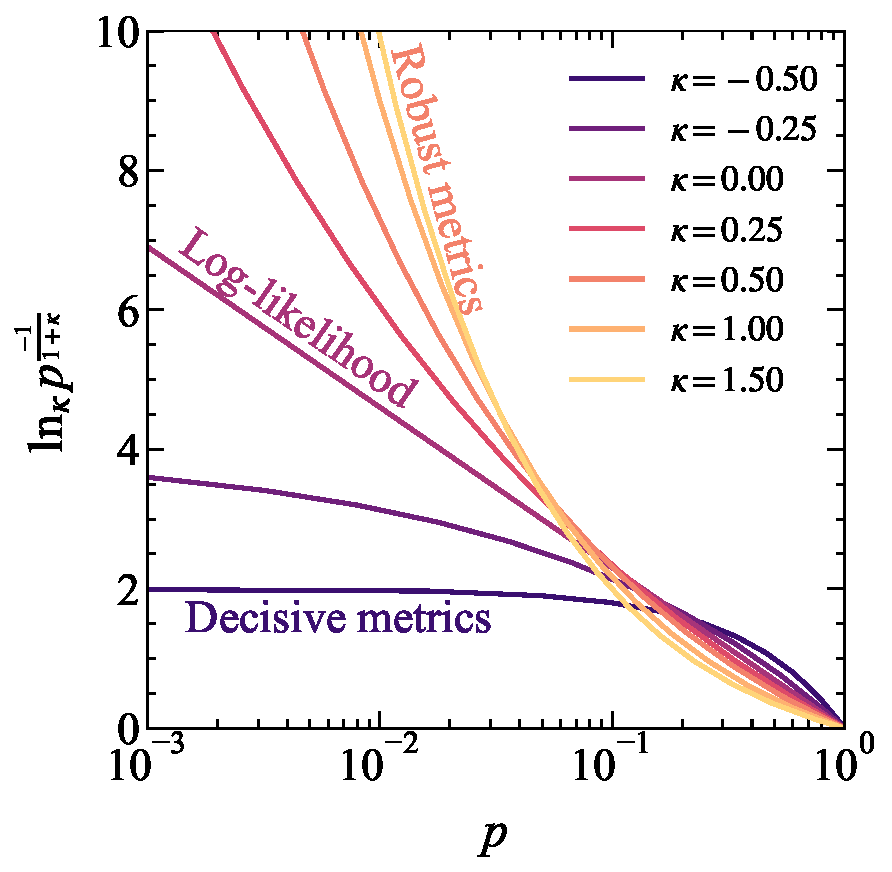
\includegraphics[width=0.6\linewidth]{kappa_log_family.pdf}
    \caption{\textbf{Generalized Coupled logarithm behavior.} In this plot, we show how tuning the nonlinear statistical coupling $\kappa$ dictates the degree of complexity, influencing the tail behavior of distributions. As $\kappa$ increases and $p \rightarrow 0$, the coupled logarithm yields a higher outlier penalty to rare outcomes, increasing the robustness. On the other hand, for $-2/d < \kappa < 0$, the coupled log has decisive behavior, favoring rare probabilities. For $\kappa = 0$, we recover the standard log-likelihood metric.
    }
    \label{kappa_log_family}
\end{figure}

The coupled log-likelihood or coupled cross-entropy is
\begin{align}
&H_\kappa\left(q_\phi(\textbf{z} \mid \textbf{x}),p_\theta(\textbf{x} \mid \textbf{z});2,d\right) \nonumber \\
    &=\mathbb{E}_{q_\phi/^{\iota(\kappa,d_2)}(\textbf{z} \mid \textbf{x})}
    \left[ \ln_{\kappa} p_\theta^{-\frac{1}{1+\kappa d/2}}(\textbf{x} \mid \textbf{z})\right] \nonumber \\
    &=\int_{\mathbf{z}\in \mathcal{X}}
    q_\phi/^{\iota(\kappa,d_22)}(\textbf{z} \mid \textbf{x})
    \ln_{\kappa}p_\theta(\textbf{x} \mid \textbf{z})^{-\frac{1}{1+\kappa d/2}} dq_\phi/^{\iota(\kappa,d_2)}(\textbf{z} \mid \textbf{x}).
\end{align}
The coupled cross-entropy has an important balance in which for positive values of the coupling the coupled logarithm goes to infinity faster for low probability events of $p$; however, this is counter-balanced by the independent-equals distribution $(q/^{\iota(\kappa,d_2)}),$ which has lower scale and shape then the distribution $q$. From this counter-balance, the metric is sensitive to the tail performance while assuring that the training process limits the instability from extreme samples. The coupled divergence is
\begin{align}
&H_\kappa\left(\mathbf{q}||\mathbf{p};2,d\right) \nonumber \\
&=\mathbb{E}_{q_\phi/^{\iota(\kappa,d_2)}
(\textbf{z} \mid \textbf{x})}
\left[ \ln_{\kappa} q_\phi(\textbf{z} \mid \textbf{x})^{-\frac{1}{1+\kappa d/2}}
-\ln_{\kappa} p_\theta(\textbf{z})^{-\frac{1}{1+\kappa d/2}}\right] \nonumber \\
    &=\int_{\mathbf{z}\in \mathcal{X}}
    q_\phi/^{\iota(\kappa,d_2)}
    \left( \ln_{\kappa} q_\phi(\textbf{z} \mid \textbf{x})^{-\frac{1}{1+\kappa d/2}}
    -\ln_{\kappa} p_\theta(\textbf{z})
    ^{-\frac{1}{1+\kappa d/2}}\right)
    dq_\phi/^{\iota(\kappa,d_2)}(\textbf{z} \mid \textbf{x}).
\end{align}
Adding the coupled divergence and coupled cross entropy terms gives the Coupled Free Energy (CFE) used as the optimization objective in the CVAE.

\subsection{Closed form given matching nonlinear nonlinear statistical coupling}

Improved robustness for the VAE can be achieved using a heavy-tailed coupled Gaussian (or Student's t) distribution for the latent and data distributions \citep{caoCoupledVAEImproved2022, kim$t^3$VariationalAutoencoderLearning2023} and/or the coupled free energy metric. In this study we utilize an architecture in which the latent distribution $p_\theta(x)$, data distribution $p_\theta(x|z)$ belong to the coupled Gaussian with a nonlinear statistical coupling $\kappa$ matched to the coupled free energy. This matching condition enables the derivation of a closed form solution for the coupled free energy objective, thereby assuring efficient computation of the gradients. 

The multivariate coupled Gaussian distribution with mean $\boldsymbol{\mu}$ and covariance $\Sigma$ is defined as:
\begin{equation}
\mathcal{N}_{\kappa}(\mathbf{x};\boldsymbol{\mu},\Sigma)
=\frac{1}{Z_{\kappa}(\Sigma, \kappa)}\exp_{\kappa}^{-(1+\kappa d/2)}\!\left(\frac{1}{2}
(\mathbf{x}-\boldsymbol{\mu})^{\top}\Sigma^{-1}(\mathbf{x}-\boldsymbol{\mu})\right),
\end{equation}
where $Z_{\kappa}$ is the normalization constant. Under the matching coupling assumption, the coupled free energy admits closed form expression involving quadratic forms of the type
\[
(\boldsymbol{\mu}_p - \boldsymbol{\mu}_q)^\top
\Sigma_p^{-1}
(\boldsymbol{\mu}_p - \boldsymbol{\mu}_q)
\]
and trace terms such as
\[
\operatorname{tr}(\Sigma_p^{-1}\Sigma_q),
\]
which correspond to Mahalanobis distances and mean-square averages. 

Using the multiplicative property of the coupled exponential, 
\[
\exp_\kappa(x)\exp_\kappa(y)=
\exp_\kappa(x \oplus_\kappa y),
\]
the normalization constant can be absorbed inside the exponential. Specifically,
\[
\frac{1}{Z}\exp_{\kappa}^{-(1+\kappa d/2)}(u)=\exp_{\kappa}^{-(1+\kappa d/2)}
\left(u \oplus_{\kappa} \ln_{\kappa}\left(Z^\frac{1}{1+\kappa d/2}\right)
\right).
\]

Since we are particularly interested in the performance in tails of the distributions, we do not assume that one sample of z and x per input is adequate. 

The coupled free energy with matching coupled Gaussian  distributions simplifies to 
\begin{align}
\mathcal{F}_{\theta,\phi,\kappa}(\mathbf{x})
&= \mathbb{E}_{q_\phi/^{\frac{\kappa}{1+\kappa d/2}}(\mathbf{z}\mid \mathbf{x})}\left[\ln_{\kappa}\left(
p_\theta(\mathbf{x}\mid \mathbf{z})
\right)^{-\frac{1}{1+\kappa d/2}}\right]
\\
&\quad+ \mathbb{E}_{q_\phi/^{\frac{\kappa}{1+\kappa d/2}}(\mathbf{z}\mid\mathbf{x})}
\left[\ln_{\kappa}\left(
q_\phi(\mathbf{z}\mid \mathbf{x})^{-\frac{1}{1+\kappa d/2}}\right) - \ln_{\kappa}
\left(p_\theta(\mathbf{z})^{-\frac{1}{1+\kappa d/2}}\right)\right].
\end{align}

The full derivation and simplified expression are provided in Theorem~\ref{theorem_CFE} (Appendix~B).

The coupled logarithm of a coupled Gaussian, which occurs several times within the coupled ELBO function, simplifies to
\begin{equation}
\ln_{\kappa}\left(\exp_\kappa(y)\right)=y,
\end{equation}
and therefore
\begin{equation}
\ln_{\kappa}
\left[
\left(
\exp_\kappa(y)
\right)^{-(1+\kappa d/2)}
\right]^{-\frac{1}{1+\kappa d/2}}
=
y.
\end{equation}

The simple algebraic form in Theorem~\ref{theorem_CFE} depends on using the same coupling value for both the free energy metric and the probability distributions. Matching these parameters allows the coupled logarithm to undo the exponent of the coupled Gaussian. If instead we evaluate heavy-tailed distributions using the standard free energy metric ($\kappa = 0$), this cancellation does not occur. As shown in Lemma~\ref{lemma:standard_free_energy_coupled_gaussians}, the standard logarithm leaves quadratic terms bound inside logarithmic functions. The resulting integral over the heavy-tailed density cannot be simplified into basic algebra, requiring numerical approximations like Monte Carlo sampling to compute the loss during training.

\section{Experimental Methods}

The experiments evaluate the Coupled Variational Autoencoder (CVAE) across standard image datasets (CelebA and MNIST) and extreme financial data (cryptocurrency daily log-returns). The primary purpose is to build a generative model capable of learning in extreme environments where the data exhibits heavy tails and diverging first or second moments. To build a robust model, the CVAE uses the Coupled Free Energy loss function, which enables the neural network's decoder to act as a nonlinear amplifier, processing compact, stable latent vectors and projecting them into extreme, heavy-tailed data outputs.

It is important to consider that heavy-tailed distributions are non-ergodic, meaning that a single random sample rarely reflects the system's true average behavior. To account for this, the numerical computation of the Coupled Free Energy requires an ensemble approach. For each input, the model generates a summation of $S$ different samples. The loss is then averaged across these samples and the batch before updating the network weights using standard backpropagation. Future research may improve training efficiency by using the natural gradients of the coupled exponential family.

In algorithm \ref{alg:cvae_training} we detail the core logic of the model. During Phase 1, the model trains using the independent-equals expectation. This reduces the variance of the latent space, keeping the neural network numbers small and stable to prevent numerical collapse. During Phase 2, this safety scaling is removed. It is crucial to drop the scaling during inference because physical reality, such as extreme financial volatility, follows the original heavy-tailed distribution. By drawing samples directly from the unscaled distribution, we force the model to prove it can genuinely generate the extreme data events it learned to map during training.

\begin{algorithm}[H]
\caption{Coupled Variational Autoencoder (CVAE): Training and Inference}
\label{alg:cvae_training}
\begin{algorithmic}[1]
\Require Full Dataset $\mathcal{D}$ partitioned into $\mathcal{D}_{train}$, $\mathcal{D}_{val}$, and $\mathcal{D}_{test}$
\Require Target Coupling $\kappa$, Latent Dimension $d$, Batch Size $B$, Samples $S$, Epochs $E$
\Require Adam Optimizer with Learning Rate $\eta$
\State Initialize Encoder weights $\phi$ and Decoder weights $\theta$
\Statex
\State \textbf{Phase 1: Training (using Independent-Equals expectation)}
\For{$epoch = 1, \dots, E$}
    \For{mini-batch $X$ of size $B$ in $\mathcal{D}_{train}$}
        \State $\mu_q, \log\sigma_q^2 \leftarrow \text{Encoder}_\phi(X)$
        \State $\sigma_q \leftarrow \exp(0.5 \cdot \log\sigma_q^2)$
        \Statex
        \State \Comment{Apply Independent-Equals (IE) Scaling to safeguard gradients (Lemma 2)}
        \State $\tilde{\kappa} \leftarrow \frac{\kappa}{1+\kappa}$
        \State $\tilde{\sigma}_q \leftarrow \frac{\sigma_q}{\sqrt{1+\kappa}}$
        \Statex
        \State Initialize batch loss $\mathcal{F}_{batch} \leftarrow 0$
        \State \Comment{Draw $S$ samples per input to overcome nonergodicity}
        \For{$s = 1, \dots, S$}
            \State \Comment{Sample $d$-dimensional noise using scaled parameters}
            \State Draw $\epsilon_s \sim \text{MCG}(\tilde{\kappa}, I_d)$ 
            \State $Z_s \leftarrow \mu_q + \tilde{\sigma}_q \odot \epsilon_s$
            \State $\hat{X}_s \leftarrow \text{Decoder}_\theta(Z_s)$
            \Statex
            \State \Comment{Accumulate the Coupled Free Energy}
            \State $\mathcal{F}_{batch} \leftarrow \mathcal{F}_{batch} + \frac{1}{S} \mathcal{F}_{\theta, \phi, \kappa}(X, \hat{X}_s, Z_s)$
        \EndFor
        \Statex
        \State \Comment{Backpropagate the averaged ensemble loss}
        \State Update $\theta, \phi$ by descending $\nabla_{\theta, \phi} \mathcal{F}_{batch}$ using Adam($\eta$)
    \EndFor
\EndFor
\Statex
\State \textbf{Phase 2: Inference / Reconstruction (using Original Heavy-Tailed Distribution)}
\For{mini-batch $X_{test}$ in $\mathcal{D}_{test}$}
    \State $\mu_q, \log\sigma_q^2 \leftarrow \text{Encoder}_\phi(X_{test})$
    \State $\sigma_q \leftarrow \exp(0.5 \cdot \log\sigma_q^2)$
    \Statex
    \State \Comment{Sample using Original Distribution (No Independent-Equals Scaling)}
    \State \Comment{Draw 1 $d$-dimensional sample to test true generative variance}
    \State Draw noise $\epsilon \sim \text{MCG}(\kappa, I_d)$
    \State $Z_{test} \leftarrow \mu_q + \sigma_q \odot \epsilon$
    \State $\hat{X}_{test} \leftarrow \text{Decoder}_\theta(Z_{test})$
    \State \Return $\hat{X}_{test}$ for evaluation metrics.
\EndFor
\end{algorithmic}
\end{algorithm}

Algorithm \ref{alg:cvae_robustness} describes the process for testing model robustness. Physical corruptions, such as fog or blur, are applied to the input data. The encoder maps this degraded image into the heavy-tailed latent space. The wide tails of this distribution absorb the extreme variations caused by the noise, allowing the decoder to focus on the underlying structure. The resulting image is evaluated against the clean original data to verify structural recovery.

\begin{algorithm}[H]
\caption{CVAE Robustness Inference (Image Corruptions)}
\label{alg:cvae_robustness}
\begin{algorithmic}[1]
\Require Clean Test Dataset $\mathcal{D}_{test}$
\Require Pre-trained $\text{Encoder}_\phi$ and $\text{Decoder}_\theta$
\Require Target Coupling $\kappa$, Latent Dimension $d$
\Require Set of Corruption Functions $\mathcal{C} = \{\text{Gaussian Noise, Motion Blur, Fog, Shot Noise}\}$
\Statex
\For{each corruption function $C \in \mathcal{C}$}
    \State Initialize metric accumulators for $C$ (e.g., FID, SSIM)
    \For{mini-batch $X_{clean}$ in $\mathcal{D}_{test}$}
        \State \Comment{Apply physical corruption to the input}
        \State $X_{corr} \leftarrow C(X_{clean})$
        \Statex
        \State \Comment{Encode the degraded image}
        \State $\mu_q, \log\sigma_q^2 \leftarrow \text{Encoder}_\phi(X_{corr})$
        \State $\sigma_q \leftarrow \exp(0.5 \cdot \log\sigma_q^2)$
        \Statex
        \State \Comment{Sample using Original Heavy-Tailed Distribution (No IE Scaling)}
        \State \Comment{The heavy tail acts as a shock absorber for the noise}
        \State Draw $d$-dimensional noise $\epsilon \sim \text{MCG}(\kappa, I_d)$
        \State $Z_{corr} \leftarrow \mu_q + \sigma_q \odot \epsilon$
        \Statex
        \State \Comment{Decode back to image space}
        \State $\hat{X}_{recon} \leftarrow \text{Decoder}_\theta(Z_{corr})$
        \Statex
        \State \Comment{Evaluate structural recovery against the CLEAN original, not the corrupted input}
        \State Compute metrics comparing $\hat{X}_{recon}$ to $X_{clean}$
        \State Accumulate metrics
    \EndFor
    \State \Return Final aggregated robustness scores for corruption $C$
\EndFor
\end{algorithmic}
\end{algorithm}

Algorithm \ref{alg:cvae_stochastic} details the deep tail exploration process. A single test image is encoded, and the model generates $N$ decoded samples from that specific latent coordinate. We compute the squared Euclidean distance ($|| \hat{x}_i - x_{test} ||_2^2$) between each generated image and the original image to rank the reconstructions from best to worst. Using the squared distance avoids computationally expensive square root operations while preserving the correct order. This experiment reveals the true boundaries of the learned latent space, demonstrating what happens when the network encounters the rare, massive numbers drawn from the deep tails of the distribution. By analyzing the worst reconstructions, we can observe how the model interprets extreme uncertainty and verify that the decoder handles massive inputs without numerical failure.

\begin{algorithm}[H]
\caption{CVAE Stochastic Consistency Analysis (Deep Tail Exploration)}
\label{alg:cvae_stochastic}
\begin{algorithmic}[1]
\Require Single Unseen Test Image $x_{test} \in \mathcal{D}_{test}$
\Require Pre-trained $\text{Encoder}_\phi$ and $\text{Decoder}_\theta$
\Require Target Coupling $\kappa$, Latent Dimension $d$
\Require Total Samples $N$, Compute Batch Size $B$
\Statex
\State \Comment{Encode the single image once to establish the latent cluster center}
\State $\mu_q, \log\sigma_q^2 \leftarrow \text{Encoder}_\phi(x_{test})$
\State $\sigma_q \leftarrow \exp(0.5 \cdot \log\sigma_q^2)$
\Statex
\State Initialize empty list $\mathcal{R}$ to store squared Euclidean distances
\State Initialize empty list $\mathcal{Z}_{all}$ to store all generated latent vectors
\Statex
\State \Comment{Process in batches to prevent memory overflow}
\For{$iteration = 1 \dots \frac{N}{B}$}
    \State \Comment{Draw $B$ independent $d$-dimensional samples using Original Distribution}
    \State Draw noise batch $\epsilon \sim \text{MCG}(\kappa, I_d)$ of size $B$
    \State $Z_{batch} \leftarrow \mu_q + \sigma_q \odot \epsilon$
    \State Store $Z_{batch}$ in $\mathcal{Z}_{all}$
    \Statex
    \State \Comment{Decode the batch of samples}
    \State $\hat{X}_{batch} \leftarrow \text{Decoder}_\theta(Z_{batch})$
    \Statex
    \State \Comment{Calculate squared Euclidean distance from the original image for each sample}
    \For{each $\hat{x}_i$ in $\hat{X}_{batch}$}
        \State $r_i \leftarrow || \hat{x}_i - x_{test} ||_2^2$ 
        \State Append $r_i$ to $\mathcal{R}$
    \EndFor
\EndFor
\Statex
\State \Comment{Sort distances to map the extremes of the physical data manifold}
\State $Indices_{sorted} \leftarrow \text{Argsort}(\mathcal{R})$
\State Extract indices for the 16 smallest, 32 median, and 16 largest distances
\Statex
\State \Comment{Generate visualizations}
\State $Z_{selected} \leftarrow \text{Extract}(\mathcal{Z}_{all}, Indices_{selected})$
\State $\hat{X}_{grid} \leftarrow \text{Decoder}_\theta(Z_{selected})$
\State Save $\hat{X}_{grid}$ as an $8 \times 8$ structured grid
\State Compute and save normalized histogram of $\mathcal{R}$
\end{algorithmic}
\end{algorithm}

\subsection{Architecture}
\textcolor{red}{update}
To empirically evaluate the coupled variational autoencoder, or CVAE, we trained dense neural networks on X of the MNIST hand-written digit data set and convolutional neural networks on Y of the CIFAR image data set and tested them on the hold-out images, along with corrupted versions of those images. The corruptions tested were [list of corruptions]. We varied the $\kappa_{loss}$ from 0, which is the standard loss function, and [list values]. We evaluated the generalized means of the test set losses at -2/3, 0, and 1. [Discuss what each metric tells us about the network performance]. Random seeds were set according to the [microseconds?] up to the runtime point. The networks were trained until [Z] successive epochs without reduction in the evaluation set coupled loss.
The dense neural network architectures were [discuss layers, parameters, make an image displaying it]. The convolutional architectures were [discuss layers, parameters, make an image displaying it]. [Why did we choose those architectures?] The deep learning framework used to implement them is tensorflow.




       
\section{Results} 

In this section, we show the initial results of the CVAE performance. To train the model, we consider the CelebA dataset (CelebFaces Attributes Dataset), a widely used dataset for computer vision tasks involving human faces. This data set contains $202,599$ images of celebrity faces with high variability and visual richness, making it an ideal benchmark for learning complex data distributions and testing the performance of generative models. For testing purposes, we use an image size of $128\times128$ (original images are $178\times178$), a batch size of $64$ images, a learning rate of $ 5\times10^ {-4}$, and a latent dimension of $d =100$.

\begin{figure}[ht!]
        \centering
		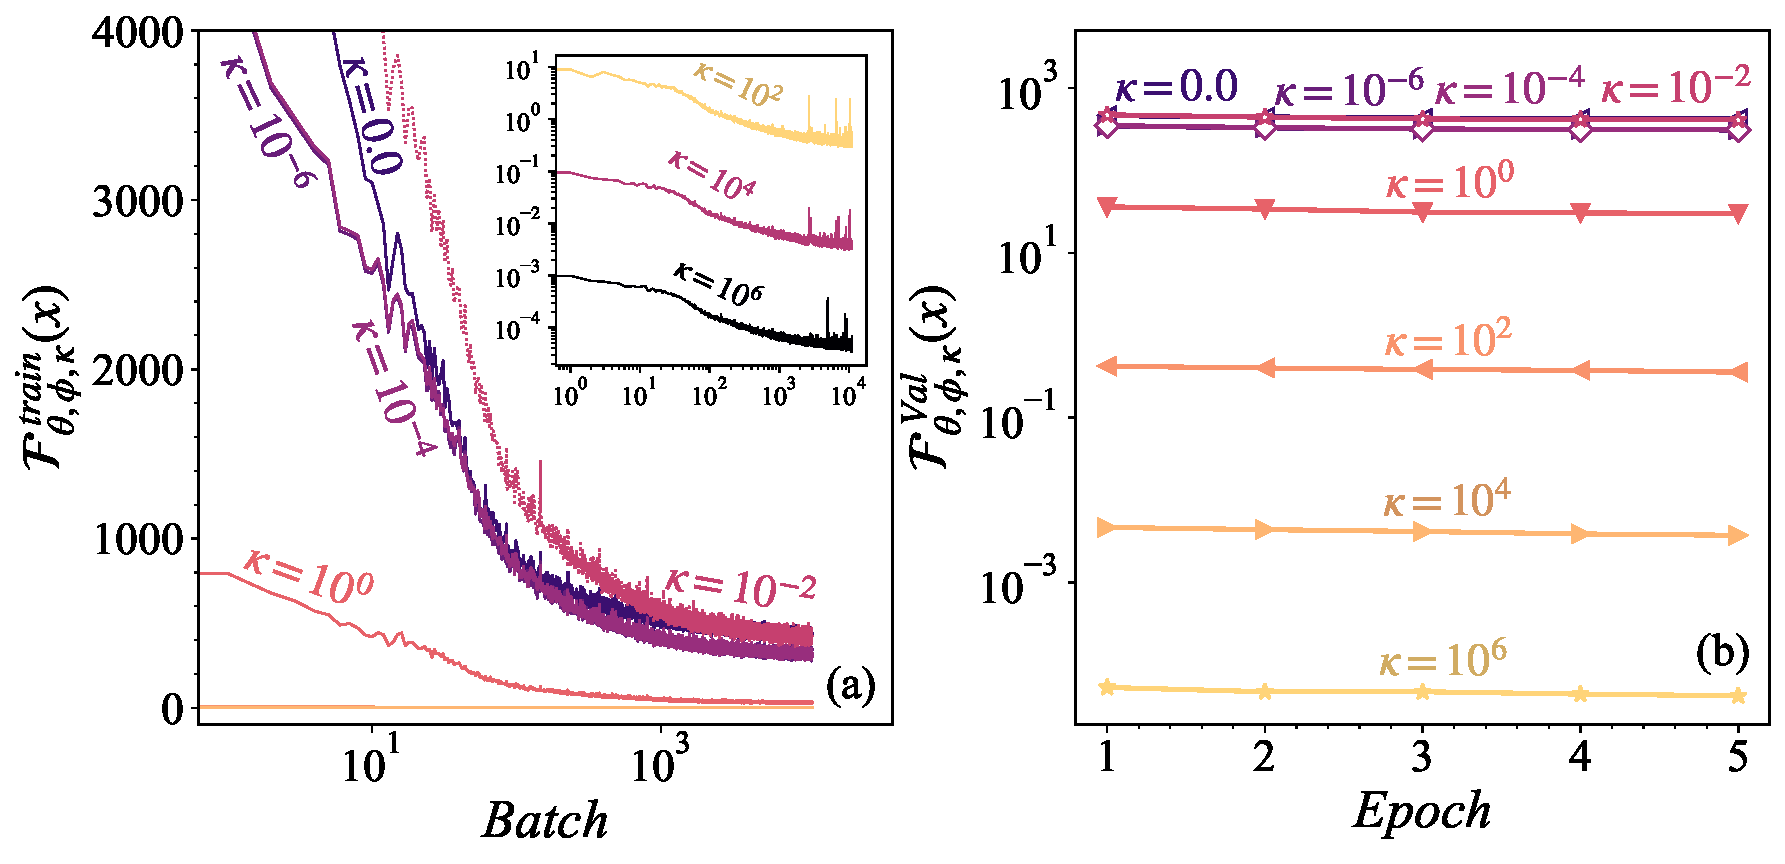
\includegraphics[width= \linewidth]{Fig_Energy.pdf} 
            \caption{Comparison of the Coupled Free Energy across different values of the coupling parameter $\kappa$ for both (A) training and (B) validation phases using diagonal covariance. The models are trained and validated using the Independent equals distribution. The inset in panel (A) shows the train Coupled Free Energy of the most extreme models over the batches on a log-log scale.}
		\label{Fig_energy.png}
\end{figure}

The model was trained using Adam Optimizer and without a learning rate scheduler. To ensure reproducibility and consistent weight initialization, all linear and transposed convolution layers were initialized using the Kaiming uniform method (for layers with LeakyReLU activations), while linear layers used Xavier initialization. Batch normalization layers were initialized with unit scale and zero bias, and their running statistics were reset when loading checkpoints, helping stabilize the internal covariate shift during training. The CelebA data set was randomly split into $70\%$ training, $15\% $ validation, and $15\%$ test sets, and the data was shuffled at the beginning of each epoch. The models were trained and validated using samples from the independent equals distribution. For validation and testing, samples were drawn from the coupled Gaussian and the independent equals distribution for comparison. A fixed batch of validation images generated consistent reconstructions and samples across epochs for visual assessment.

The architecture employed for the VAE and CVAE models consists of a convolutional encoder-decoder structure. The encoder is built from four convolutional layers with increasing depth (32 to 256 channels), followed by batch normalization and LeakyReLU activation functions. The encoded feature map is flattened and passed through two linear layers to produce the latent mean and log-variance vectors. The decoder mirrors the encoder structure with transposed convolutions, batch normalization, and LeakyReLU activations, culminating in a final Sigmoid layer to map outputs to the $[0, 1]$ range. 

We conducted the experiments using PyTorch's automatic differentiation framework (autograd), which computes gradients based on the standard Euclidean geometry of the parameter space. Although this approach is sufficient for baseline comparisons and initial performance assessments, it does not account for the curved geometry induced by the coupled exponential family. Future work will incorporate the information geometric formulation introduced in this paper, using the analytically derived gradients and curvature-aware optimization based on the coupled free energy. This is expected to improve the efficiency and stability of the learning convergence by aligning the optimization trajectory with the intrinsic geometry of the coupled statistical manifold.

In Fig. \ref{Fig_energy.png} we show that the CVAE with $\kappa = 10^{-5}$ produces a stationary energy similar to the standard VAE $(\kappa=0)$, but the CVAE with $\kappa = 1, 10$ and $\kappa = 10^5$ shows significantly lower coupled free energy with both the training and validation data. Additionally, the CVAE energy curves with positive coupling are less noisy and have fewer and smaller spikes, which may indicate that the coupled model was trained more robustly. Because the coupled free energy metric varies with the coupling, these measurements do not provide a direct comparison; however, as the coupling increases, the metric increases in sensitivity and can rise above the $\kappa=0$ metric if the algorithm lacks robustness. For comparison, Fig. \ref{Fig_reconstructions.png} shows the standard and coupled VAE reconstructions, with the latter capturing higher fidelity.
\begin{figure}[ht!]
	   \centering
		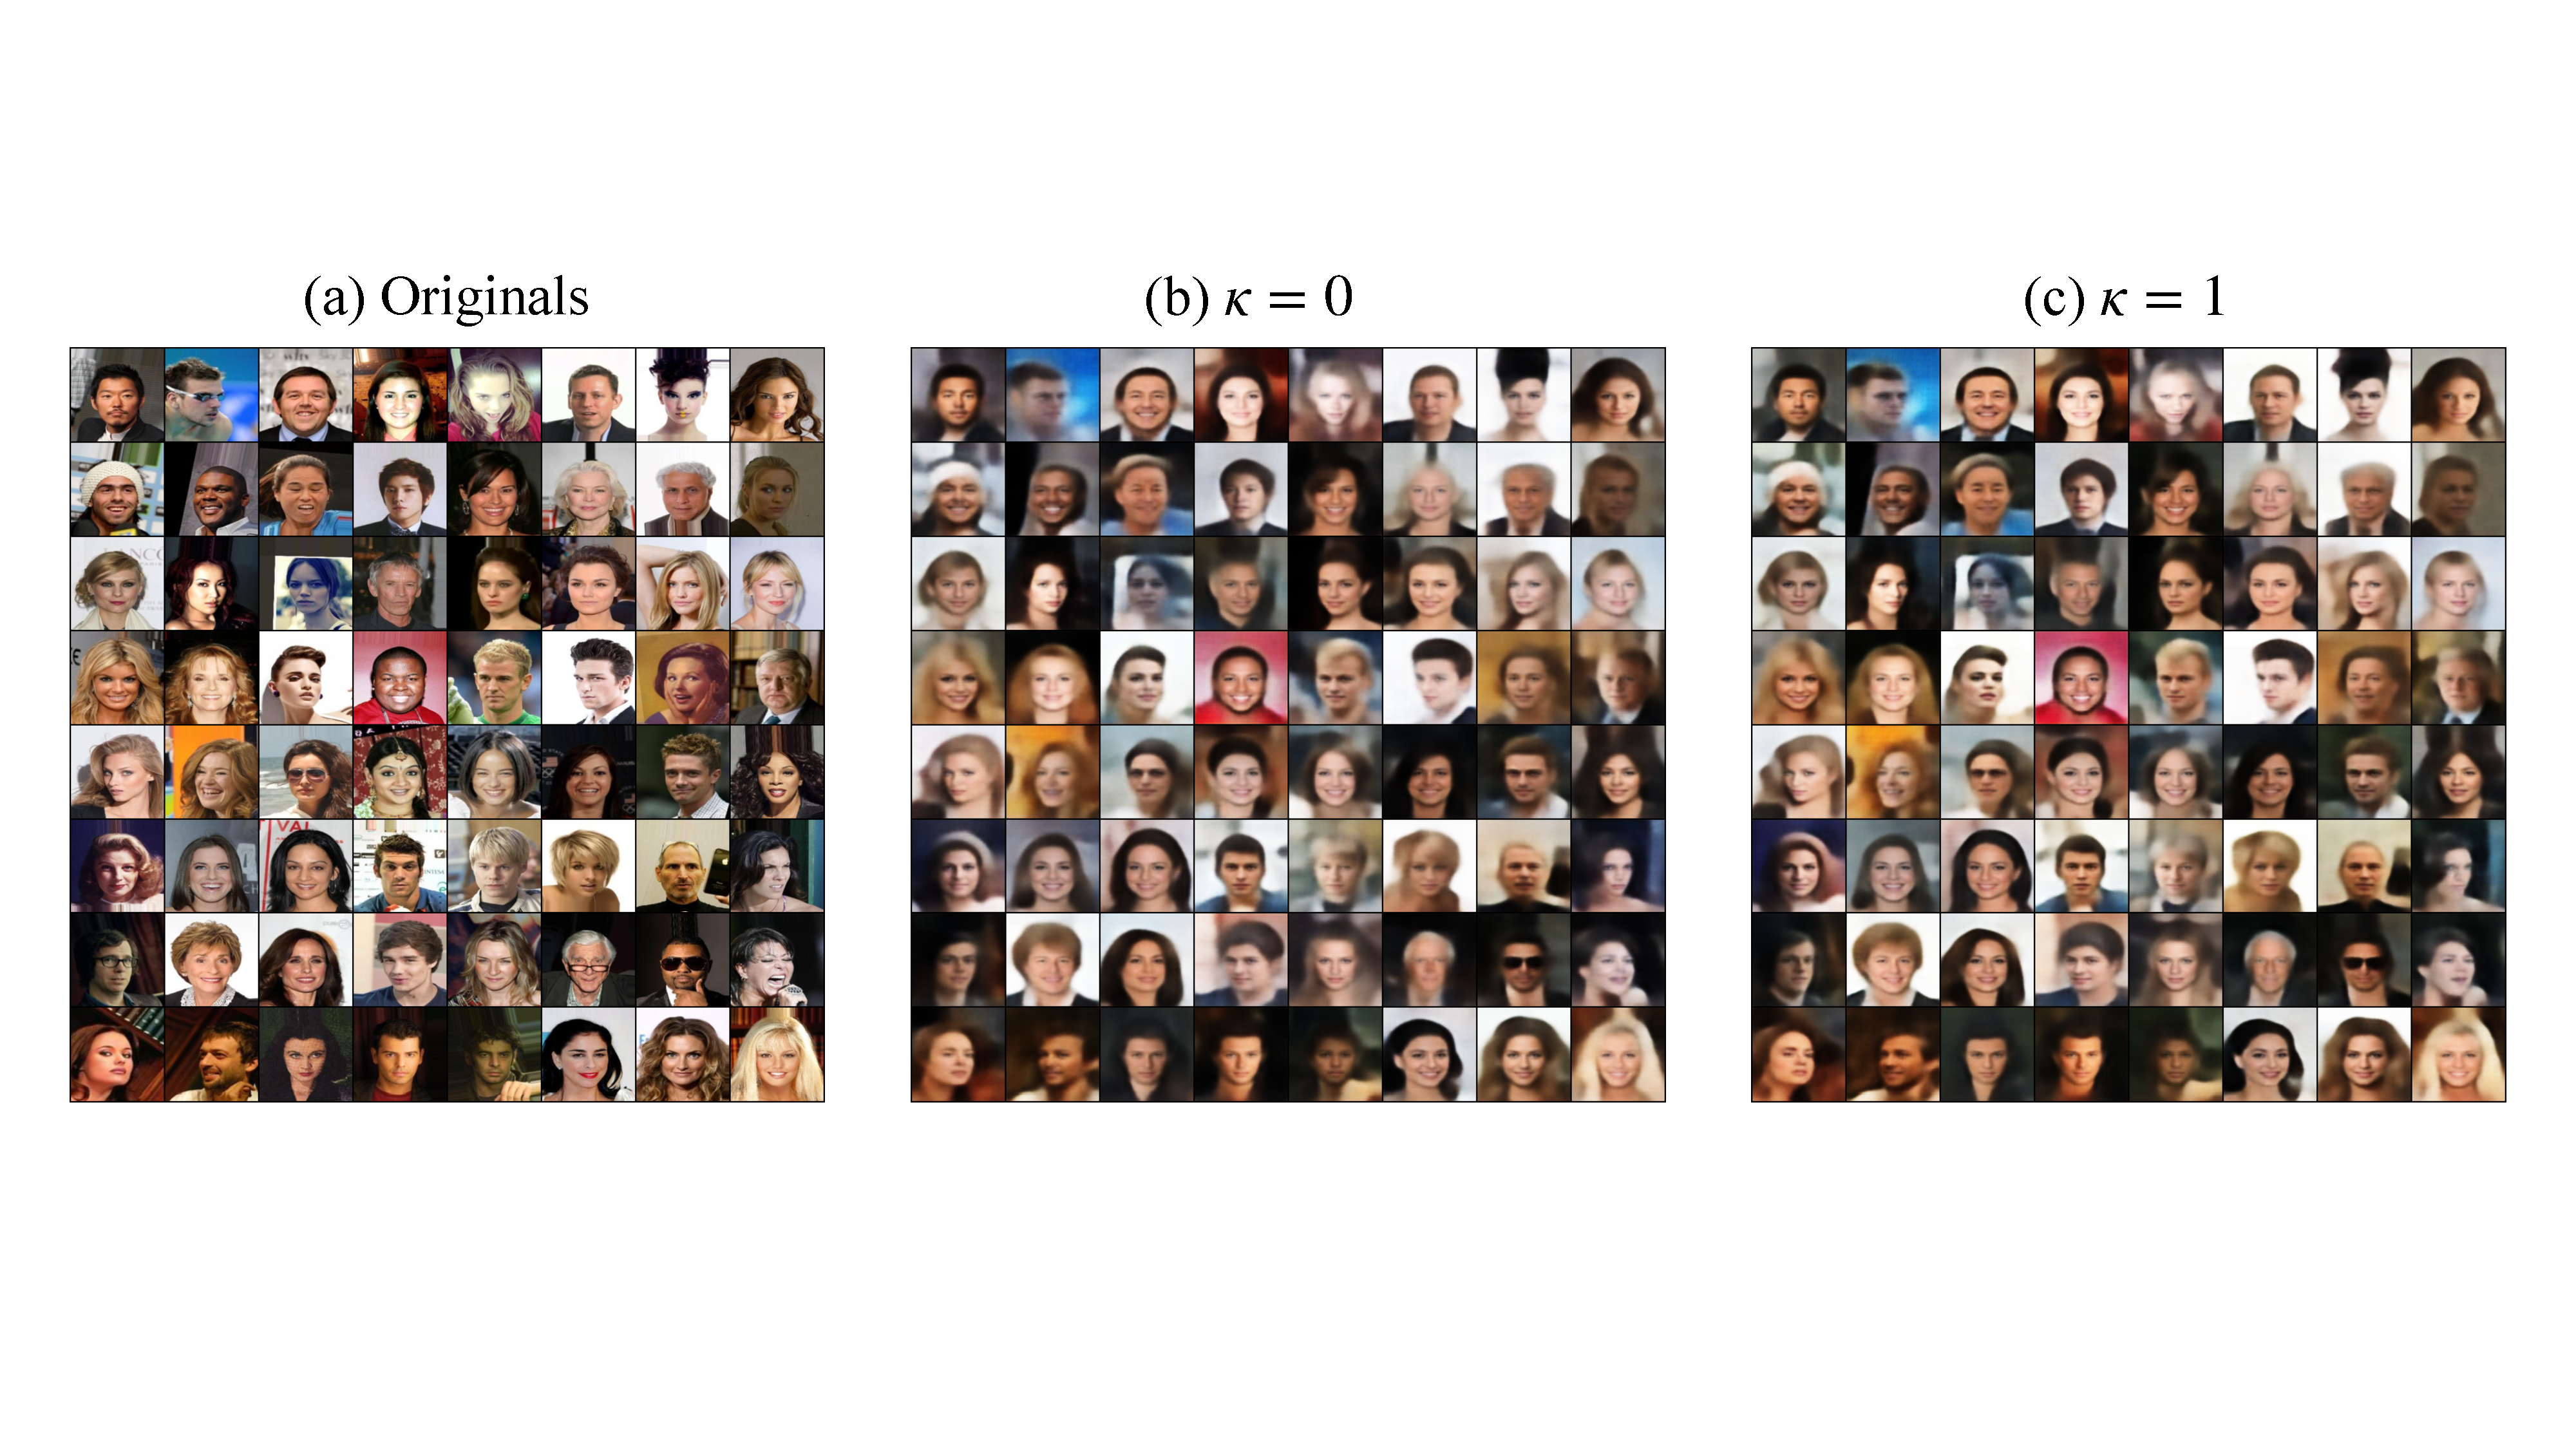
\includegraphics[width= \linewidth]{recons.pdf} 
           \caption{Comparison of the standard linear correlation and the long-range coupling models.  (a) Original images and reconstructions with (b) Diagonal standard VAE and (c) Diagonal Coupled VAE with $\kappa = 1$. }
		\label{Fig_reconstructions.png}
\end{figure}

\begin{figure}[ht!]
	   \centering
		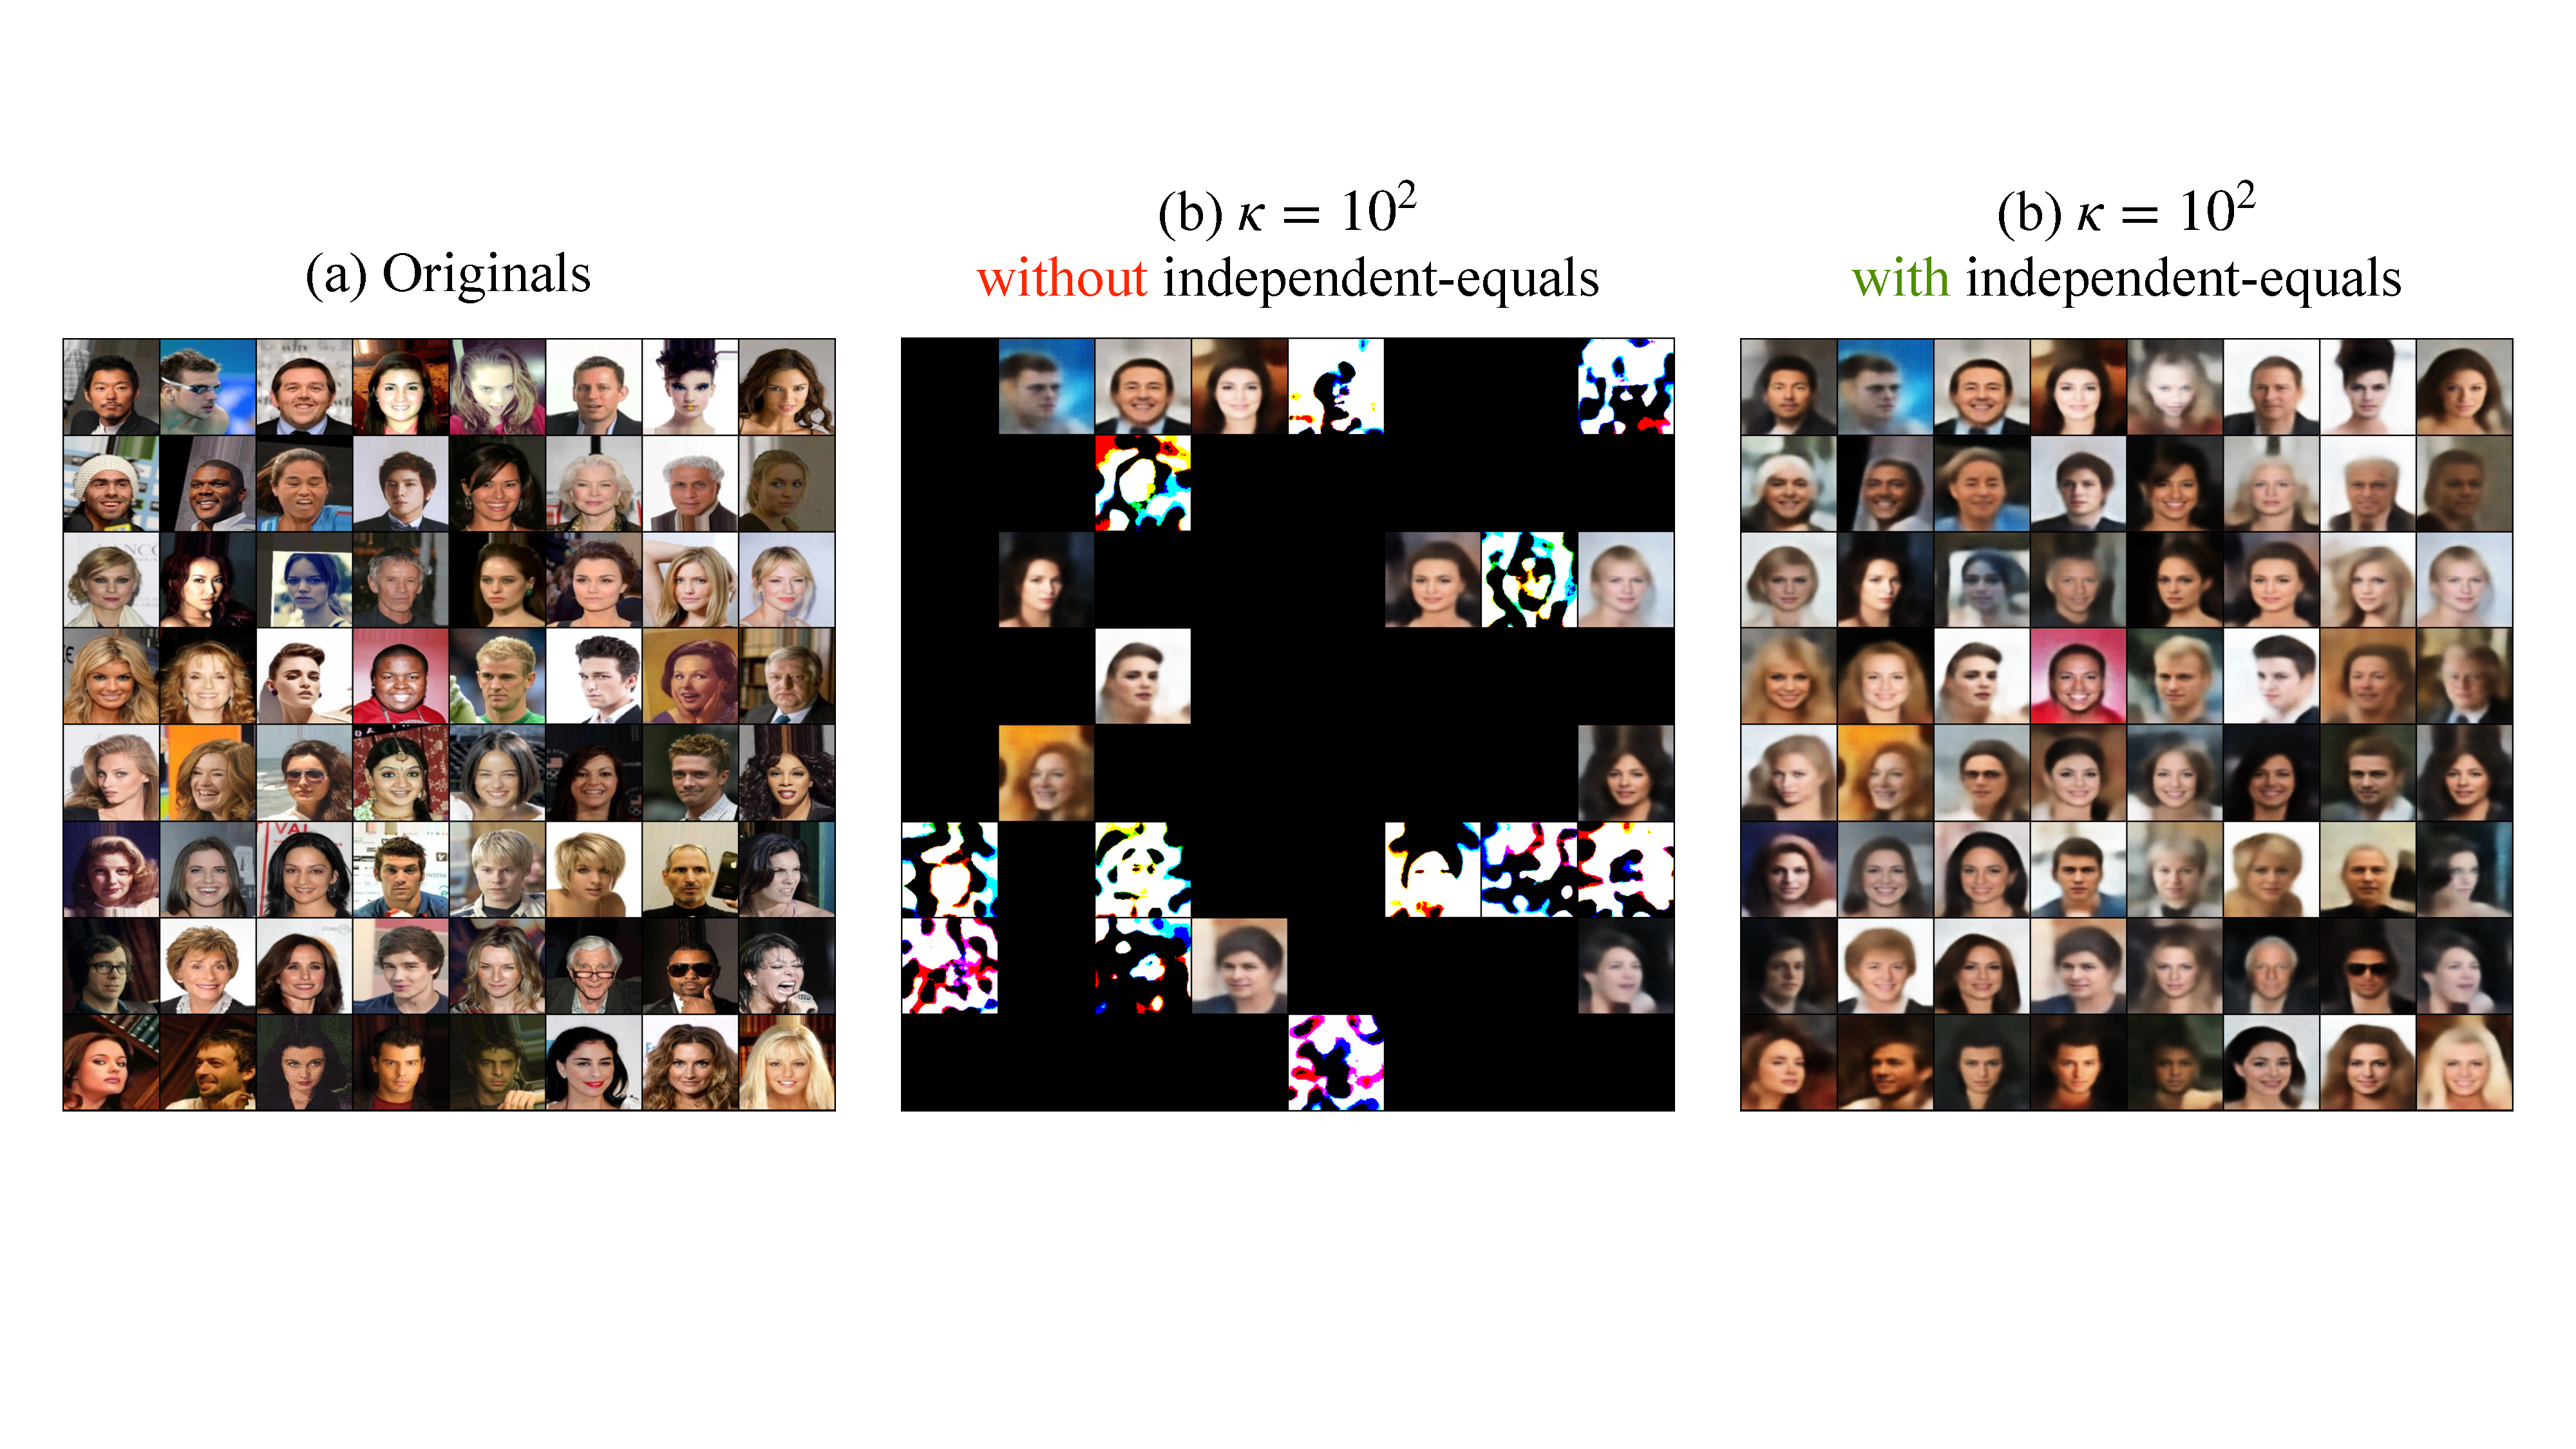
\includegraphics[width= \linewidth]{extremeComp.pdf} 
           \caption{Comparison between the (a) Original images and generated reconstructions of the coupled CVAE with extreme coupling $\kappa = 10^2$ (b) without and (c) with using the independent-equals sampling. We emphasize, however, that both models were trained using the Independent-equals distribution. Training for nonlinearities as $\kappa = 10^2$ without using the independent-equals generates NANs that invalidate the training process.}
		\label{fig:extreme_coupling_recons}
\end{figure}

We employ several widely used metrics to assess the quality of the generated reconstructions. These include the Fréchet Inception Distance (FID), which quantifies the similarity between the feature distributions of original and reconstructed images via an Inception-v3 network. The Kernel Inception Distance (KID) is a related metric based on a polynomial kernel and the maximum mean discrepancy. The Learned Perceptual Image Patch Similarity (LPIPS) assesses perceptual similarity by comparing deep network features extracted from a pre-trained AlexNet. We also use Peak Signal-to-Noise Ratio (PSNR) for pixel-level reconstruction accuracy, and the Structural Similarity Index Measure (SSIM) for analyzing structural information and perceived image quality. The Fréchet ResNet Distance (FRD) leverages features from a ResNet-50 backbone. Finally, Precision and Recall evaluate the fidelity and coverage of the reconstructed image distribution. We calculated Precision and Recall using a K-Nearest Neighbors manifold algorithm with 20 neighbors to ensure a robust evaluation of the boundaries in high-dimensional space.

We evaluate the generative performance of the Coupled VAE against the standard VAE baseline ($\kappa=0$). Table \ref{tab:metrics_absolute} presents the absolute scores across all metrics. The baseline model assumes the data fits an exponential distribution, which fails when modeling extreme outliers of the dataset. The data confirm that the generative quality improves with $\kappa > 0$, where the model is a heavy-tailed distribution, reaching peak performance at $\kappa = 10^0 = 1$. Due to the independent-equals sampling, the neural network weights remain stable even at extreme nonlinearities such as $\kappa \ge 10^2$. Even as performance degrades toward extreme nonlinearity, the model still generates meaningful reconstructions and beats the baseline VAE. 

Table \ref{tab:metrics_improvement} illustrates the relative percentage improvements over the baseline. Capturing the heavy tails yields measurable gains across all criteria. At the optimal $\kappa = 10^0 = 1$ setting, the model achieves a 10\% improvement in perceptual similarity (LPIPS) and a 13\% gain in feature distribution matching (FRD). Expanding the manifold search to 20 neighbors reveals that generative coverage improves dramatically as well. By utilizing the independent-equals expectation during sampling, the coupled models achieve up to an 8\% increase in Precision and a 70\% increase in Recall compared to the baseline.

\begin{table}[h!]
\centering
\renewcommand{\arraystretch}{1.4}
\setlength{\tabcolsep}{6pt}
\small
\begin{tabular}{lcccccccc}
\toprule
\rowcolor{gray!20}
\textbf{$\kappa$} & \textbf{FID} & \textbf{KID} & \textbf{LPIPS} & \textbf{SSIM} & \textbf{PSNR} & \textbf{FRD} & \textbf{Prec} & \textbf{Rec} \\
\midrule
$0.0$        & 113.7 & 0.115(7) & 0.37(2) & 0.59(2) & 20.3(6) & 295 & 0.755 & 0.023 \\
$10^{-6}$    & \textcolor{blue}{109.2} & \textcolor{blue}{0.111(6)} & \textcolor{blue}{0.35(2)} & \textcolor{blue}{0.62(2)} & \textcolor{blue}{21.0(7)} & \textcolor{blue}{266} & \textbf{\textcolor{green!50!black}{0.816}} & \textcolor{blue}{0.035} \\
$10^{-4}$    & \textcolor{blue}{106.2} & \textcolor{blue}{0.108(6)} & \textcolor{blue}{0.35(2)} & \textcolor{blue}{0.62(2)} & \textcolor{blue}{21.0(7)} & \textcolor{blue}{259} & \textcolor{blue}{0.800} & \textcolor{blue}{0.035} \\
$10^{-2}$    & \textcolor{blue}{106.1} & \textcolor{blue}{0.108(6)} & \textcolor{blue}{0.34(2)} & \textcolor{blue}{0.62(2)} & \textcolor{blue}{21.1(7)} & \textcolor{blue}{261} & \textcolor{blue}{0.813} & \textbf{\textcolor{green!50!black}{0.039}} \\
$10^{0}$     & \textbf{\textcolor{green!50!black}{104.0}} & \textbf{\textcolor{green!50!black}{0.106(5)}} & \textbf{\textcolor{green!50!black}{0.33(2)}} & \textbf{\textcolor{green!50!black}{0.63(2)}} & \textbf{\textcolor{green!50!black}{21.5(7)}} & \textbf{\textcolor{green!50!black}{258}} & \textcolor{blue}{0.815} & \textcolor{blue}{0.035} \\
$10^{2}$     & \textcolor{blue}{110.3} & \textcolor{blue}{0.112(6)} & \textcolor{blue}{0.34(2)} & \textcolor{blue}{0.62(2)} & \textcolor{blue}{21.3(7)} & \textcolor{blue}{262} & \textbf{\textcolor{green!50!black}{0.816}} & \textcolor{blue}{0.027} \\
$10^{4}$     & \textcolor{blue}{108.9} & \textcolor{blue}{0.112(7)} & \textcolor{blue}{0.34(2)} & \textcolor{blue}{0.63(2)} & \textcolor{blue}{21.4(7)} & \textcolor{blue}{263} & \textcolor{blue}{0.814} & \textcolor{blue}{0.034} \\
$10^{6}$     & \textcolor{blue}{110.1} & \textcolor{blue}{0.112(7)} & \textcolor{blue}{0.35(2)} & \textcolor{blue}{0.62(2)} & \textcolor{blue}{21.4(7)} & \textcolor{blue}{264} & \textcolor{blue}{0.805} & \textcolor{blue}{0.032} \\
\bottomrule
\end{tabular}
\caption{Comprehensive evaluation of reconstruction quality across different values of $\kappa$ in the Coupled Variational Autoencoder (CVAE). Metrics include Fréchet Inception Distance (FID), Kernel Inception Distance (KID), LPIPS, SSIM, PSNR, Fréchet ResNet Distance (FRD), Precision, and Recall. The standard Gaussian baseline corresponds to $\kappa = 0$. Values highlighted in \textcolor{blue}{blue} indicate performance superior to the baseline, while the best overall result for each metric is highlighted in \textbf{\textcolor{green!50!black}{bold green}}. Note that FID, FRD, Precision, and Recall are presented without standard deviations, as these geometric and distributional metrics are computed holistically across the entire dataset manifold rather than averaged across batches. To ensure statistical rigor, each model generated exactly 10,000 reconstructions evaluated 1-to-1 against an identical ground-truth subset. The results demonstrate that all coupled configurations outperform the standard uncoupled baseline and remain highly stable even at extreme nonlinearities ($\kappa \ge 10^2$). The coupling $\kappa = 10^{0} = 1$ yields the overall optimal trade-off. The value in parentheses denotes the measured standard deviation spread formatted to one significant digit.} 
\label{tab:metrics_absolute}
\end{table}

\begin{table}[h!]
\centering
\renewcommand{\arraystretch}{1.4}
\setlength{\tabcolsep}{6pt}
\small
\begin{tabular}{lcccccccc}
\toprule
\rowcolor{gray!20}
\textbf{$\kappa$} & \textbf{FID} & \textbf{KID} & \textbf{LPIPS} & \textbf{SSIM} & \textbf{PSNR} & \textbf{FRD} & \textbf{Prec} & \textbf{Rec} \\
\midrule
$10^{-6}$    & \textcolor{blue}{4\%} & \textcolor{blue}{3(7)\%} & \textcolor{blue}{7(6)\%} & \textcolor{blue}{4(4)\%} & \textcolor{blue}{4(5)\%} & \textcolor{blue}{10\%} & \textbf{\textcolor{green!50!black}{8\%}} & \textcolor{blue}{52\%} \\
$10^{-4}$    & \textcolor{blue}{7\%} & \textcolor{blue}{6(7)\%} & \textcolor{blue}{7(6)\%} & \textcolor{blue}{4(4)\%} & \textcolor{blue}{4(5)\%} & \textcolor{blue}{12\%} & \textcolor{blue}{6\%} & \textcolor{blue}{52\%} \\
$10^{-2}$    & \textcolor{blue}{7\%} & \textcolor{blue}{6(7)\%} & \textcolor{blue}{8(6)\%} & \textcolor{blue}{4(4)\%} & \textcolor{blue}{4(5)\%} & \textcolor{blue}{12\%} & \textcolor{blue}{8\%} & \textbf{\textcolor{green!50!black}{70\%}} \\
$10^{0}$     & \textbf{\textcolor{green!50!black}{9\%}} & \textbf{\textcolor{green!50!black}{8(7)\%}} & \textbf{\textcolor{green!50!black}{10(6)\%}} & \textbf{\textcolor{green!50!black}{6(5)\%}} & \textbf{\textcolor{green!50!black}{6(5)\%}} & \textbf{\textcolor{green!50!black}{13\%}} & \textcolor{blue}{8\%} & \textcolor{blue}{52\%} \\
$10^{2}$     & \textcolor{blue}{3\%} & \textcolor{blue}{3(7)\%} & \textcolor{blue}{7(6)\%} & \textcolor{blue}{5(4)\%} & \textcolor{blue}{5(5)\%} & \textcolor{blue}{11\%} & \textbf{\textcolor{green!50!black}{8\%}} & \textcolor{blue}{17\%} \\
$10^{4}$     & \textcolor{blue}{4\%} & \textcolor{blue}{3(7)\%} & \textcolor{blue}{9(6)\%} & \textcolor{blue}{6(4)\%} & \textcolor{blue}{6(5)\%} & \textcolor{blue}{11\%} & \textcolor{blue}{8\%} & \textcolor{blue}{48\%} \\
$10^{6}$     & \textcolor{blue}{3\%} & \textcolor{blue}{3(8)\%} & \textcolor{blue}{6(6)\%} & \textcolor{blue}{5(4)\%} & \textcolor{blue}{6(5)\%} & \textcolor{blue}{10\%} & \textcolor{blue}{7\%} & \textcolor{blue}{39\%} \\
\bottomrule
\end{tabular}
\caption{Relative percentage improvement of Coupled Variational Autoencoder (CVAE) models compared to the standard Gaussian baseline ($\kappa = 0$). Values in \textcolor{blue}{blue} indicate positive gains over the baseline, and \textbf{\textcolor{green!50!black}{bold green}} indicates the maximum percentage improvement achieved for that metric. Propagated standard errors are provided in parentheses and rounded to the nearest integer to reflect true statistical significance. The model consistently delivers strong gains across structural, perceptual, and statistical distance metrics, culminating in a highly robust peak performance at $\kappa = 10^0 = 1$.}
\label{tab:metrics_improvement} 
\end{table}

\begin{figure}[htbp]
    \centering
    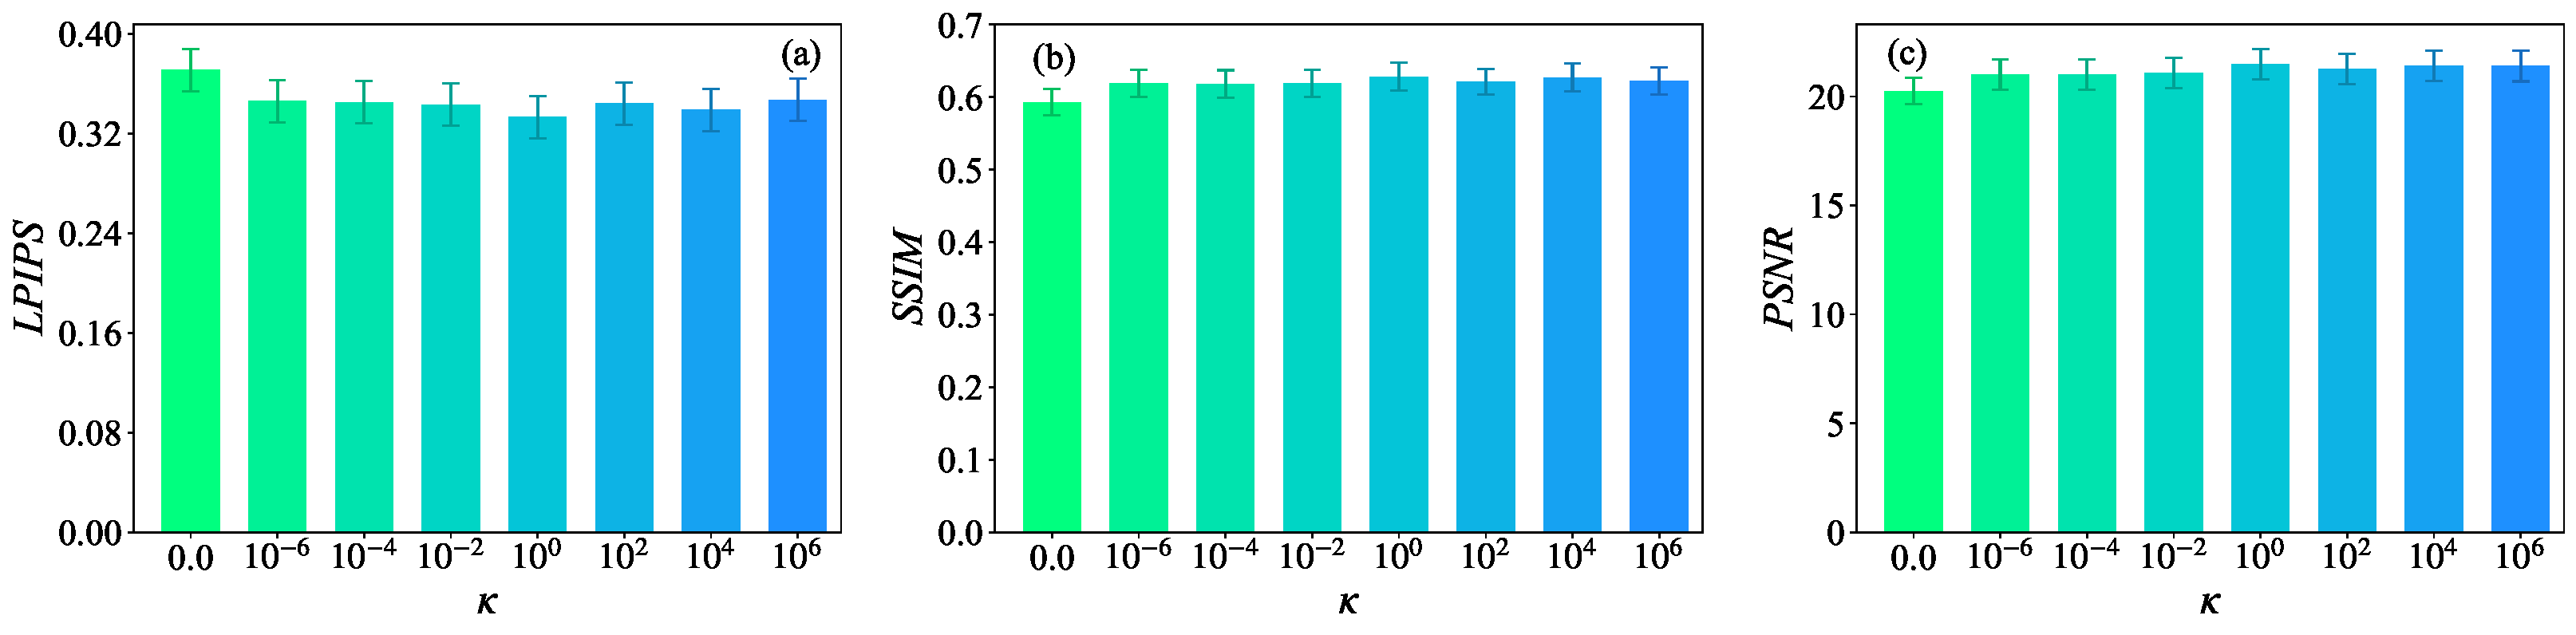
\includegraphics[width=\textwidth]{cvae_celeba_metrics_recon.pdf} 
    \caption{Perceptual and structural reconstruction fidelity of the Coupled Variational Autoencoder (CVAE) across varying coupling parameter ($\kappa$) values. Here we consider image-to-image metrics (LPIPS, SSIM, and PSNR) that strictly evaluate the network's ability to compress and decode individual inputs. The evaluation curves indicate that intermediate heavy-tail coupling (specifically at $\kappa = 10^{0}$) optimizes the latent embedding space, resulting in sharper and structurally superior reconstructions compared to the standard uncoupled Gaussian prior ($\kappa=0$). Even at extreme coupling values ($\kappa \ge 10^2$), the model scores still beats the baseline.}
    \label{fig:metrics_recon}
\end{figure}


\begin{figure}[htbp]
    \centering
    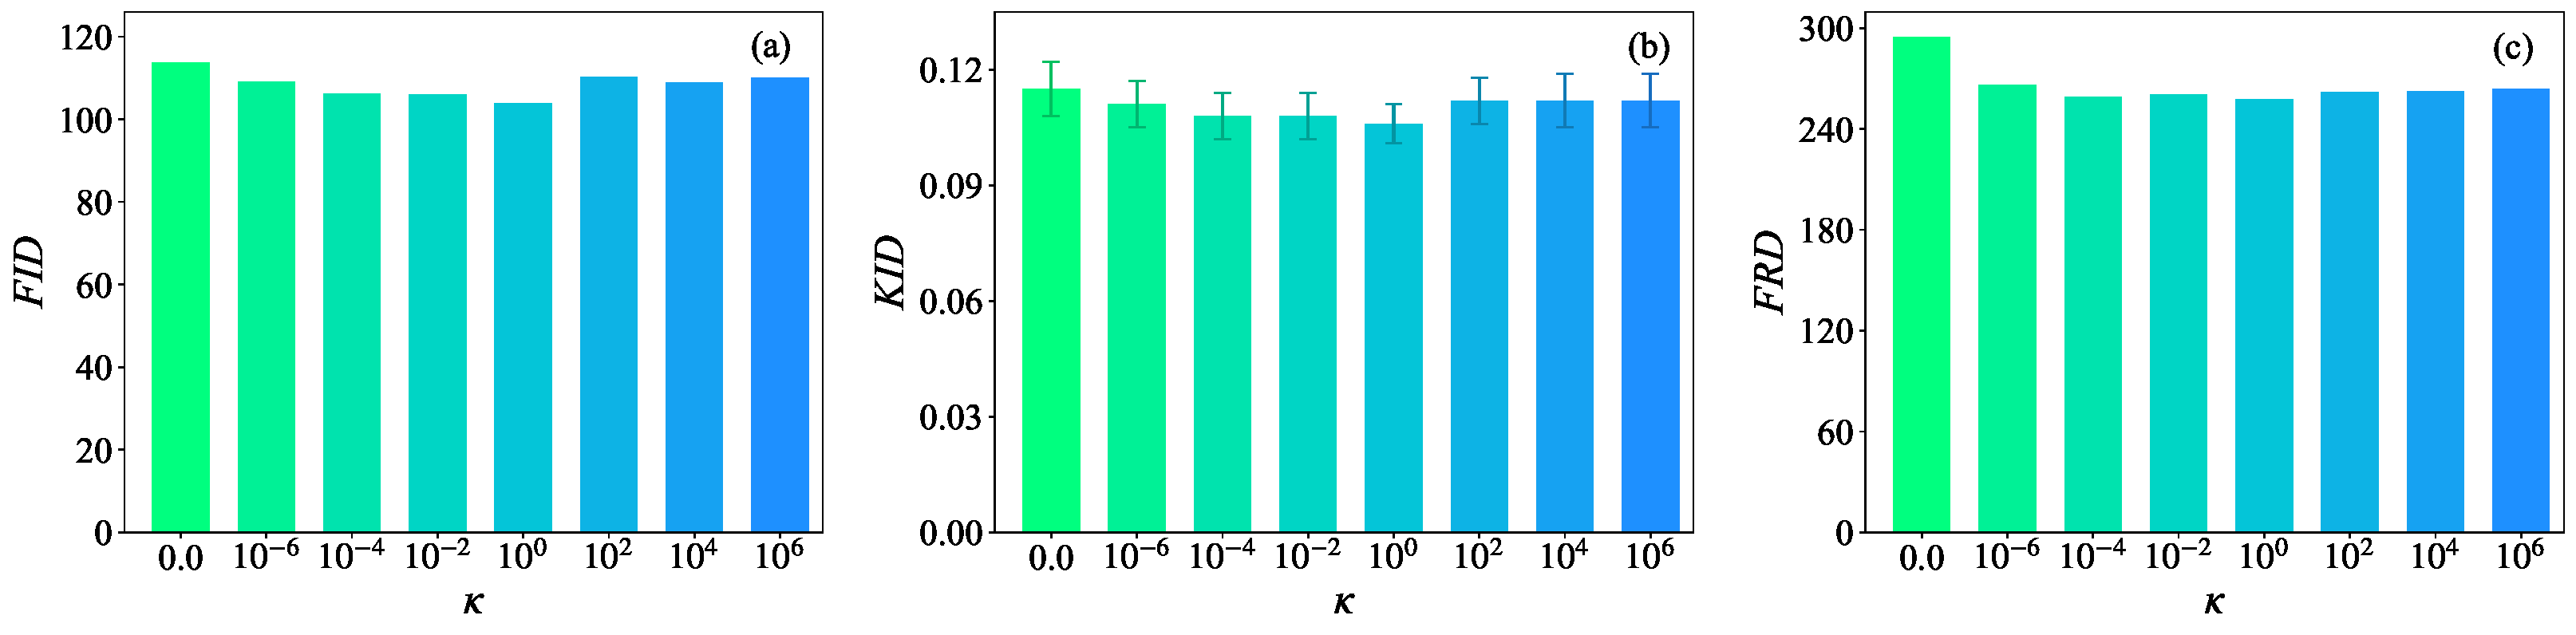
\includegraphics[width=\textwidth]{cvae_celeba_metrics_dist.pdf} 
    \caption{Distributional distance metrics comparing the generated heavy-tail samples against the true dataset manifold over 10,000 evaluations. Fréchet Inception Distance (FID), Kernel Inception Distance (KID), and Fréchet ResNet Distance (FRD) quantify the statistical divergence between deep feature representations. Lower values indicate a closer match to the true data distribution. The results consistently demonstrate that using a latent coupled Normal distribution with a coupling close to 1 ($\kappa \approx 10^{0}$) generates a model that aligns significantly better with the true dataset statistics than the baseline standard Normal distribution ($\kappa = 0$).}
    \label{fig:metrics_dist}
\end{figure}

\begin{figure}[htbp]
    \centering
    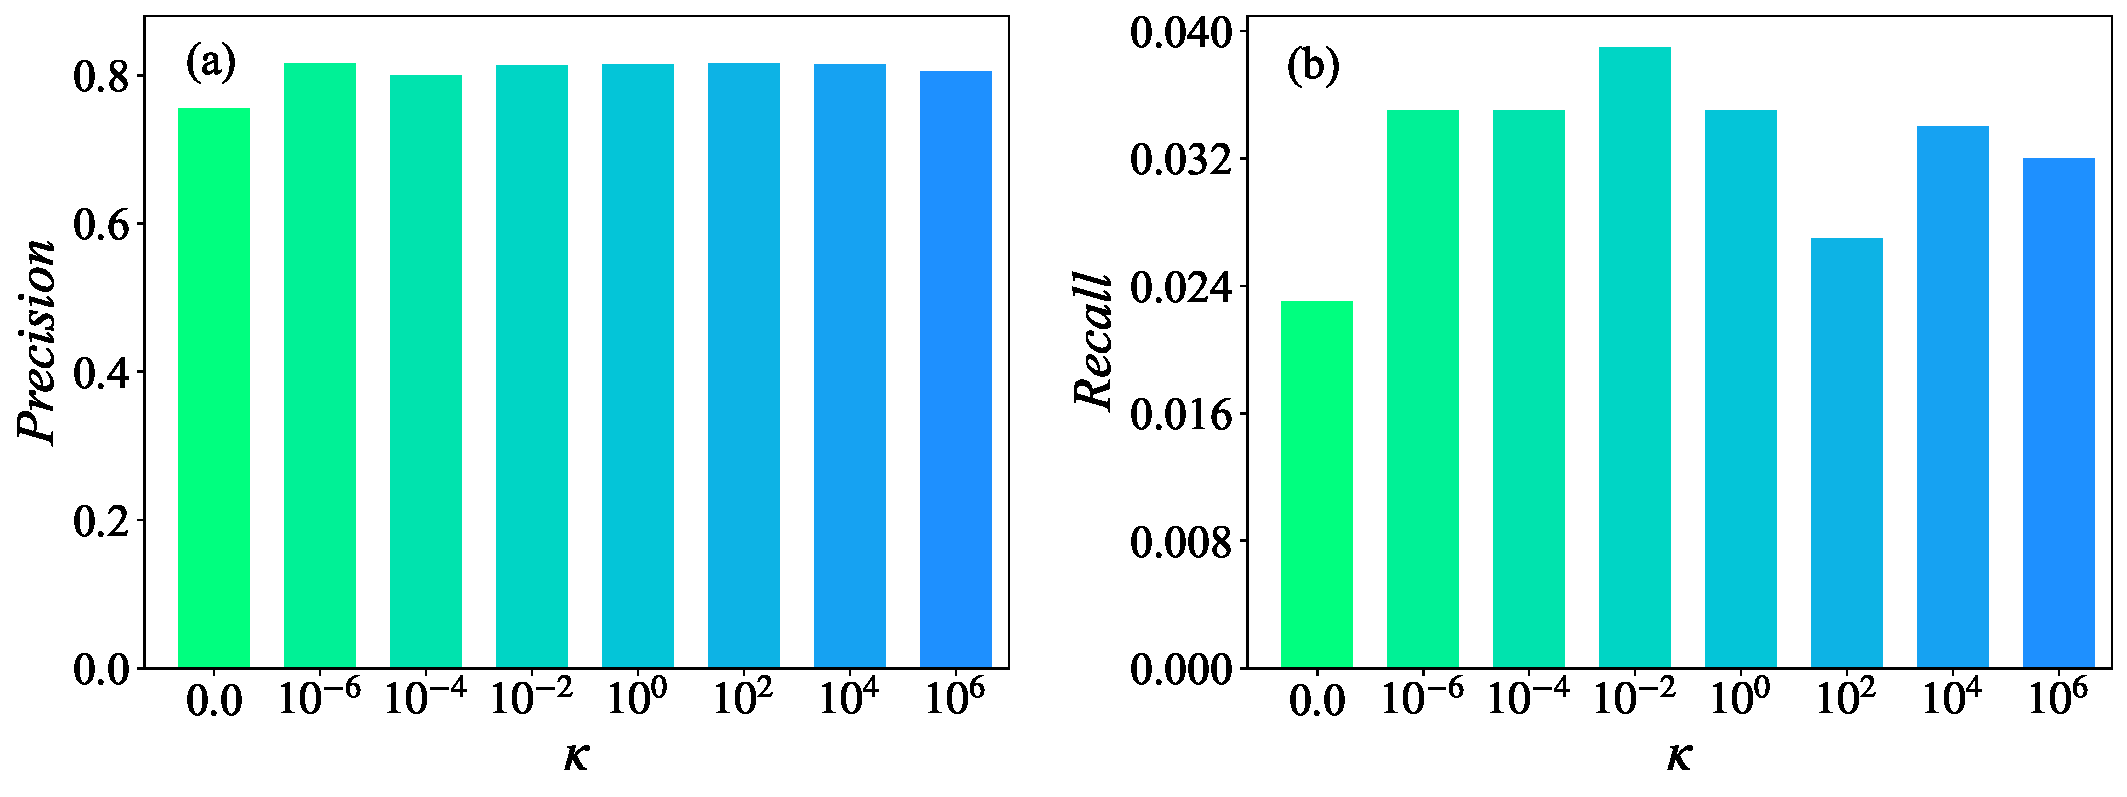
\includegraphics[width=\textwidth]{cvae_celeba_metrics_prec_rec.pdf} 
    \caption{Generative manifold evaluation of the CVAE using k-Nearest Neighbors Precision and Recall. Precision measures the perceptual fidelity of the generated samples (the likelihood that a generated image falls within the real data manifold), while Recall measures mode coverage (the proportion of the real data manifold covered by the generator). The application of a moderate heavy-tail prior ($\kappa = 10^{0}$) yields the highest Precision without sacrificing Recall.}
    \label{fig:metrics_precrec}
\end{figure}

To refine our understanding of the model's peak performance, we conducted a high-resolution ``zoom'' analysis around the optimal coupling value discovered during the initial overview. By focusing on the interval between $\kappa=10^{-2}$ and $\kappa=10^{2}$, we aim to pinpoint the precise non-equilibrium scaling that maximizes generative fidelity and coverage. 

Table \ref{tab:metrics_absolute_zoom} presents the absolute scores for this focused parameter sweep. Rather than a single sharp peak, the high-resolution data reveals a stable performance plateau stretching between $\kappa = 10^{-1}$ and $\kappa = 10^{0}$. Across this regime, the CVAE is consistently able to separate the known deterministic structure from the unknown tail-risk fluctuations. 

Table \ref{tab:metrics_improvement_zoom} details the relative percentage improvements across this zoomed-in domain. The plateau demonstrates a slight trade-off depending on the chosen metric. While $\kappa = 10^{0}$ achieves the optimal Fréchet Inception Distance (9\% improvement) and perceptual similarity (10\% improvement), setting the coupling to $\kappa = 10^{-1}$ yields the strongest structural distribution matching (a 13\% improvement in FRD) and the highest K-NN Precision (a 9\% gain over the baseline). This analysis confirms that tuning the coupling to the mild heavy-tailed domain ($0.1 \le \kappa \le 1.0$) explicitly optimizes the latent embedding space, securing the best overall equilibrium of visual sharpness and topological diversity.

\begin{table}[h!]
\centering
\renewcommand{\arraystretch}{1.4}
\setlength{\tabcolsep}{6pt}
\small
\begin{tabular}{lcccccccc}
\toprule
\rowcolor{gray!20}
\textbf{$\kappa$} & \textbf{FID} & \textbf{KID} & \textbf{LPIPS} & \textbf{SSIM} & \textbf{PSNR} & \textbf{FRD} & \textbf{Prec} & \textbf{Rec} \\
\midrule
$10^{-2}$    & \textcolor{blue}{106.1} & \textcolor{blue}{0.108(6)} & \textcolor{blue}{0.34(2)} & \textcolor{blue}{0.62(2)} & \textcolor{blue}{21.1(7)} & \textcolor{blue}{261} & \textcolor{blue}{0.813} & \textbf{\textcolor{green!50!black}{0.039}} \\
$10^{-1.5}$  & \textcolor{blue}{105.5} & \textcolor{blue}{0.108(7)} & \textcolor{blue}{0.34(2)} & \textbf{\textcolor{green!50!black}{0.63(2)}} & \textcolor{blue}{21.3(7)} & \textcolor{blue}{261} & \textcolor{blue}{0.818} & \textcolor{blue}{0.036} \\
$10^{-1}$    & \textcolor{blue}{104.4} & \textbf{\textcolor{green!50!black}{0.106(6)}} & \textbf{\textcolor{green!50!black}{0.33(2)}} & \textbf{\textcolor{green!50!black}{0.63(2)}} & \textbf{\textcolor{green!50!black}{21.5(7)}} & \textbf{\textcolor{green!50!black}{257}} & \textbf{\textcolor{green!50!black}{0.824}} & \textcolor{blue}{0.035} \\
$10^{-0.5}$  & \textcolor{blue}{105.0} & \textbf{\textcolor{green!50!black}{0.106(6)}} & \textbf{\textcolor{green!50!black}{0.33(2)}} & \textbf{\textcolor{green!50!black}{0.63(2)}} & \textbf{\textcolor{green!50!black}{21.5(7)}} & \textcolor{blue}{258} & \textcolor{blue}{0.812} & \textcolor{blue}{0.037} \\
$10^{0}$     & \textbf{\textcolor{green!50!black}{104.0}} & \textbf{\textcolor{green!50!black}{0.106(5)}} & \textbf{\textcolor{green!50!black}{0.33(2)}} & \textbf{\textcolor{green!50!black}{0.63(2)}} & \textbf{\textcolor{green!50!black}{21.5(7)}} & \textcolor{blue}{258} & \textcolor{blue}{0.815} & \textcolor{blue}{0.035} \\
$10^{0.5}$   & \textcolor{blue}{105.8} & \textcolor{blue}{0.110(6)} & \textbf{\textcolor{green!50!black}{0.33(2)}} & \textbf{\textcolor{green!50!black}{0.63(2)}} & \textbf{\textcolor{green!50!black}{21.5(7)}} & \textcolor{blue}{260} & \textcolor{blue}{0.820} & \textcolor{blue}{0.036} \\
$10^{1}$     & \textcolor{blue}{106.9} & \textcolor{blue}{0.109(6)} & \textcolor{blue}{0.34(2)} & \textbf{\textcolor{green!50!black}{0.63(2)}} & \textbf{\textcolor{green!50!black}{21.5(7)}} & \textcolor{blue}{261} & \textbf{\textcolor{green!50!black}{0.824}} & \textcolor{blue}{0.033} \\
$10^{1.5}$   & \textcolor{blue}{109.9} & \textcolor{blue}{0.113(6)} & \textcolor{blue}{0.34(2)} & \textcolor{blue}{0.62(2)} & \textcolor{blue}{21.4(7)} & \textcolor{blue}{260} & \textcolor{blue}{0.806} & \textcolor{blue}{0.026} \\
$10^{2}$     & \textcolor{blue}{110.3} & \textcolor{blue}{0.112(6)} & \textcolor{blue}{0.34(2)} & \textcolor{blue}{0.62(2)} & \textcolor{blue}{21.3(7)} & \textcolor{blue}{262} & \textcolor{blue}{0.816} & \textcolor{blue}{0.027} \\
\bottomrule
\end{tabular}
\caption{High-resolution evaluation of reconstruction quality for coupling values zoomed around the optimal threshold. The baseline reference remains $\kappa = 0$. Values highlighted in \textcolor{blue}{blue} indicate performance superior to the baseline, while the best overall result for each metric is highlighted in \textbf{\textcolor{green!50!black}{bold green}}. Statistical standard errors are rigorously formatted to one significant digit. FID, FRD, Precision, and Recall are absolute measurements over the entire feature space manifold and do not carry batch-wise variances. A stable plateau of peak performance emerges between $\kappa = 10^{-1}$ and $\kappa = 10^0$, reflecting an optimal separation between the linear scale and nonlinear tail structures.} 
\label{tab:metrics_absolute_zoom}
\end{table}

\begin{table}[h!]
\centering
\renewcommand{\arraystretch}{1.4}
\setlength{\tabcolsep}{6pt}
\small
\begin{tabular}{lcccccccc}
\toprule
\rowcolor{gray!20}
\textbf{$\kappa$} & \textbf{FID} & \textbf{KID} & \textbf{LPIPS} & \textbf{SSIM} & \textbf{PSNR} & \textbf{FRD} & \textbf{Prec} & \textbf{Rec} \\
\midrule
$10^{-2}$    & \textcolor{blue}{6.7\%} & \textcolor{blue}{6(8)\%} & \textcolor{blue}{8(6)\%} & \textcolor{blue}{4(4)\%} & \textcolor{blue}{4(5)\%} & \textcolor{blue}{11.7\%} & \textcolor{blue}{7.7\%} & \textbf{\textcolor{green!50!black}{69.6\%}} \\
$10^{-1.5}$  & \textcolor{blue}{7.2\%} & \textcolor{blue}{6(8)\%} & \textcolor{blue}{9(6)\%} & \textcolor{blue}{5(4)\%} & \textcolor{blue}{5(5)\%} & \textcolor{blue}{11.4\%} & \textcolor{blue}{8.3\%} & \textcolor{blue}{56.5\%} \\
$10^{-1}$    & \textcolor{blue}{8.1\%} & \textbf{\textcolor{green!50!black}{8(8)\%}} & \textbf{\textcolor{green!50!black}{10(6)\%}} & \textbf{\textcolor{green!50!black}{6(5)\%}} & \textbf{\textcolor{green!50!black}{6(5)\%}} & \textbf{\textcolor{green!50!black}{12.9\%}} & \textbf{\textcolor{green!50!black}{9.1\%}} & \textcolor{blue}{52.2\%} \\
$10^{-0.5}$  & \textcolor{blue}{7.6\%} & \textbf{\textcolor{green!50!black}{8(8)\%}} & \textbf{\textcolor{green!50!black}{10(6)\%}} & \textbf{\textcolor{green!50!black}{6(5)\%}} & \textbf{\textcolor{green!50!black}{6(5)\%}} & \textcolor{blue}{12.7\%} & \textcolor{blue}{7.5\%} & \textcolor{blue}{60.9\%} \\
$10^{0}$     & \textbf{\textcolor{green!50!black}{8.5\%}} & \textbf{\textcolor{green!50!black}{8(8)\%}} & \textbf{\textcolor{green!50!black}{10(6)\%}} & \textcolor{blue}{5(4)\%} & \textbf{\textcolor{green!50!black}{6(5)\%}} & \textcolor{blue}{12.6\%} & \textcolor{blue}{7.9\%} & \textcolor{blue}{52.2\%} \\
$10^{0.5}$   & \textcolor{blue}{6.9\%} & \textcolor{blue}{4(8)\%} & \textbf{\textcolor{green!50!black}{10(6)\%}} & \textcolor{blue}{5(4)\%} & \textbf{\textcolor{green!50!black}{6(5)\%}} & \textcolor{blue}{11.8\%} & \textcolor{blue}{8.6\%} & \textcolor{blue}{56.5\%} \\
$10^{1}$     & \textcolor{blue}{5.9\%} & \textcolor{blue}{5(8)\%} & \textcolor{blue}{9(6)\%} & \textcolor{blue}{5(4)\%} & \textbf{\textcolor{green!50!black}{6(5)\%}} & \textcolor{blue}{11.4\%} & \textbf{\textcolor{green!50!black}{9.1\%}} & \textcolor{blue}{43.5\%} \\
$10^{1.5}$   & \textcolor{blue}{3.3\%} & \textcolor{blue}{1(8)\%} & \textcolor{blue}{8(6)\%} & \textcolor{blue}{5(4)\%} & \textcolor{blue}{5(5)\%} & \textcolor{blue}{11.9\%} & \textcolor{blue}{6.8\%} & \textcolor{blue}{13.0\%} \\
$10^{2}$     & \textcolor{blue}{3.0\%} & \textcolor{blue}{2(7)\%} & \textcolor{blue}{7(6)\%} & \textcolor{blue}{4(4)\%} & \textcolor{blue}{5(5)\%} & \textcolor{blue}{11.3\%} & \textcolor{blue}{8.1\%} & \textcolor{blue}{17.4\%} \\
\bottomrule
\end{tabular}
\caption{Relative percentage improvement for the zoomed coupling interval compared to the standard Gaussian baseline ($\kappa = 0$). Propagated standard errors are provided in parentheses where variance is mathematically defined. Values in \textcolor{blue}{blue} signify positive gains, and \textbf{\textcolor{green!50!black}{bold green}} indicates the maximum improvement observed. The analysis confirms a strong generative performance plateau encompassing both $\kappa = 10^{-1}$ and $\kappa = 10^0$, reflecting optimized structural representation and dataset coverage before the heavy-tailed regularization becomes overly rigid.}
\label{tab:metrics_improvement_zoom}
\end{table}

\subsection{CVAE Robustness and Denoising Capability}

To evaluate the resilience of the generated latent space, we designed an experiment to test the model's capacity to recover structural information from degraded inputs. We applied four distinct types of image corruption to the original 10,000 evaluation images including additive Gaussian noise, motion blur, Poisson shot noise, and simulated fog. We then passed these corrupted images through the pre-trained models. The resulting reconstructions were evaluated against the clean original images rather than the corrupted inputs. This approach ensures the metrics reward structural recovery and penalize the mere memorization of applied noise.

Tables \ref{tab:robustness_gaussian_abs} through \ref{tab:robustness_fog_abs} present the absolute scores for each degradation type, while Tables \ref{tab:robustness_gaussian_rel} through \ref{tab:robustness_fog_rel} display the relative percentage improvements over the standard Gaussian baseline ($\kappa = 0$). 

The data reveals that the optimal configuration remains consistent. The model with $\kappa = 10^0$ continues to yield the best overall balance of visual fidelity and distribution alignment across all corruption types. This confirms that a moderate heavy tail is universally beneficial for structuring the latent space, rather than being an artifact of clean data. 

Comparing the different corruptions provides clear physical insights. Additive Gaussian noise was the easiest to mitigate. Because this noise is symmetric and random, the model easily filtered it out, achieving scores (e.g., FID of 104.4) nearly identical to the uncorrupted baseline tests. In contrast, simulated fog was the most difficult. Fog acts as a global occlusion, removing contrast and structural edges. Rather than simply perturbing the data, it erases it, causing overall metrics to drop significantly across all models (e.g., PSNR falling to ~11.7). Motion blur and Poisson shot noise sit in the middle. These corruptions hold high practical importance, as they represent the physical constraints of real-world sensors operating in low-light environments or on moving platforms like vehicles and satellites.

The relative tables show that while severe corruptions lower the absolute scores, the relative advantage of the CVAE over the standard model remains strong. The mechanism behind this denoising capability relies on the shape of the prior distribution. A standard baseline model forces all data into a strict, narrow bell curve. When it encounters heavy noise, it treats those extreme pixel variations as important features, causing the encoded representation to shift, which leads the decoder to reproduce the noise. 

The heavy-tailed prior of the CVAE acts as a statistical shock absorber. Due to the independent-equals expectation, the model anticipates large deviations. It allows the noise to sit harmlessly in the broad tails of the distribution without pulling the core structural embedding off-center. Consequently, the decoder ignores the random noise and reconstructs only the central structural features of the underlying face.

% ==========================================
% GAUSSIAN NOISE TABLES
% ==========================================
\begin{table}[h!]
\centering
\renewcommand{\arraystretch}{1.4}
\setlength{\tabcolsep}{6pt}
\small
\begin{tabular}{lcccccccc}
\toprule
\rowcolor{gray!20}
\multicolumn{9}{c}{\textbf{Additive Gaussian Noise - Absolute Scores}} \\
\textbf{$\kappa$} & \textbf{FID} & \textbf{KID} & \textbf{LPIPS} & \textbf{SSIM} & \textbf{PSNR} & \textbf{FRD} & \textbf{Prec} & \textbf{Rec} \\
\midrule
$0.0$        & 114.6 & 0.116(7) & 0.38(2) & 0.58(2) & 20.2(3) & 298 & 0.752 & 0.017 \\
$10^{-6}$    & \textcolor{blue}{109.4} & \textcolor{blue}{0.113(6)} & \textcolor{blue}{0.35(2)} & \textcolor{blue}{0.61(2)} & \textcolor{blue}{20.9(3)} & \textcolor{blue}{269} & \textbf{\textcolor{green!50!black}{0.814}} & \textbf{\textcolor{green!50!black}{0.033}} \\
$10^{-4}$    & \textcolor{blue}{106.8} & \textcolor{blue}{0.108(6)} & \textcolor{blue}{0.35(2)} & \textcolor{blue}{0.61(2)} & \textcolor{blue}{20.9(3)} & \textcolor{blue}{264} & \textcolor{blue}{0.792} & \textcolor{blue}{0.032} \\
$10^{-2}$    & \textcolor{blue}{107.0} & \textcolor{blue}{0.109(7)} & \textcolor{blue}{0.35(2)} & \textcolor{blue}{0.61(2)} & \textcolor{blue}{21.0(3)} & \textcolor{blue}{265} & \textcolor{blue}{0.803} & \textcolor{blue}{0.027} \\
$10^{0}$     & \textbf{\textcolor{green!50!black}{104.4}} & \textbf{\textcolor{green!50!black}{0.106(6)}} & \textbf{\textcolor{green!50!black}{0.34(2)}} & \textbf{\textcolor{green!50!black}{0.61(2)}} & \textbf{\textcolor{green!50!black}{21.4(4)}} & \textbf{\textcolor{green!50!black}{262}} & \textcolor{blue}{0.803} & \textbf{\textcolor{green!50!black}{0.033}} \\
$10^{2}$     & \textcolor{blue}{111.4} & \textcolor{blue}{0.112(6)} & \textcolor{blue}{0.35(2)} & \textcolor{blue}{0.61(2)} & \textcolor{blue}{21.2(4)} & \textcolor{blue}{266} & \textcolor{blue}{0.813} & \textcolor{blue}{0.023} \\
$10^{4}$     & \textcolor{blue}{109.5} & \textcolor{blue}{0.111(6)} & \textcolor{blue}{0.34(2)} & \textcolor{blue}{0.61(2)} & \textcolor{blue}{21.3(4)} & \textcolor{blue}{267} & \textcolor{blue}{0.804} & \textcolor{blue}{0.028} \\
$10^{6}$     & \textcolor{blue}{110.3} & \textcolor{blue}{0.112(6)} & \textcolor{blue}{0.35(2)} & \textcolor{blue}{0.61(2)} & \textcolor{blue}{21.3(4)} & \textcolor{blue}{267} & \textcolor{blue}{0.800} & \textcolor{blue}{0.026} \\
\bottomrule
\end{tabular}
\caption{\textcolor{red}{update caption more description}Absolute reconstruction quality evaluated on inputs corrupted with additive Gaussian noise.}
\label{tab:robustness_gaussian_abs}
\end{table}

\begin{table}[h!]
\centering
\renewcommand{\arraystretch}{1.4}
\setlength{\tabcolsep}{6pt}
\small
\begin{tabular}{lcccccccc}
\toprule
\rowcolor{gray!20}
\multicolumn{9}{c}{\textbf{Additive Gaussian Noise - Relative Improvement}} \\
\textbf{$\kappa$} & \textbf{FID} & \textbf{KID} & \textbf{LPIPS} & \textbf{SSIM} & \textbf{PSNR} & \textbf{FRD} & \textbf{Prec} & \textbf{Rec} \\
\midrule
$10^{-6}$    & \textcolor{blue}{5\%} & \textcolor{blue}{3(8)\%} & \textcolor{blue}{7(6)\%} & \textcolor{blue}{4(4)\%} & \textcolor{blue}{4(3)\%} & \textcolor{blue}{10\%} & \textbf{\textcolor{green!50!black}{8\%}} & \textbf{\textcolor{green!50!black}{94\%}} \\
$10^{-4}$    & \textcolor{blue}{7\%} & \textcolor{blue}{7(8)\%} & \textcolor{blue}{7(6)\%} & \textcolor{blue}{4(4)\%} & \textcolor{blue}{4(3)\%} & \textcolor{blue}{11\%} & \textcolor{blue}{5\%} & \textcolor{blue}{88\%} \\
$10^{-2}$    & \textcolor{blue}{7\%} & \textcolor{blue}{6(8)\%} & \textcolor{blue}{7(6)\%} & \textcolor{blue}{4(4)\%} & \textcolor{blue}{4(3)\%} & \textcolor{blue}{11\%} & \textcolor{blue}{7\%} & \textcolor{blue}{59\%} \\
$10^{0}$     & \textbf{\textcolor{green!50!black}{9\%}} & \textbf{\textcolor{green!50!black}{9(8)\%}} & \textbf{\textcolor{green!50!black}{10(6)\%}} & \textbf{\textcolor{green!50!black}{5(4)\%}} & \textbf{\textcolor{green!50!black}{6(2)\%}} & \textbf{\textcolor{green!50!black}{12\%}} & \textcolor{blue}{7\%} & \textbf{\textcolor{green!50!black}{94\%}} \\
$10^{2}$     & \textcolor{blue}{3\%} & \textcolor{blue}{3(7)\%} & \textcolor{blue}{7(6)\%} & \textcolor{blue}{4(4)\%} & \textcolor{blue}{5(3)\%} & \textcolor{blue}{11\%} & \textcolor{blue}{8\%} & \textcolor{blue}{35\%} \\
$10^{4}$     & \textcolor{blue}{4\%} & \textcolor{blue}{4(8)\%} & \textcolor{blue}{8(6)\%} & \textcolor{blue}{5(4)\%} & \textcolor{blue}{6(3)\%} & \textcolor{blue}{10\%} & \textcolor{blue}{7\%} & \textcolor{blue}{65\%} \\
$10^{6}$     & \textcolor{blue}{4\%} & \textcolor{blue}{3(8)\%} & \textcolor{blue}{6(6)\%} & \textcolor{blue}{4(4)\%} & \textcolor{blue}{5(3)\%} & \textcolor{blue}{10\%} & \textcolor{blue}{6\%} & \textcolor{blue}{53\%} \\
\bottomrule
\end{tabular}
\caption{Relative percentage improvement for Gaussian noise compared to the baseline ($\kappa = 0$).}
\label{tab:robustness_gaussian_rel}
\end{table}

% ==========================================
% MOTION BLUR TABLES
% ==========================================
\begin{table}[h!]
\centering
\renewcommand{\arraystretch}{1.4}
\setlength{\tabcolsep}{6pt}
\small
\begin{tabular}{lcccccccc}
\toprule
\rowcolor{gray!20}
\multicolumn{9}{c}{\textbf{Motion Blur - Absolute Scores}} \\
\textbf{$\kappa$} & \textbf{FID} & \textbf{KID} & \textbf{LPIPS} & \textbf{SSIM} & \textbf{PSNR} & \textbf{FRD} & \textbf{Prec} & \textbf{Rec} \\
\midrule
$0.0$        & 123.7 & 0.126(7) & 0.41(2) & 0.56(1) & 18.9(3) & 345 & 0.695 & 0.008 \\
$10^{-6}$    & \textcolor{blue}{120.8} & \textcolor{blue}{0.125(6)} & \textcolor{blue}{0.39(2)} & \textcolor{blue}{0.58(2)} & \textcolor{blue}{19.6(3)} & \textcolor{blue}{315} & \textcolor{blue}{0.734} & \textcolor{blue}{0.013} \\
$10^{-4}$    & \textcolor{blue}{117.6} & \textcolor{blue}{0.121(5)} & \textcolor{blue}{0.39(2)} & \textcolor{blue}{0.58(2)} & \textcolor{blue}{19.5(3)} & \textcolor{blue}{310} & \textcolor{blue}{0.735} & \textbf{\textcolor{green!50!black}{0.016}} \\
$10^{-2}$    & \textcolor{blue}{116.9} & \textcolor{blue}{0.119(7)} & \textcolor{blue}{0.39(2)} & \textcolor{blue}{0.58(2)} & \textcolor{blue}{19.6(3)} & \textcolor{blue}{310} & \textcolor{blue}{0.740} & \textcolor{blue}{0.013} \\
$10^{0}$     & \textbf{\textcolor{green!50!black}{116.4}} & \textbf{\textcolor{green!50!black}{0.120(6)}} & \textbf{\textcolor{green!50!black}{0.38(2)}} & \textbf{\textcolor{green!50!black}{0.58(2)}} & \textbf{\textcolor{green!50!black}{19.9(3)}} & \textbf{\textcolor{green!50!black}{307}} & \textcolor{blue}{0.742} & \textcolor{blue}{0.012} \\
$10^{2}$     & \textcolor{blue}{122.7} & \textcolor{blue}{0.126(7)} & \textcolor{blue}{0.39(2)} & \textcolor{blue}{0.58(2)} & \textcolor{blue}{19.7(3)} & \textcolor{blue}{308} & \textcolor{blue}{0.756} & \textcolor{blue}{0.009} \\
$10^{4}$     & \textcolor{blue}{119.8} & \textcolor{blue}{0.122(6)} & \textbf{\textcolor{green!50!black}{0.38(2)}} & \textbf{\textcolor{green!50!black}{0.59(2)}} & \textcolor{blue}{19.9(3)} & \textcolor{blue}{313} & \textbf{\textcolor{green!50!black}{0.757}} & \textcolor{blue}{0.012} \\
$10^{6}$     & \textcolor{blue}{120.7} & \textcolor{blue}{0.123(6)} & \textcolor{blue}{0.39(1)} & \textcolor{blue}{0.58(2)} & \textcolor{blue}{19.9(3)} & \textcolor{blue}{313} & \textcolor{blue}{0.754} & \textcolor{blue}{0.010} \\
\bottomrule
\end{tabular}
\caption{Absolute reconstruction quality evaluated on inputs corrupted with directional motion blur.}
\label{tab:robustness_motion_blur_abs}
\end{table}

\begin{table}[h!]
\centering
\renewcommand{\arraystretch}{1.4}
\setlength{\tabcolsep}{6pt}
\small
\begin{tabular}{lcccccccc}
\toprule
\rowcolor{gray!20}
\multicolumn{9}{c}{\textbf{Motion Blur - Relative Improvement}} \\
\textbf{$\kappa$} & \textbf{FID} & \textbf{KID} & \textbf{LPIPS} & \textbf{SSIM} & \textbf{PSNR} & \textbf{FRD} & \textbf{Prec} & \textbf{Rec} \\
\midrule
$10^{-6}$    & \textcolor{blue}{2\%} & \textcolor{blue}{1(8)\%} & \textcolor{blue}{4(6)\%} & \textcolor{blue}{4(3)\%} & \textcolor{blue}{4(2)\%} & \textcolor{blue}{9\%} & \textcolor{blue}{6\%} & \textcolor{blue}{63\%} \\
$10^{-4}$    & \textcolor{blue}{5\%} & \textcolor{blue}{4(7)\%} & \textcolor{blue}{4(6)\%} & \textcolor{blue}{4(3)\%} & \textcolor{blue}{3(2)\%} & \textcolor{blue}{10\%} & \textcolor{blue}{6\%} & \textbf{\textcolor{green!50!black}{100\%}} \\
$10^{-2}$    & \textcolor{blue}{5\%} & \textcolor{blue}{5(8)\%} & \textcolor{blue}{5(6)\%} & \textcolor{blue}{4(3)\%} & \textcolor{blue}{4(2)\%} & \textcolor{blue}{10\%} & \textcolor{blue}{6\%} & \textcolor{blue}{63\%}  \\
$10^{0}$     & \textbf{\textcolor{green!50!black}{6\%}} & \textbf{\textcolor{green!50!black}{5(8)\%}} & \textbf{\textcolor{green!50!black}{6(6)\%}} & \textbf{\textcolor{green!50!black}{5(3)\%}} & \textbf{\textcolor{green!50!black}{5(2)\%}} & \textbf{\textcolor{green!50!black}{11\%}} & \textcolor{blue}{7\%} & \textcolor{blue}{50\%} \\
$10^{2}$     & \textcolor{blue}{1\%} & \textcolor{blue}{0(7)\%} & \textcolor{blue}{5(6)\%} & \textcolor{blue}{4(3)\%} & \textcolor{blue}{4(2)\%} & \textcolor{blue}{11\%} & \textcolor{blue}{9\%} & \textcolor{blue}{13\%} \\
$10^{4}$     & \textcolor{blue}{3\%} & \textcolor{blue}{3(8)\%} & \textbf{\textcolor{green!50!black}{6(6)\%}} & \textbf{\textcolor{green!50!black}{5(3)\%}} & \textcolor{blue}{5(2)\%} & \textcolor{blue}{9\%} & \textbf{\textcolor{green!50!black}{9\%}} & \textcolor{blue}{50\%} \\
$10^{6}$     & \textcolor{blue}{2\%} & \textcolor{blue}{2(8)\%} & \textcolor{blue}{4(5)\%} & \textcolor{blue}{4(3)\%} & \textcolor{blue}{5(2)\%} & \textcolor{blue}{9\%} & \textcolor{blue}{8\%} & \textcolor{blue}{25\%} \\
\bottomrule
\end{tabular}
\caption{Relative percentage improvement for motion blur compared to the baseline ($\kappa = 0$).}
\label{tab:robustness_motion_blur_rel}
\end{table}

% ==========================================
% SHOT NOISE TABLES
% ==========================================
\begin{table}[h!]
\centering
\renewcommand{\arraystretch}{1.4}
\setlength{\tabcolsep}{6pt}
\small
\begin{tabular}{lcccccccc}
\toprule
\rowcolor{gray!20}
\multicolumn{9}{c}{\textbf{Poisson Shot Noise - Absolute Scores}} \\
\textbf{$\kappa$} & \textbf{FID} & \textbf{KID} & \textbf{LPIPS} & \textbf{SSIM} & \textbf{PSNR} & \textbf{FRD} & \textbf{Prec} & \textbf{Rec} \\
\midrule
$0.0$        & 122.7 & 0.125(7) & 0.43(2) & 0.54(1) & 15.3(3) & 379 & 0.614 & 0.006 \\
$10^{-6}$    & \textcolor{blue}{115.2} & \textcolor{blue}{0.119(7)} & \textcolor{blue}{0.40(2)} & \textcolor{blue}{0.57(2)} & \textcolor{blue}{15.8(3)} & \textcolor{blue}{328} & \textbf{\textcolor{green!50!black}{0.715}} & \textcolor{blue}{0.009} \\
$10^{-4}$    & \textcolor{blue}{113.3} & \textcolor{blue}{0.115(7)} & \textcolor{blue}{0.40(2)} & \textcolor{blue}{0.57(2)} & \textcolor{blue}{15.7(3)} & \textcolor{blue}{333} & \textcolor{blue}{0.683} & \textcolor{blue}{0.010} \\
$10^{-2}$    & \textcolor{blue}{112.2} & \textcolor{blue}{0.114(6)} & \textcolor{blue}{0.40(2)} & \textcolor{blue}{0.57(2)} & \textcolor{blue}{15.6(3)} & \textcolor{blue}{329} & \textcolor{blue}{0.709} & \textbf{\textcolor{green!50!black}{0.013}} \\
$10^{0}$     & \textbf{\textcolor{green!50!black}{111.3}} & \textbf{\textcolor{green!50!black}{0.113(6)}} & \textbf{\textcolor{green!50!black}{0.38(2)}} & \textbf{\textcolor{green!50!black}{0.58(2)}} & \textcolor{blue}{15.8(3)} & \textbf{\textcolor{green!50!black}{326}} & \textcolor{blue}{0.702} & \textbf{\textcolor{green!50!black}{0.013}} \\
$10^{2}$     & \textcolor{blue}{117.6} & \textcolor{blue}{0.120(6)} & \textcolor{blue}{0.40(2)} & \textcolor{blue}{0.58(2)} & \textcolor{blue}{15.6(3)} & \textcolor{blue}{329} & \textcolor{blue}{0.705} & \textcolor{blue}{0.009} \\
$10^{4}$     & \textcolor{blue}{116.0} & \textcolor{blue}{0.119(6)} & \textcolor{blue}{0.39(2)} & \textcolor{blue}{0.58(2)} & \textcolor{blue}{15.7(3)} & \textcolor{blue}{334} & \textcolor{blue}{0.693} & \textcolor{blue}{0.009} \\
$10^{6}$     & \textcolor{blue}{116.2} & \textcolor{blue}{0.118(7)} & \textcolor{blue}{0.41(2)} & \textcolor{blue}{0.58(2)} & \textbf{\textcolor{green!50!black}{15.9(3)}} & \textcolor{blue}{325} & \textcolor{blue}{0.711} & \textcolor{blue}{0.008} \\
\bottomrule
\end{tabular}
\caption{Absolute reconstruction quality evaluated on inputs corrupted with Poisson shot noise.}
\label{tab:robustness_shot_noise_abs}
\end{table}

\begin{table}[h!]
\centering
\renewcommand{\arraystretch}{1.4}
\setlength{\tabcolsep}{6pt}
\small
\begin{tabular}{lcccccccc}
\toprule
\rowcolor{gray!20}
\multicolumn{9}{c}{\textbf{Poisson Shot Noise - Relative Improvement}} \\
\textbf{$\kappa$} & \textbf{FID} & \textbf{KID} & \textbf{LPIPS} & \textbf{SSIM} & \textbf{PSNR} & \textbf{FRD} & \textbf{Prec} & \textbf{Rec} \\
\midrule
$10^{-6}$    & \textcolor{blue}{6\%} & \textcolor{blue}{5(8)\%} & \textcolor{blue}{7(6)\%} & \textcolor{blue}{6(4)\%} & \textcolor{blue}{3(3)\%} & \textcolor{blue}{13\%} & \textbf{\textcolor{green!50!black}{16\%}} & \textcolor{blue}{50\%} \\
$10^{-4}$    & \textcolor{blue}{8\%} & \textcolor{blue}{8(8)\%} & \textcolor{blue}{6(6)\%} & \textcolor{blue}{6(4)\%} & \textcolor{blue}{3(3)\%} & \textcolor{blue}{12\%} & \textcolor{blue}{11\%} & \textcolor{blue}{67\%} \\
$10^{-2}$    & \textcolor{blue}{9\%} & \textcolor{blue}{9(8)\%} & \textcolor{blue}{7(6)\%} & \textcolor{blue}{6(4)\%} & \textcolor{blue}{2(3)\%} & \textcolor{blue}{13\%} & \textcolor{blue}{15\%} & \textbf{\textcolor{green!50!black}{117\%}} \\
$10^{0}$     & \textbf{\textcolor{green!50!black}{9\%}} & \textbf{\textcolor{green!50!black}{10(8)\%}} & \textbf{\textcolor{green!50!black}{10(6)\%}} & \textbf{\textcolor{green!50!black}{8(4)\%}} & \textcolor{blue}{4(3)\%} & \textbf{\textcolor{green!50!black}{14\%}} & \textcolor{blue}{14\%} & \textbf{\textcolor{green!50!black}{117\%}} \\
$10^{2}$     & \textcolor{blue}{4\%} & \textcolor{blue}{4(8)\%} & \textcolor{blue}{7(6)\%} & \textcolor{blue}{7(4)\%} & \textcolor{blue}{2(3)\%} & \textcolor{blue}{13\%} & \textcolor{blue}{15\%} & \textcolor{blue}{50\%} \\
$10^{4}$     & \textcolor{blue}{5\%} & \textcolor{blue}{5(8)\%} & \textcolor{blue}{8(6)\%} & \textcolor{blue}{7(4)\%} & \textcolor{blue}{3(3)\%} & \textcolor{blue}{12\%} & \textcolor{blue}{13\%} & \textcolor{blue}{50\%} \\
$10^{6}$     & \textcolor{blue}{5\%} & \textcolor{blue}{6(8)\%} & \textcolor{blue}{4(6)\%} & \textcolor{blue}{7(4)\%} & \textbf{\textcolor{green!50!black}{4(3)\%}} & \textcolor{blue}{14\%} & \textcolor{blue}{16\%} & \textcolor{blue}{33\%} \\
\bottomrule
\end{tabular}
\caption{Relative percentage improvement for shot noise compared to the baseline ($\kappa = 0$).}
\label{tab:robustness_shot_noise_rel}
\end{table}

% ==========================================
% FOG TABLES
% ==========================================
\begin{table}[h!]
\centering
\renewcommand{\arraystretch}{1.4}
\setlength{\tabcolsep}{6pt}
\small
\begin{tabular}{lcccccccc}
\toprule
\rowcolor{gray!20}
\multicolumn{9}{c}{\textbf{Simulated Fog - Absolute Scores}} \\
\textbf{$\kappa$} & \textbf{FID} & \textbf{KID} & \textbf{LPIPS} & \textbf{SSIM} & \textbf{PSNR} & \textbf{FRD} & \textbf{Prec} & \textbf{Rec} \\
\midrule
$0.0$        & 167.7 & 0.186(8) & 0.54(2) & 0.40(2) & 11.7(3) & 459 & 0.620 & 0.000 \\
$10^{-6}$    & \textcolor{blue}{160.0} & \textcolor{blue}{0.174(9)} & \textcolor{blue}{0.53(2)} & \textcolor{blue}{0.41(2)} & 11.5(3) & \textcolor{blue}{431} & \textcolor{blue}{0.648} & \textcolor{blue}{0.001}  \\
$10^{-4}$    & \textcolor{blue}{158.1} & \textcolor{blue}{0.172(8)} & \textcolor{blue}{0.53(2)} & \textcolor{blue}{0.41(2)} & 11.6(3) & \textcolor{blue}{430} & \textcolor{blue}{0.632} & \textbf{\textcolor{green!50!black}{0.004}} \\
$10^{-2}$    & \textcolor{blue}{159.7} & \textcolor{blue}{0.176(9)} & \textcolor{blue}{0.52(2)} & \textcolor{blue}{0.42(2)} & 11.7(3) & \textbf{\textcolor{green!50!black}{417}} & \textbf{\textcolor{green!50!black}{0.666}} & 0.000 \\
$10^{0}$     & \textbf{\textcolor{green!50!black}{157.6}} & \textbf{\textcolor{green!50!black}{0.175(8)}} & \textbf{\textcolor{green!50!black}{0.52(2)}} & \textbf{\textcolor{green!50!black}{0.42(2)}} & \textbf{\textcolor{green!50!black}{11.7(3)}} & \textcolor{blue}{436} & 0.617 & 0.000 \\
$10^{2}$     & \textcolor{blue}{166.0} & \textcolor{blue}{0.182(9)} & \textcolor{blue}{0.54(2)} & \textcolor{blue}{0.41(2)} & \textcolor{blue}{11.8(3)} & \textcolor{blue}{445} & \textcolor{blue}{0.628} & 0.000 \\
$10^{4}$     & \textcolor{blue}{163.6} & \textcolor{blue}{0.181(9)} & \textcolor{blue}{0.53(2)} & \textcolor{blue}{0.42(2)} & \textcolor{blue}{11.8(3)} & \textcolor{blue}{435} & \textcolor{blue}{0.629} & 0.000 \\
$10^{6}$     & \textcolor{blue}{165.7} & \textcolor{blue}{0.181(9)} & \textcolor{blue}{0.53(2)} & \textcolor{blue}{0.41(2)} & 11.6(3) & \textcolor{blue}{439} & \textcolor{blue}{0.633} & 0.000 \\
\bottomrule
\end{tabular}
\caption{Absolute reconstruction quality evaluated on inputs corrupted with dense, simulated fog.}
\label{tab:robustness_fog_abs}
\end{table}

\begin{table}[h!]
\centering
\renewcommand{\arraystretch}{1.4}
\setlength{\tabcolsep}{6pt}
\small
\begin{tabular}{lcccccccc}
\toprule
\rowcolor{gray!20}
\multicolumn{9}{c}{\textbf{Simulated Fog - Relative Improvement}} \\
\textbf{$\kappa$} & \textbf{FID} & \textbf{KID} & \textbf{LPIPS} & \textbf{SSIM} & \textbf{PSNR} & \textbf{FRD} & \textbf{Prec} & \textbf{Rec} \\
\midrule
$10^{-6}$    & \textcolor{blue}{5\%} & \textcolor{blue}{6(8)\%} & \textcolor{blue}{2(5)\%} & \textcolor{blue}{2(7)\%} & -2(4)\% & \textcolor{blue}{6\%} & \textcolor{blue}{5\%} & \textbf{\textcolor{green!50!black}{--}} \\
$10^{-4}$    & \textcolor{blue}{6\%} & \textcolor{blue}{8(8)\%} & \textcolor{blue}{2(5)\%} & \textcolor{blue}{2(7)\%} & -1(4)\% & \textcolor{blue}{6\%} & \textcolor{blue}{2\%} & \textbf{\textcolor{green!50!black}{--}} \\
$10^{-2}$    & \textcolor{blue}{5\%} & \textcolor{blue}{5(8)\%} & \textcolor{blue}{4(5)\%} & \textcolor{blue}{5(7)\%} & 0(4)\% & \textbf{\textcolor{green!50!black}{9\%}} & \textbf{\textcolor{green!50!black}{7\%}} & 0\% \\
$10^{0}$     & \textbf{\textcolor{green!50!black}{6\%}} & \textbf{\textcolor{green!50!black}{6(8)\%}} & \textbf{\textcolor{green!50!black}{4(5)\%}} & \textbf{\textcolor{green!50!black}{5(7)\%}} & \textbf{\textcolor{green!50!black}{0(4)\%}} & \textcolor{blue}{5\%} & 0\% & 0\% \\
$10^{2}$     & \textcolor{blue}{1\%} & \textcolor{blue}{2(8)\%} & 0(5)\% & \textcolor{blue}{2(7)\%} & \textcolor{blue}{1(4)\%} & \textcolor{blue}{3\%} & \textcolor{blue}{1\%} & 0\% \\
$10^{4}$     & \textcolor{blue}{2\%} & \textcolor{blue}{3(8)\%} & \textcolor{blue}{2(5)\%} & \textcolor{blue}{5(7)\%} & \textcolor{blue}{1(4)\%} & \textcolor{blue}{5\%} & \textcolor{blue}{1\%} & 0\% \\
$10^{6}$     & \textcolor{blue}{1\%} & \textcolor{blue}{3(8)\%} & \textcolor{blue}{2(5)\%} & \textcolor{blue}{2(7)\%} & -1(4)\% & \textcolor{blue}{4\%} & \textcolor{blue}{2\%} & 0\% \\
\bottomrule
\end{tabular}
\caption{Relative percentage improvement for simulated fog compared to the baseline ($\kappa = 0$). Recall improvements for $\kappa=10^{-6}$ and $10^{-4}$ are mathematically undefined (division by zero) but represent non-zero recovery.}
\label{tab:robustness_fog_rel}
\end{table}


\subsection{Learning Cryptocurrencies Extreme Distributions}

Here, we fit coupled Gaussians to the daily log returns of Bitcoin, Ethereum, Dogecoin, ADA, Binance coins, and Solana, and show that the distributions with optimal Hyvärinen score matching yield coupling $\kappa > 0.5$, which implies $\nu = 1/\kappa < 2$, with undefined variance. In particular, our estimates also indicate that the daily log returns of Bitcoin, Ethereum, Dogecoin, and Binance coins have $\kappa > 1$, so that $\nu = 1/\kappa < 1$, and even the mean is undefined. Therefore, the undefined moments of these distributions provide significant challenges for generative models to efficiently and stably learn them. 

To show the ability of the CVAE generative model to learn the tails of real-world distributions in which the variance has gone to infinity, we obtained daily log returns from six major cryptocurrencies, including Bitcoin, Ethereum, Ada, Solana, Binance, and Doge through the Yahoo Finance provider. For each asset, we computed the log-return series $r_t = \log(p_t/p_{t-1})$ from the earliest available date up to 2025-12-02.

To characterize the empirical distribution of returns, we fitted both a classical Gaussian model and a coupled ($\kappa$-)Gaussian distribution using Hyv\"arinen score matching. This score minimizes the Fisher divergence between the model's and the data's scores, providing an efficient computational estimate for complex, non-Gaussian models, such as coupled Gaussians. 

Across all assets, the $\kappa$-Gaussian consistently achieved lower Hyv\"arinen scores than the Gaussian benchmark, indicating strong deviations from normality. Additionally, the estimated $\kappa$ values were above 0.5, indicating that the distribution of log-returns has an undefined variance. 




nonzero,  These results justify using a generative model with heavy-tailed latent structure, such as a coupled VAE, for modelling cryptocurrency returns.


\begin{table}[h!]
\centering
\renewcommand{\arraystretch}{1.25}
\setlength{\tabcolsep}{6pt}
\small
\begin{tabular}{lccccccc}
\toprule
\rowcolor{gray!20}
\textbf{Asset} & \textbf{Start} & \textbf{End} &
$\boldsymbol{\mu_\kappa}$ & $\boldsymbol{\sigma_\kappa}$ &
$\boldsymbol{\kappa}$ & $\boldsymbol{\text{Hyv}_\kappa}$ &
$\boldsymbol{\text{Hyv}_{\text{norm}}}$  \\
\midrule
ADA-USD & 2017-11-10 & 2025-12-02 &
$-2.49\times10^{-4}$ & 0.03902 & 0.60328 & $-288.02$ & $-0.1883$ \\

BNB-USD & 2017-11-10 & 2025-12-02 &
$1.49\times10^{-4}$ & 0.01993 & 1.15519 & $-591.02$ & $-0.2753$ \\

BTC-USD & 2014-09-18 & 2025-12-02 &
$3.95\times10^{-5}$ & 0.01185 & 1.51671 & $-1159.88$ & $-0.3876$  \\

iDOGE-USD & 2017-11-10 & 2025-12-02 &
0.00102 & 0.01677 & 1.88868 & $-436.08$ & $-0.1452$  \\

ETH-USD & 2017-11-10 & 2025-12-02 &
$-2.38\times10^{-4}$ & 0.02326 & 1.06709 & $-483.79$ & $-0.3268$ \\

SOL-USD & 2020-04-11 & 2025-12-02 &
$-0.00309$ & 0.05044 & 0.52150 & $-191.82$ & $-0.2343$  \\
\bottomrule
\end{tabular}
\caption{\textcolor{red}{update}Hyvärinen score matching estimation of the $\kappa$-Gaussian distribution for daily log-returns of major crypto assets. Unlike standard likelihood-based fits, the Hyvärinen method does not require a normalized density and therefore accommodates heavy tails without numerical instability. The table reports the fitted location $\mu_\kappa$, scale $\sigma_\kappa$, and coupling parameter $\kappa$, along with the Hyvärinen scores for both the $\kappa$-Gaussian and the ordinary Gaussian baseline. Larger negative values indicate better fit.}
\label{tab:kappa_crypto_hyv}
\end{table}

\begin{figure}[ht!]
	\begin{center}
		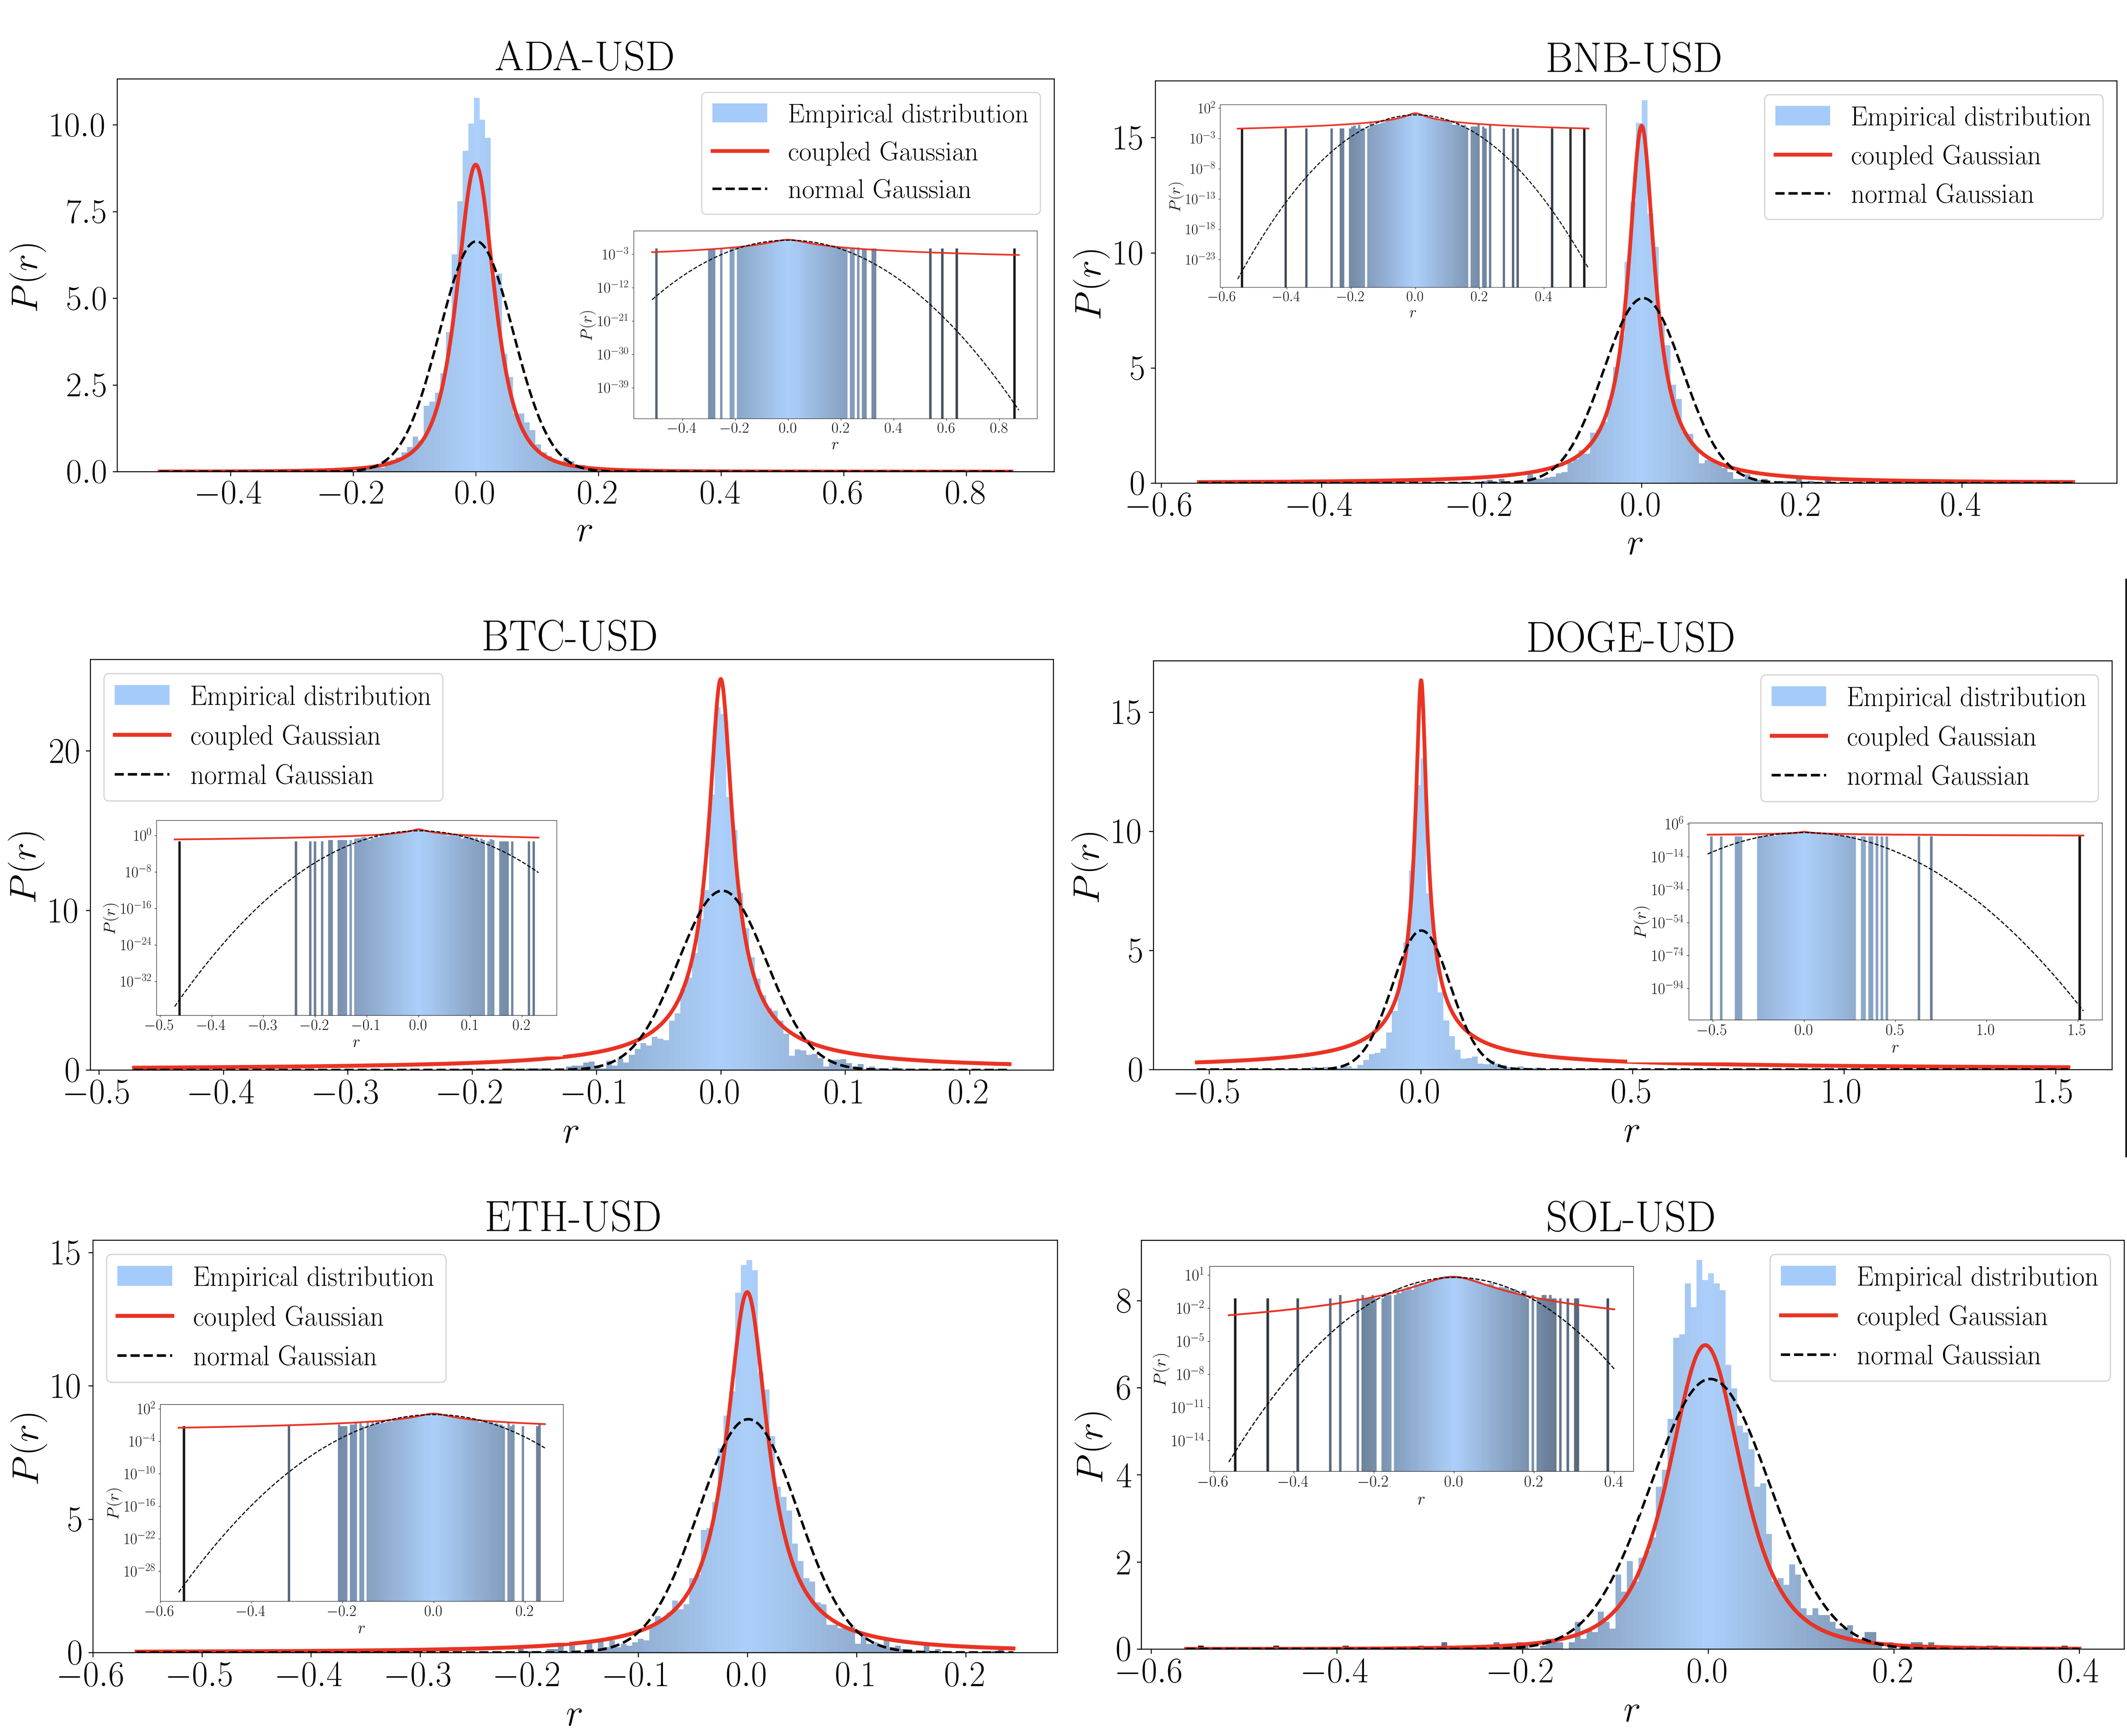
\includegraphics[width= \linewidth]{Fig_Crypto_Distro_Combined.png} 
		\begin{center}
            \caption{\textcolor{red}{update}Comparison between the normal Gaussian and the Coupled Gaussian fits to the empirical distribution of 6 different cryptocurrencies log returns, including (a) ADA, (B) Binance coin, (c) Bitcoin, (d) Doge coin, (e) Ethereum and (f) Solana. The inset displays the mono-log plot, highlighting the heavy-tailed nature of the data, captured bu the Coupled Gaussian fit but underestimated by the standard Gaussian.} 
		\label{Fig_Crypto_Distributions.png}
		\end{center}
	\end{center}
\end{figure}

Heavy tails break classical moment estimators.

\begin{itemize}
  \item \textbf{Independent Equals:} Draw samples from a modified distribution guaranteed to have finite variance while keeping functional tie to the original distribution.
  \item \textbf{Independent Approximates:} Samples with $q = \{2, 3\}$ yield pairs or triplets that are approximately equivalent.
\end{itemize}

Finite-variance estimation for machine learning;  Tractable training of complex systems.

\begin{figure}[ht!]
	\begin{center}
		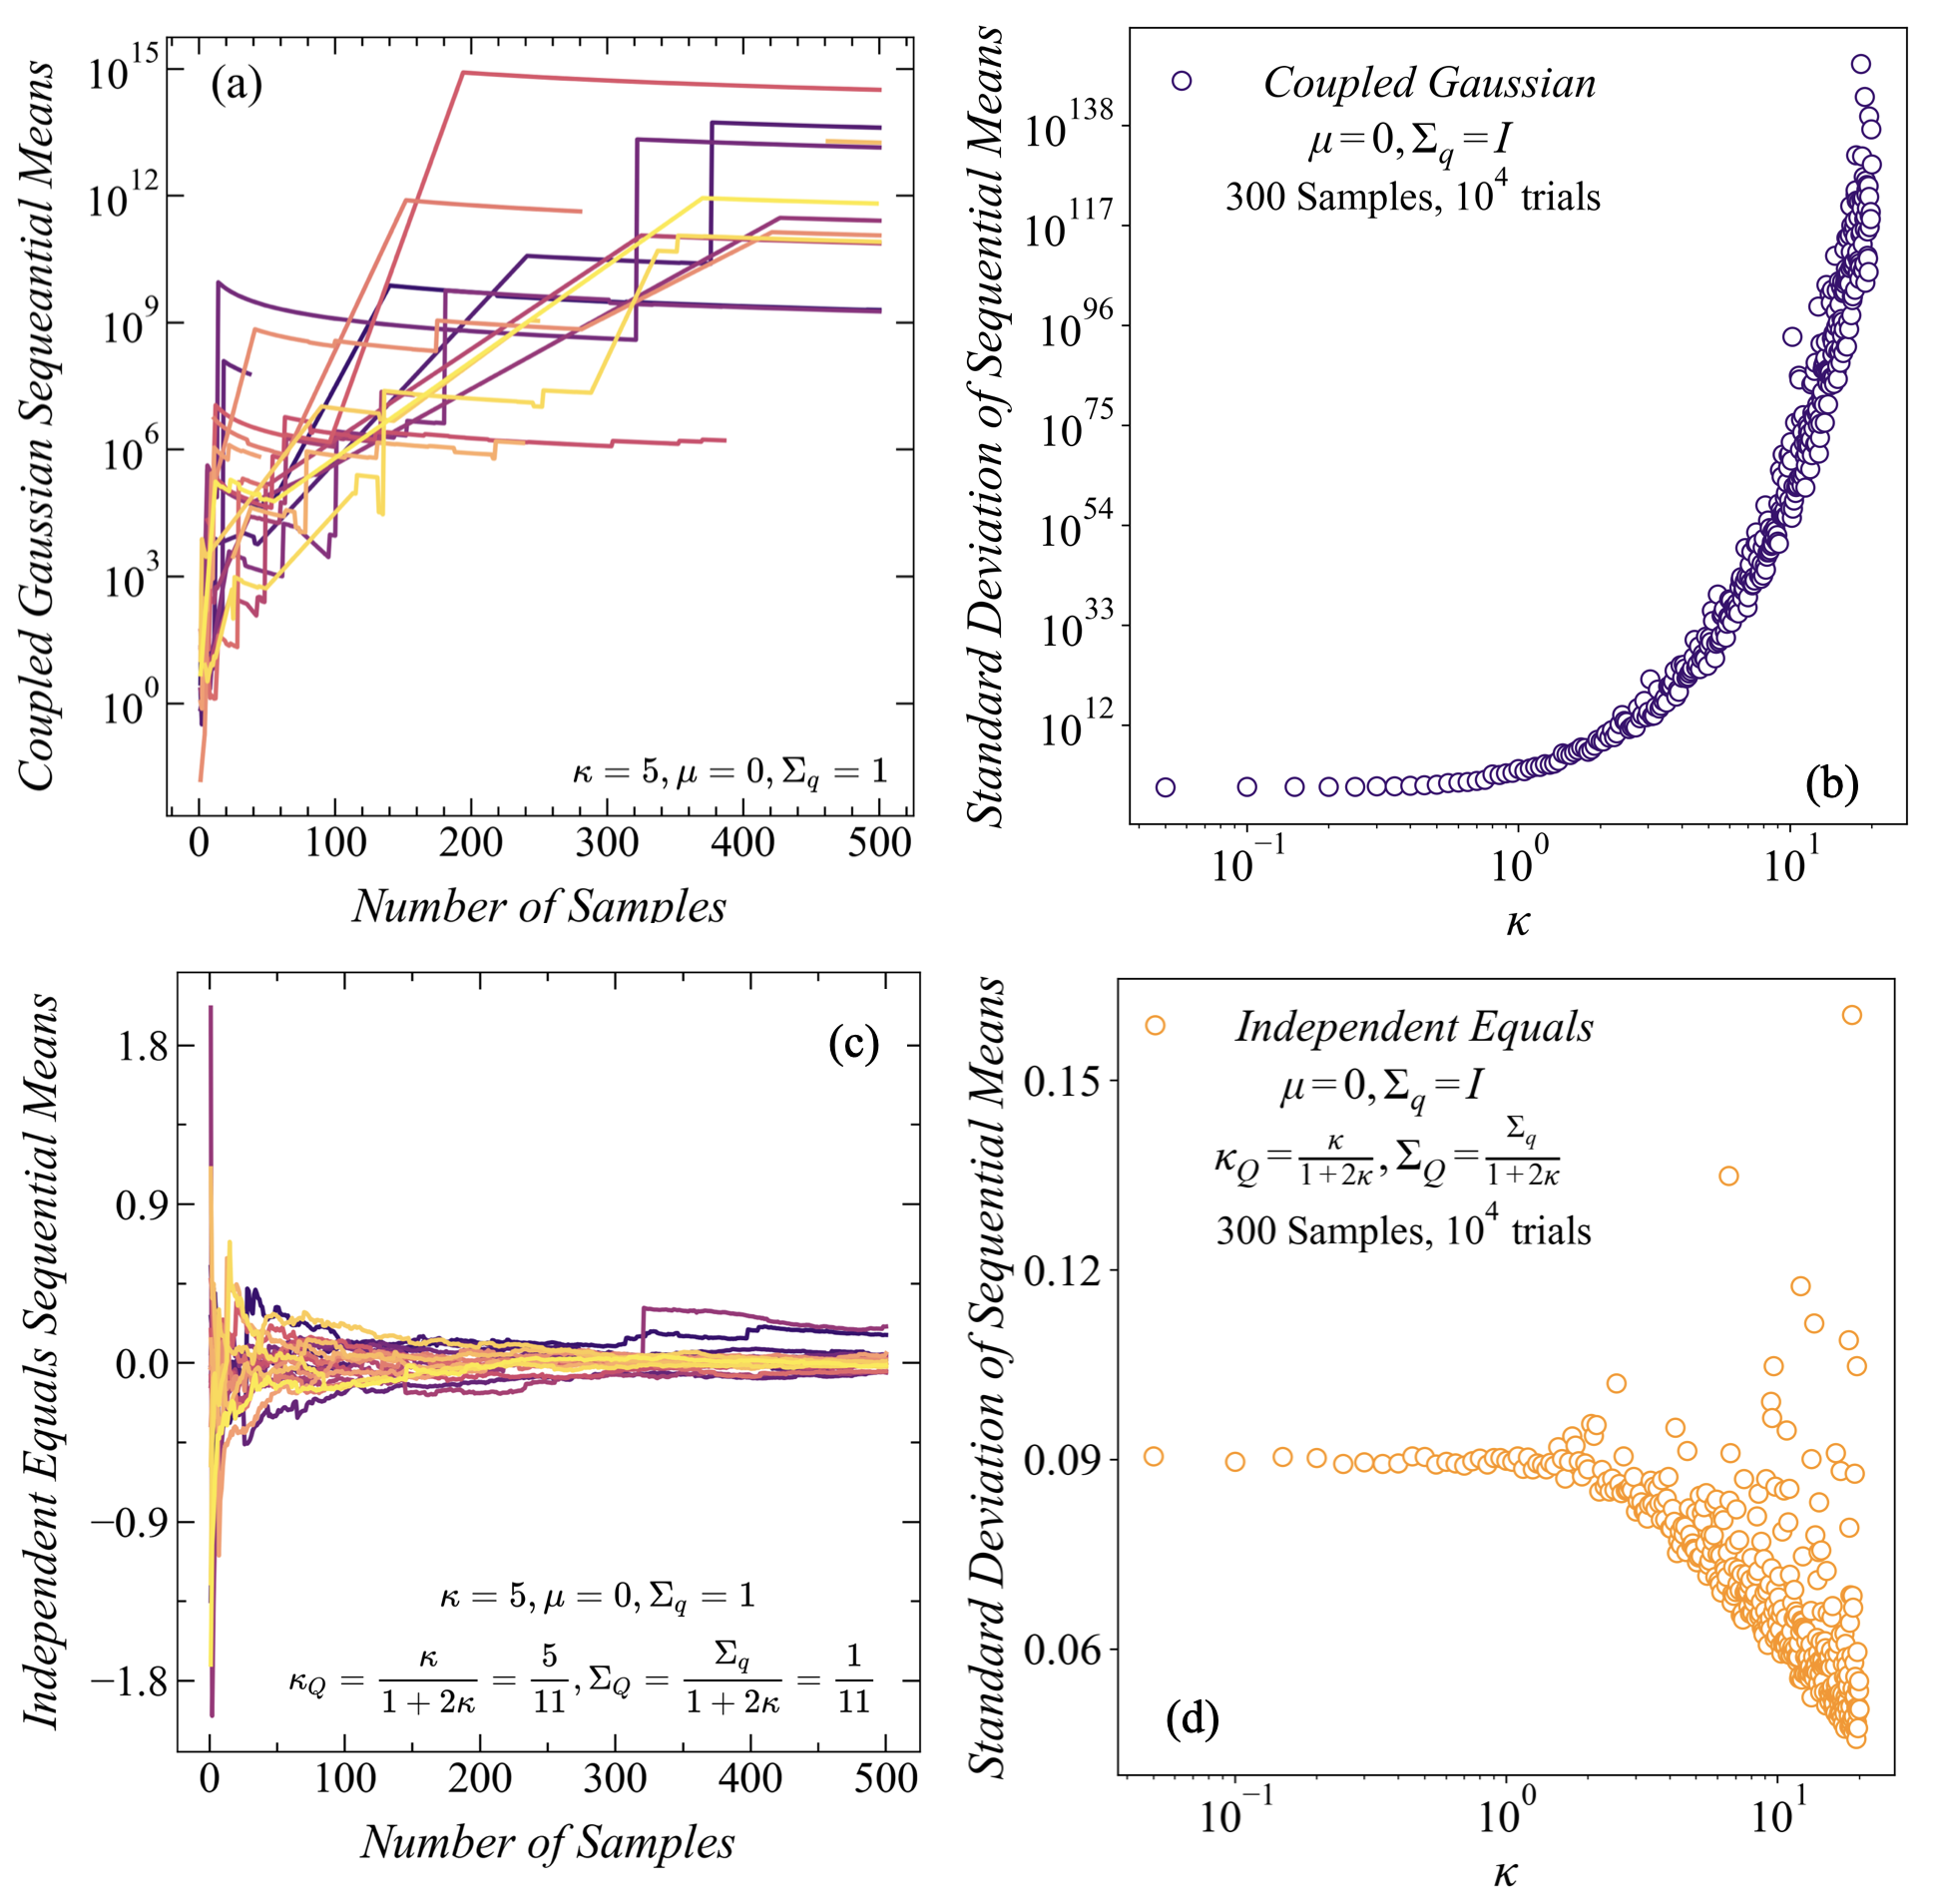
\includegraphics[width= \linewidth]{Fig_Sequential_means.png} 
		\begin{center}
            \caption{\textcolor{red}{update image quality! dimension?? update sigma! after the introduction of the independent-equals!  (d) vertical axis should go from zero to 0.25. Independent equals word color in orange!!}  (a) Coupled Gaussians are generated with Generalized Box–Muller ($\ln \rightarrow \ln$) and (b) have undefined sequential means for $\kappa > 1$. (c) Independent equals sequential means converge even for $\kappa > 1$, (d) yielding robust and finite-variance estimators.}
		\label{Fig_Sequential_means.png}
		\end{center}
	\end{center}
\end{figure}

\subsection{Learned Latent Space}

A comprehensive analysis of the learned latent space is crucial for understanding how the Coupled Variational Autoencoder (CVAE) organizes and disentangles the salient features of the input data. The CelebA dataset contains rich annotations providing $40$ binary attributes per image. These attributes span a wide range of facial characteristics, including demographic properties such as 'Male' and 'Young', aesthetic features like 'Smiling' and 'Bald', and accessory presence such as 'Eyeglasses' or 'Hat'. This extensive categorization allows for a granular examination of the model's internal representations.

Our initial approach to understanding the latent space structure involves extracting the mean ($\mu$) vectors from the encoded latent distributions for a substantial subset of the test data. Given that the latent dimensionality, $d$, can often exceed two, Principal Component Analysis (PCA) is employed as a linear dimensionality reduction technique to project these high-dimensional latent vectors into a two-dimensional plane. This 2D projection serves as the basis for scatter plots, where each point represents an image's latent representation, and these points are color-coded according to specific CelebA attributes, such as 'Male' or 'Smiling'. This visualization method reveals the degree to which the CVAE disentangles and distinguishes prominent features, enabling the assessment of clustering tendencies and the separation of attribute-specific groups. 









\textcolor{red}{do mnist neighbor latent space graph! calculate clustering and clustering to celeba??}

\textcolor{red}{old results below}
We present results on ensemble reconstruction for classic data sets including MNIST and CIFAR10 with original images and with corrupted images. 

We present original and reconstructed images for a visual confirmation of the generative process. Further insight is gained by the results of t-SNE plots, histogram analysis, and SSIM. 

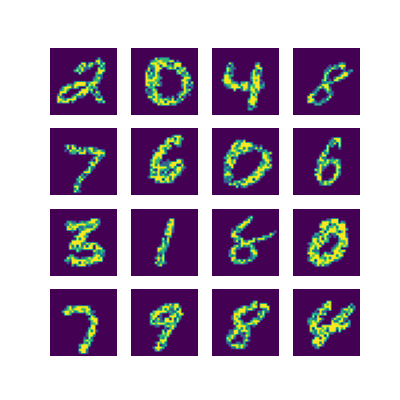
\includegraphics[scale=0.5]{original_images_cdX_clX_epoch}


\subsection{MNIST Shot Noise $\kappa=0$}

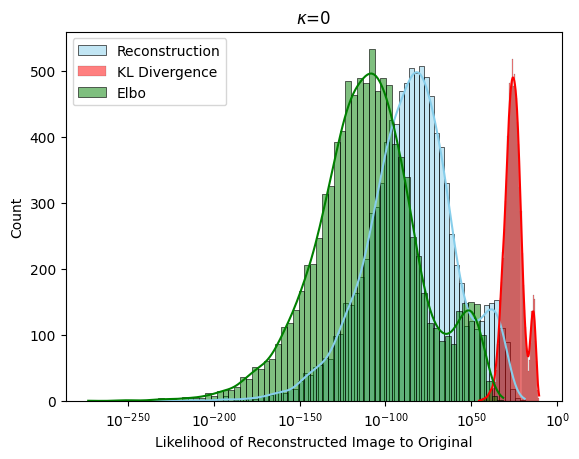
\includegraphics[scale=0.5]{kappa=0 beta=1}
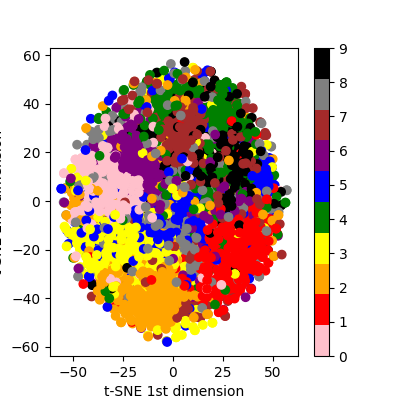
\includegraphics[scale=0.5]{latent_cdX_clX_epoch}
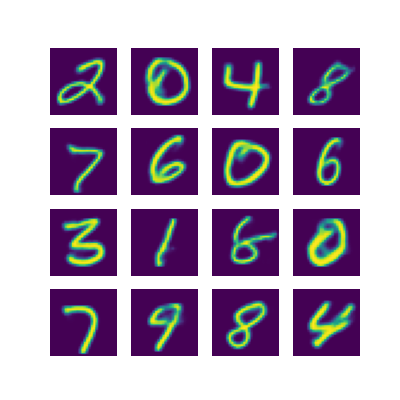
\includegraphics[scale=0.5]{images_cdX_clX_epoch}


\subsection{MNIST Shot Noise $\kappa=.1$}

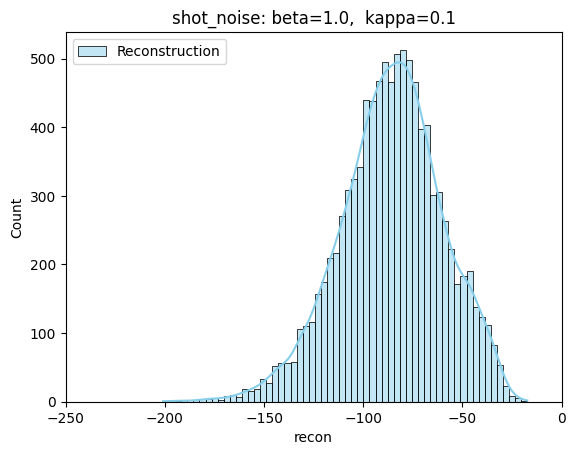
\includegraphics[scale=0.5]{images/hist beta=1 kappa=.1.png }
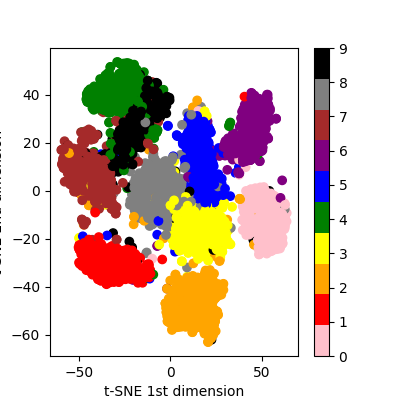
\includegraphics[scale=0.5]{images/latent_cdX_clX_epoch beta=1 kappa=.1.png}
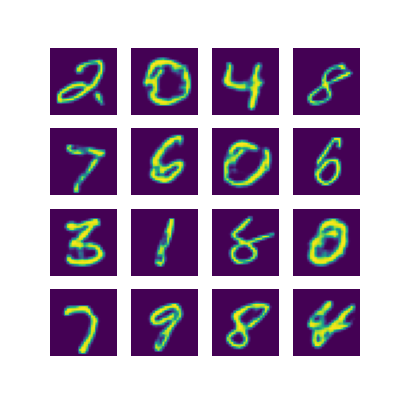
\includegraphics[scale=0.5]{images/images_cdX_clX_epoch beta=1 kappa=.1.png}



\section{Conclusion}

We have demonstrated an original capability to learn extreme models in which the slow decay of the asymptotic decay is far beyond any finite moments. The experimental results were conducted with a Coupled Variational Autoencoder architecture in which the latent distribution is a coupled Gaussian or Student's t distribution with the nonlinear statistical coupling much greater than one. The capability is enabled by the coupled free energy (or coupled negative evidence lower bound) cost function which leverages the unique properties of the coupled entropy. The coupled entropy combines a generalized logarithm metric with an expectation over the independent-equals modification to the measured distribution. For positive values of the nonlinear statistical coupling $(\kappa)$ this increases the cost of low-probability events while sampling from a distribution with fewer low-probability samples. The combination enables learning robust models with robust training statistics. Following a thorough literature search, it is the authors understanding that this capability has not been previously reported, given the conflicting requirements for robust models and robust statistics.

\section*{Acknowledgements}
Research on the Coupled Variational Autoencoder conducted between 2020 and 2023 provided valuable insights, although the results, which did not utilize the independent-equals distribution, were not published. We thank those investigators, Kevin Chen, Daniel Svoboda, John Clements, Hong Xiang Yue, and William Thistleton for their contributions.

\section*{Appendices}
\appendix

\section[First-order equivalence between the beta-VAE model and prior variance as a hyperparameter]
{First-order equivalence between the $\boldsymbol{\beta}$-VAE model and the prior variance as a hyperparameter}

In this appendix, we establish that, under a small-deviation regime, the effect of the $\beta$ coefficient in the $\beta$-VAE objective can be equivalently interpreted as a rescaling of the prior variance. We consider the one-dimensional case; the multivariate diagonal case follows by separability. Since $\beta$ is a multiplicative factor on the Kullback-Leibler divergence between the latent posterior and prior distributions, we focus on that portion of the ELBO. In this analysis the coupling is zero.

\begin{lemma}[First-order equivalence between $\beta$-VAE and prior variance]
\label{lemma:beta_prior_equivalence}
Let the prior and posterior latent variable be distributed as Gaussians:
\[
p(z) = \mathcal{N}(z;\mu_p,\sigma_p^2), 
\qquad
q(z|x) = \mathcal{N}(z;\mu_q,\sigma_q^2).
\]
Consider the $\beta$-weighted Kullback–Leibler divergence, $\beta D(q_\beta\|p_\beta)$, with unit prior variance, and the standard Kullback–Leibler divergence, $D(q\|p)$ with an arbitrary prior variance. Assume that the posterior is close to the prior in the sense that
\[
(\mu_q-\mu_p)^2 \approx 0,
\qquad
\sigma_q^2 = \sigma_p^2 + \epsilon,
\qquad
\sigma_{q,\beta}^2 = 1 + \epsilon_\beta,
\]
with $|\epsilon| \ll 1$ and $|\epsilon_\beta| \ll 1$. Then, to leading nontrivial order, the equivalence
\[
\beta D(q_\beta\|p_\beta) = D(q\|p)
\]
implies
\begin{equation}
\sigma_p^2 \approx \frac{1}{\sqrt{\beta}}.
\label{eq:beta_prior_equivalence_final}
\end{equation}
\end{lemma}

\begin{proof}
The Kullback–Leibler divergence between two univariate Gaussians is given by
\begin{equation}
\label{eq:kl_general_proof}
D_{\mathrm{KL}}(q\|p)
=
\frac{1}{2}
\left(
-\log \frac{\sigma_q^2}{\sigma_p^2}
+
\frac{\sigma_q^2}{\sigma_p^2}
+
\frac{(\mu_q-\mu_p)^2}{\sigma_p^2}
-1
\right).
\end{equation}

For a $\beta$-VAE with unit prior variance $\sigma_p^2 = 1$, the weighted divergence is
\begin{equation}
\label{eq:kl_beta_proof}
\beta D(q_\beta\|p_\beta)
=
\frac{\beta}{2}
\left(
-\log \sigma_{q,\beta}^2
+
\sigma_{q,\beta}^2
+
(\mu_{q,\beta}-\mu_{p,\beta})^2
-1
\right).
\end{equation}

We impose the matching condition
\begin{equation}
\beta D(q_\beta\|p_\beta) = D(q\|p).
\label{eq:matching_proof}
\end{equation}

In the regime where the posterior is close to the prior, we neglect mean discrepancies,
\[
(\mu_q-\mu_p)^2 \approx 0,
\qquad
(\mu_{q,\beta}-\mu_{p,\beta})^2 \approx 0,
\]
and parameterize the variance deviations as
\[
\sigma_q^2 = \sigma_p^2 + \epsilon,
\qquad
\sigma_{q,\beta}^2 = 1 + \epsilon_\beta,
\]
with $|\epsilon| \ll 1$ and $|\epsilon_\beta| \ll 1$.

Substituting into \eqref{eq:matching_proof}, we obtain
\begin{equation}
\beta\left[
\epsilon_\beta - \log(1+\epsilon_\beta)
\right]
=
\left[
\frac{\epsilon}{\sigma_p^2}
-
\log\left(1+\frac{\epsilon}{\sigma_p^2}\right)
\right].
\label{eq:reduced_proof}
\end{equation}

Using the Taylor expansion
\[
\log(1+x) = x - \frac{x^2}{2} + \mathcal{O}(x^3),
\]
we expand both sides of \eqref{eq:reduced_proof} up to second order:
\begin{align*}
\epsilon_\beta - \log(1+\epsilon_\beta)
&= \frac{\epsilon_\beta^2}{2} + \mathcal{O}(\epsilon_\beta^3), \\
\frac{\epsilon}{\sigma_p^2} - \log\left(1+\frac{\epsilon}{\sigma_p^2}\right)
&= \frac{\epsilon^2}{2\sigma_p^4} + \mathcal{O}(\epsilon^3).
\end{align*}

Substituting these expansions into \eqref{eq:reduced_proof}, we obtain
\[
\beta \cdot \frac{\epsilon_\beta^2}{2}
=
\frac{\epsilon^2}{2\sigma_p^4}.
\]

Solving for $\sigma_p^2$ yields
\begin{equation}
\sigma_p^2
=
\frac{\epsilon}{\epsilon_\beta}\cdot \frac{1}{\sqrt{\beta}}.
\end{equation}

Assuming that the deviations $\epsilon$ and $\epsilon_\beta$ are of the same order, i.e.,
\[
\frac{\epsilon}{\epsilon_\beta} \approx 1,
\]
we obtain the leading-order relation
\[
\sigma_p^2 \approx \frac{1}{\sqrt{\beta}}.
\]

This establishes the first-order equivalence between the $\beta$ coefficient and the prior variance.
\end{proof}

The result extends component-wise to diagonal multivariate Gaussians. In the case of full covariance matrices, the equivalence corresponds to an isotropic rescaling $\mathbf{\Sigma}_p \mapsto \mathbf{\Sigma}_p / \sqrt{\beta}$ under the same small-deviation assumptions.

That result shows that the beta-VAE performance can be obtained with a standard VAE with prior variance $    \sigma_p^2 = \frac{1}{\sqrt{\beta}}$. Therefore, the effects of adding the hyperparameter $\beta$ can be obtained just by tuning the prior variance.



\section{Proof of the Coupled Free Energy}

In this appendix, we derive the closed-form expression of the Coupled Free Energy (CFE) for multivariate coupled Gaussian distributions. Both the latent distribution and noise model for the data have coupled Gaussian distributions with nonlinear statistical coupling $\kappa \geq 0.$

In this context, we define $R(\kappa,\alpha=2,d):=\frac{\kappa}{1+\kappa d/2}.$
We interpret $R(\kappa,2,d)$ as the informational relative risk aversion, given its role in modifying the cost of information. This quantity provides a compact measure of the joint influence of tail heaviness $\kappa$, the stretching parameter, which equals 2 for the Gaussian, and the dimension $d$. The extensivity of the coupled entropy, measured by the Hanel-Thurner long-range scaling parameter \citep{hanelComprehensiveClassificationComplex2011,nelsonUniqueUniversalEntropy2026}, is equal to $R(\kappa,2,d)/2$.

\begin{lemma}\label{Normalization} \textbf{Normalization of the independent-equals coupled Gaussian.} Let
\[
q(z \mid x) = \frac{1}{Z(\mathbf{\Sigma}_q, \kappa,\alpha)}
\Bigl(1 + \kappa \bigl[\tfrac{1}{2}(z-\mu_q)^{\!\intercal} \mathbf{\Sigma}_q^{-1} (z-\mu_q)\bigr]\Bigr)^{-\frac{1 + \kappa d/2}{\kappa}}, 
\]
be a $d$-dimensional multivariate coupled Gaussian with stretching parameter ($\alpha=2$), mean $(\mu_q \in \mathbb{R}^d)$, positive-definite scale matrix $(\mathbf{\Sigma}_q \in \mathbb{R}^{d \times d})$, and nonlinear statistical coupling parameter ($\kappa > 0$).
Define  
\[
q/^{\iota(\kappa,d_2)}(z \mid x) \;:=\; \frac{q(z \mid x)^{1 + \frac{\kappa}{1+\kappa d/2}}}
{\int_{\mathbb{R}^d} q(z \mid x)^{1 + \frac{\kappa}{1+\kappa d/2}} \, dz}.
\]
Then $(q/^{\iota(\kappa,d_2)}(z \mid x))$ is the independent-equals distribution, which is a multivariate coupled Gaussian, with the same mean $(\tilde\mu_q = \mu_q)$ and modified coupling and scale parameters,  
\[
\tilde\kappa= \frac{\kappa}{1+\kappa}, \ 
\widetilde{\mathbf{\Sigma}}_q =  \frac{\mathbf{\Sigma}_q}{1+\kappa}.
\]
Explicitly,  the independent-equals distribution is
\[
q/^{\iota(\kappa,d_2)}(z \mid x) = \frac{1}{\widetilde Z_q(\mathbf{\widetilde\Sigma}_q, \tilde\kappa,2)}
\Bigl(1 + \tilde\kappa \bigl[\tfrac{1}{2}(z-\tilde\mu_q)^{\!\intercal} \mathbf{\widetilde\Sigma}_q^{-1} (z-\tilde\mu_q)\bigr]\Bigr)^{-\frac{1 + \tilde\kappa d/2}{\tilde\kappa}},
\]
where the normalization constant is given by 
\begin{align}
    \widetilde Z_q(\mathbf{\widetilde\Sigma_q}, \tilde\kappa)  
    &=\pi^\frac{d}{2}
|\boldsymbol{\widetilde\Sigma}_q|^\frac{1}{2}
\left\{
\begin{matrix}
    \left(\frac{\tilde{\kappa}}{2}\right)^{-d/2}
    \frac{\Gamma(\frac{1}{\tilde{\kappa}})}{\Gamma(\frac{d}{2}+\frac{1}{\tilde{\kappa}})}
    & \tilde\kappa > 0 \\
    2^{d/2} & \tilde\kappa=0.
\end{matrix}
\right.
\end{align}
\end{lemma}

\begin{proof} 
To construct the independent-equals 
$q/^{\iota(\kappa,d_2)}(z \mid x)$, 
we start by raising $(q(z \mid x))$ to the power
\[
1 + \frac{\kappa}{1+\kappa d/2}
=\frac{1+\kappa(d/2+1)}{1+\kappa d/2},
\]
obtaining
\begin{equation}\label{coupledGaussianPowerBeta}
q/^{\iota(\kappa,d_2)}(z \mid x) \propto
\Bigl(1 + \kappa 
\bigl[\tfrac{1}{2}(z-\mu_q)^{\!\intercal} 
\mathbf{\Sigma}_q^{-1} (z-\mu_q)
\bigr]
\Bigr)^{-\frac{1+\kappa(d/2+1)}{\kappa}}.
\end{equation}

The normalization constant of this power density is  
\begin{equation}\label{Zq1}
\tilde Z_q := \int_{\mathbb{R}^d}\Bigl(
1 + \kappa \bigl[\tfrac{1}{2}(z-\mu_q)^{\!\intercal} 
\mathbf{\Sigma}_q^{-1} (z-\mu_q)\bigr]
\Bigr)^{-\frac{1+\kappa(d/2+1)}{\kappa}}\, dz.
\end{equation}

To compute the partition function $\tilde Z_q$, we set 
$y = z - \mu_q$ and diagonalize the scale matrix by writing
$\mathbf{\Sigma}_q^{-1} = U \Lambda^{-1} U^{\!\intercal}$ 
where $U$ is orthogonal and 
$\Lambda = \operatorname{diag}(\lambda_1,\dots,\lambda_d)$ 
is a diagonal matrix. Hence, considering the rotation transformation 
$s = U^{\!\intercal} y$ with unitary Jacobian, we calculate
\begin{equation}\label{diagonalization}
y^{\!\intercal} \mathbf{\Sigma}_q^{-1} y
=(U^{\!\intercal}y)^{\!\intercal} 
\Lambda^{-1} (U^{\!\intercal}y)
=\sum_{i=1}^d \frac{s_i^2}{\lambda_i}.
\end{equation}

Thus, substituting Eq.~\eqref{diagonalization} into Eq.~\eqref{Zq1}, we write the normalization constant as
\begin{equation}\label{Zq2}
\tilde Z_q=\int_{\mathbb{R}^d}\Bigl(
1 + \frac{\kappa}{2}\sum_{i=1}^d \frac{s_i^2}{\lambda_i}\Bigr)^{-\gamma}\, ds,\qquad
\gamma \equiv \frac{1+\kappa(d/2+1)}{\kappa}.
\end{equation}

Now, recall that by taking the Gamma-integral
\[
\Gamma(\gamma)
=
\int_0^\infty \tau^{\gamma-1} e^{-\tau} d\tau
\]
and by doing the change of variables 
$\tau=t(1+u)$, we obtain the identity
\begin{equation}\label{GammaIdentity}
(1+u)^{-\gamma}=\frac{1}{\Gamma(\gamma)}
\int_0^\infty t^{\gamma-1} e^{-t(1+u)}\, dt.
\end{equation}

Thus, applying Eq.~\eqref{GammaIdentity} into Eq.~\eqref{Zq2} with
\[
u = \frac{\kappa}{2}\sum_{i=1}^d \frac{s_i^2}{\lambda_i},
\]
we obtain
\begin{equation}\label{Zq3}
\tilde Z_q
=\frac{1}{\Gamma(\gamma)}\int_0^\infty
t^{\gamma-1} e^{-t}\Bigl[\int_{\mathbb{R}^d}
\exp\!\Bigl(-t\frac{\kappa}{2}
\sum_{i=1}^d \frac{s_i^2}{\lambda_i}\Bigr)\, ds
\Bigr]dt.
\end{equation}

The inner integral factorizes as a product of Gaussian integrals:
\begin{equation}\label{GaussianIntegral}
\begin{aligned}
\int_{\mathbb{R}^d}\exp\!\Bigl(-t\frac{\kappa}{2}
\sum_{i=1}^d \frac{s_i^2}{\lambda_i}
\Bigr)ds
&=
\prod_{i=1}^d\int\exp\!\Bigl(-t\frac{\kappa}{2}
\frac{s_i^2}{\lambda_i}\Bigr)ds\\
&=
\prod_{i=1}^d\sqrt{\frac{2\pi\lambda_i}{t\kappa}
}\\
&=
\Bigl(\frac{2\pi}{t\kappa}\Bigr)^{d/2}
\sqrt{|\mathbf{\Sigma}_q|}.
\end{aligned}
\end{equation}

Substituting back Eq.~\eqref{GaussianIntegral} into Eq.~\eqref{Zq3} yields
\[
\tilde Z_q
=\frac{\sqrt{|\mathbf{\Sigma}_q|}}
{\Gamma(\gamma)}\Bigl(\frac{2\pi}{\kappa}
\Bigr)^{d/2}\int_0^\infty
t^{\gamma-1-d/2}e^{-t}\, dt.
\]

Note that the remaining integral is simply
\[
\Gamma(\gamma-d/2),
\]
where
\[
\gamma-\frac{d}{2}
=\frac{1+\kappa(d/2+1)}{\kappa}-\frac{d}{2}
=\frac{1+\kappa}{\kappa}.
\]

Hence, we obtain the normalization constant of the independent-equals distribution:
\begin{equation}\label{Q_partition_function}
\tilde Z_q
=
\frac{
\Gamma\!\Bigl(\frac{1+\kappa}{\kappa}\Bigr)
}{
\Gamma\!\Bigl(\frac{1+\kappa(d/2+1)}{\kappa}\Bigr)
}
\sqrt{\Bigl(\frac{2\pi}{\kappa}\Bigr)^d|\mathbf{\Sigma}_q|
}.
\end{equation}

Now, writing the independent-equals distribution in the standard coupled-Gaussian form
\begin{equation}\label{Q_standard_Equation}
q/^{\iota(\kappa,d_2)}(z \mid x)
=
\frac{1}{\widetilde Z_q}
\Bigl(1+\tilde{\kappa}\bigl[\tfrac12 y^\top
\widetilde{\mathbf{\Sigma}}_q^{-1}y\bigr]
\Bigr)^{-\frac{1+\tilde{\kappa} d/2}{\tilde{\kappa}}},\qquad y=z-\mu_q,
\end{equation}
and combining with Eq.~\eqref{coupledGaussianPowerBeta} and comparing the exponents, we obtain
\begin{equation}\label{kappa}
\frac{1+\tilde{\kappa} d/2}{\tilde{\kappa}}
=
\frac{1+\kappa(d/2+1)}{\kappa}
\quad\Longrightarrow\quad
\tilde{\kappa}
=
\frac{\kappa}{1+\kappa}.
\end{equation}

In addition to that, by combining
Eqs.~\eqref{Q_standard_Equation}
and \eqref{coupledGaussianPowerBeta},
the equality of the quadratic forms for all $y$ requires that the scale matrices satisfy
\[
\kappa\bigl[\tfrac12y^{\!\intercal}\mathbf{\Sigma}_q^{-1}y\bigr]=
\tilde{\kappa}\bigl[\tfrac12y^{\!\intercal}
\widetilde{\mathbf{\Sigma}}_q^{-1}y\bigr]
\qquad \forall y.
\]

Thus, it follows that
\[
\kappa\,\mathbf{\Sigma}_q^{-1}
=
\tilde{\kappa}\,\widetilde{\mathbf{\Sigma}}_q^{-1}.
\]

Substituting back Eq.~\eqref{kappa}, we get
\begin{equation}
\widetilde{\mathbf{\Sigma}}_q
=
\frac{\mathbf{\Sigma}_q}{1+\kappa}.
\end{equation}

Therefore, combining the above results, the independent-equals density preserves the coupled-Gaussian form with parameters
\[
\tilde{\kappa}=\frac{\kappa}{1+\kappa},
\qquad
\widetilde{\mathbf{\Sigma}}_q
=
\frac{\mathbf{\Sigma}_q}{1+\kappa}.
\]
\end{proof}


\begin{lemma}[Second independent-equals moment of a coupled Gaussian]\label{second_moment}
Given a $d$-dimensional multivariate coupled Gaussian with mean $(\mu_q \in \mathbb{R}^d)$, positive-definite scale matrix $(\mathbf{\Sigma}_q \in \mathbb{R}^{d \times d})$, and nonlinear statistical coupling $(\kappa>0)$
\begin{equation}
Z|(X=x) \sim q(z \mid x) = \frac{1}{Z(\mathbf{\Sigma}_q, \kappa)}
\Bigl(1 + \kappa \bigl[\tfrac{1}{2}(z-\mu_q)^{\!\intercal} \mathbf{\Sigma}_q^{-1} (z-\mu_q)\bigr]\Bigr)^{-\frac{1 + \kappa d/2}{\kappa}}, 
\end{equation}
such that
\[
1 + \kappa \bigl[\tfrac{1}{2}(z-\mu_q)^{\!\intercal} \mathbf{\Sigma}_q^{-1} (z-\mu_q)\bigr] >0.
\]
with independent-equals distribution 
\begin{equation}
q/^{\iota(\kappa,d_2)}(z \mid x)
\;:=\;\frac{
q(z \mid x)^{1 + \frac{\kappa}{1+\kappa d/2}}
}{\int_{\mathbb{R}^d}
q(z \mid x)^{1 + \frac{\kappa}{1+\kappa d/2}}
\, dz},
\end{equation}
with mean $\tilde{\mu}_q = \mu_q \in \mathbb{R}^d$, positive definite scale matrix $\widetilde{\mathbf{\Sigma}}_q \in \mathbb{R}^{d \times d}$ and nonlinear statistical coupling
\[
\tilde{\kappa} = \frac{\kappa}{1+\kappa}.
\]
Define the centered variable $y_q= z - \mu_q$. Then,
\[
\mathbb{E}_{q/^{\iota(\kappa,d_2)}(\textbf{z}\mid \textbf{x})}
\!\left[y_q y_q^\intercal\right]
=\Sigma_q,
\]
and consequently,
\[
\mathbb{E}_{q/^{\iota(\kappa,d_2)}(\textbf{z}\mid \textbf{x})}
\!\left[y_q^\intercal \Sigma_q^{-1} y_q\right]=d.
\]
\end{lemma}

\begin{proof}
The coupled Gaussian density of the centered variable $y_q = z-\mu_q$ is
\[
q/^{\iota(\kappa,d_2)}(\textbf{z}\mid \textbf{x})
=
Z_q^{-1}
\left(
1 + \kappa\, \Bigl[\tfrac{1}{2}y_q^\intercal \Sigma_q^{-1} y_q\Bigr]
\right)^{-\gamma_1},
\quad
\gamma_1 \equiv \frac{1+\kappa(d+2)/2}{\kappa},
\]
where $Z_q = \tilde{Z}_q$ denotes the normalization constant as calculated in Lemma \ref{Normalization}, given by Eq.\eqref{Q_partition_function}, and $\kappa=\tilde{\kappa}$. Using the identity $a^\intercal M a = \operatorname{Tr}(M a a^\intercal)$,
we calculate the expectation over the independent-equals distribution as
\begin{equation} \label{1th_stamente,lemma2}
    \mathbb{E}_{q/^{\iota(\kappa,d_2)}(\textbf{z}\mid \textbf{x})}\!\left[y_q^\intercal \Sigma_q^{-1} y_q\right]
=
\operatorname{Tr}
\!\left(
\Sigma_q^{-1}\mathbb{E}_{q/^{\iota(\kappa,d_2)}(\textbf{z}\mid \textbf{x})}[y_q y_q^\intercal]
\right),    
\end{equation}
where 
\begin{align}\label{exp}
\mathbb{E}_{q/^{\iota(\kappa,d_2)}(\textbf{z}\mid \textbf{x})}\left[y_qy_q^{\intercal}\right]
=
\frac{1}{Z_q}
\int
\left(y_q y_q^{\intercal}\right)
\left(
1+\kappa\, \Bigl[\tfrac{1}{2}y_q^{\intercal}\Sigma_q^{-1}y_q\Bigr]
\right)^{-\gamma_1}
\,dy_q,
\end{align}
is the second-order moment. To compute Eq. \eqref{exp}, we consider the eigen-decomposition of the scale matrix:
\[
\Sigma_q^{-1} = U_q \Lambda_q^{-1} U_q^\intercal,
\]
where $U_q$ is an orthogonal matrix and $\Lambda_q=\mathrm{diag}(\lambda_{q_1},\dots,\lambda_{q_d})$ is a diagonal matrix. Applying the eigen-decomposition transformation to Eq.\eqref{exp}, we obtain
\begin{align} \label{exp2}
\mathbb{E}\left[y_qy_q^{\intercal}\right]=\frac{1}{Z_q}\int\left(y_q y^\intercal_q\right)\left(1+\kappa\Bigl[\tfrac{1}{2}\left( y_q^{\intercal}U_q\Lambda_q^{-1}U_q^{\intercal}y_q\right)\Bigr]\right)^{-\gamma_1} dy_q.
\end{align}
We define the rotated variable $s_q = U_q^\intercal y_q$, %with $ds_q=U_q^\intercal dy_q$. Since $U_q$ is orthogonal, 
the Jacobian of the transformation is equal to one, implying $ds_q = dy_q$. Under this change of variables, the quadratic form diagonalizes:
\begin{equation} \label{diag}
    y_q^\intercal \Sigma_q^{-1} y_q= (U_q^\intercal y_q)^\intercal
\Lambda_q^{-1}(U_q^\intercal y_q) =  s_q^\intercal \Lambda_q^{-1} s_q =\sum_{r=1}^d \frac{s_{q_r}^2}{\lambda_{q_r}}.
\end{equation}
Applying Eq. \eqref{diag} in the Eq. \ref{exp2}, and noting that $y_q = U_q s_q$, we obtain
\begin{equation}
    \begin{split}
        \mathbb{E}_{q/^{1+ \frac{\kappa}{1+\kappa d/2}}(\textbf{z}\mid \textbf{x})}[y_q y_q^\intercal]
& =\frac{1}{Z_q}\int\left(U_qs_qs_q^\intercal U_q^\intercal\right)
\left(1 + \kappa \Bigl[\tfrac{1}{2}\sum_{r=1}^d \frac{s_{q_r}^2}{\lambda_{q_r}}\Bigr]\right)^{-\gamma_1}ds_q \\ & =U_q\left[\frac{1}{Z_q}\int s_q s_q^\intercal
\left(1 + \kappa \Bigl[\tfrac{1}{2}\sum_{r=1}^d \frac{s_{q_r}^2}{\lambda_{q_r}}\Bigr]\right)^{-\gamma_1}ds_q\right]
U_q^\intercal. \label{exp3}
    \end{split}
\end{equation}
The brackets contains a matrix-valued integral which $(i,j)$-th entry is given by
\begin{equation}\label{matrixIntegral}
\int s_{q_i}s_{q_j}
\left(
1 + \kappa \Bigl[\tfrac{1}{2}\sum_{r=1}^d \frac{s_{q_r}^2}{\lambda_{q_r}}\Bigr]
\right)^{-\gamma_1}
ds_q.
\end{equation}
If $i \neq j$, the integrand of Eq. \eqref{matrixIntegral} is an odd function with respect to $s_{q_i}$ or $s_{q_j}$, while the integration domain is symmetric. Therefore, all off-diagonal terms vanish. However, for $i=j$, the integrand is even, and the integral has a non-zero value. To evaluate the diagonal terms, we use the 
Gamma-function representation
\begin{equation}\label{gammaRep}
    (1+u)^{-\gamma_1}
=
\frac{1}{\Gamma(\gamma_1)}
\int_0^\infty t^{\gamma_1-1} e^{-t(1+u)}dt.
\end{equation}
By applying Eq. \eqref{gammaRep} to Eq.\eqref{matrixIntegral} with $u = \kappa \Bigl[\tfrac{1}{2}\sum_{r=1}^d s_{q_r}^2/\lambda_{q_r}\Bigr]$ and $i=j$, we get
\begin{align}\label{Gama_fun}
\int s_{q_i}^2
\left(
1 + \kappa \Bigl[\tfrac{1}{2}\sum_{r=1}^d \frac{s_{q_r}^2}{\lambda_{q_r}}\Bigr]
\right)^{-\gamma_1}
ds_q
=
\frac{1}{\Gamma(\gamma_1)}
\int_0^\infty t^{\gamma_1-1} e^{-t}
\left[
\int s_{q_i}^2
\exp \left( -\tfrac{t\kappa}{2} \sum_{r=1}^d \frac{s_{q_r}^2}{\lambda_{q_r}} \right ) 
ds_q
\right]
dt.
\end{align}
Note that the inner integral inside the brackets factorizes into independent one-dimensional Gaussian integrals:
\begin{equation}
    \begin{split}
        \int s_{q_i}^2 \exp \left( -\tfrac{t\kappa}{2} \sum_{r=1}^d \frac{s_{q_r}^2}{\lambda_{q_r}} \right ) ds_q
& =
\left[ \prod_{\substack{r=1 \\ r \neq i}}^{d} 
 \int \exp \left( -\tfrac{t\kappa}{2} \frac{s_{q_r}^2}{\lambda_{q_r}} \right ) 
 ds_{q_r} \right]
\int s_{q_i}^2 \exp \left (-\tfrac{t \kappa}{2} \frac{s_{q_i}^2}{\lambda_{q_i}} \right ) ds_{q_i} \\&=  \left[ \prod_{\substack{r=1 \\ r \neq i}}^{d} \sqrt{\frac{2\pi \lambda_{q_r}}{t \kappa}}\right] \frac{\lambda_{q_i}}{t\kappa}  \sqrt{\frac{2\pi \lambda_{q_i}}{t \kappa}} =  \frac{\sqrt{(2\pi)^d|\Sigma_q|}}{(t\kappa)^{\frac{d+2}{2}}}
\lambda_{q_i}. \label{gausInts}
    \end{split}
\end{equation}
Thus, all diagonal elements coincide up to the corresponding eigenvalue,
and the resulting matrix is proportional to $\Lambda_q$. Hence, substituting Eq. \eqref{gausInts} into Eq. \eqref{Gama_fun} and integrating over $t$ yields
\begin{equation*}
    \int s_{q_i}^2
\left(
1 + \kappa \Bigl[\tfrac{1}{2}\sum_{r=1}^d \frac{s_{q_r}^2}{\lambda_{q_r}}\Bigr]
\right)^{-\alpha}
ds_q
= %\frac{1}{Z_q}
\frac{\sqrt{(2\pi)^d|\Sigma_q|}}{\kappa^{\frac{d+2}{2}}}
\frac{\Gamma\!\left(\gamma_1-\frac{d+2}{2}\right)}
{\Gamma(\gamma_1)}\lambda_{q_i}.
\end{equation*}
Therefore, the matrix-valued integral is 
\begin{equation} \label{matrixIntegral_1}
\int s_q s_q^\intercal
\left(1 + \kappa \Bigl[\tfrac{1}{2}\sum_{r=1}^d \frac{s_{q_r}^2}{\lambda_{q_r}}\Bigr]\right)^{-\gamma_1}ds_q
= %\frac{1}{Z_q}
\frac{\sqrt{(2\pi)^d|\Sigma_q|}}{\kappa^{\frac{d+2}{2}}}
\frac{\Gamma\!\left(\gamma_1-\frac{d+2}{2}\right)}
{\Gamma(\gamma_1)}\Lambda_q.
\end{equation}
Finally, substituting back Eq. \eqref{matrixIntegral_1} to Eq. \eqref{exp3}, we obtain
\begin{equation} 
\begin{split}
    \mathbb{E}_{q/^{1+ \frac{\kappa}{1+\kappa d/2}}(\textbf{z}\mid \textbf{x})}[y_q y_q^\intercal] & = U_q\left(\frac{1}{Z_q}\frac{\sqrt{(2\pi)^d|\Sigma_q|}}{\kappa^{\frac{d+2}{2}}}
\frac{\Gamma\!\left(\gamma_1-\frac{d+2}{2}\right)}
{\Gamma(\gamma_1)}\Lambda_q\right)U_q^\intercal\\
& =  \left(\frac{1}{Z_q}\frac{\sqrt{(2\pi)^d|\Sigma_q|}}{\kappa^{\frac{d+2}{2}}}
\frac{\Gamma\!\left(\gamma_1-\frac{d+2}{2}\right)}
{\Gamma(\gamma_1)}\right) U_q\Lambda_q U_q^\intercal\\
& =\frac{1}{Z_q}\frac{\sqrt{(2\pi)^d|\Sigma_q|}}{\kappa^{\frac{d+2}{2}}}
\frac{\Gamma\!\left(\gamma_1-\frac{d+2}{2}\right)}
{\Gamma(\gamma_1)} \Sigma_q \label{exp4}
\end{split}
\end{equation}
Now, substituting the normalization constant given by Eq. \eqref{Q_partition_function}
\[
Z_q
=
\frac{\Gamma\!\left(\frac{1}{\kappa}\right)}
{\Gamma(\gamma_1)}
\sqrt{\left(\frac{2\pi}{\kappa}\right)^d |\Sigma_q|},
\]
into Eq. \eqref{exp4} and using the identity $\Gamma(x+1)=x\Gamma(x)$ together with
\[
\gamma_1= \frac{1+\kappa(d+2)/2}{\kappa}
= \frac{1}{\kappa}+\frac{d}{2},
\]
yields the second moment expectation:
\begin{equation} \label{secondMomentEQ}
     \mathbb{E}_{q/^{1+ \frac{\kappa}{1+\kappa d/2}}(\textbf{z}\mid \textbf{x})}[y_q y_q^\intercal] = \Sigma_q,    
\end{equation}
preserving the second moment expectation of the original distribution. Finally, applying Eq.\eqref{secondMomentEQ} to Eq. \eqref{1th_stamente,lemma2}, we calculate 
\[
\mathbb{E}\!\left[
y_q^\intercal\Sigma_q^{-1}y_q
\right]
= \operatorname{tr}\!\left(
\Sigma_q^{-1}\mathbb{E}[y_q y_q^\intercal]
\right)
=
\operatorname{tr}(\Sigma_q^{-1}\Sigma_q)
=
\operatorname{tr}(I_d)
=
d.
\]
\end{proof}

\begin{theorem}[Coupled Free Energy for Multivariate Coupled Gaussian] \label{theorem_CFE}
Let $\boldsymbol{x} \in \mathbb{R}^d$ and $\mathbf{z} \in \mathbb{R}^d$ be random vectors, and suppose that the posterior $q_{\phi}(\mathbf{z} \mid \boldsymbol{x})$, the prior $p_{\theta}(\mathbf{z})$, and the data $p_\theta(x|z)$ are each multivariate coupled Gaussian with their joint PDFs defined as:
{\small
\begin{equation*}
f\left(\boldsymbol{x}; \boldsymbol{\mu}, \boldsymbol{\Sigma}, \kappa \right) \equiv 
\begin{cases}
\frac{1}{Z(\boldsymbol{\Sigma}, \kappa)}
\left(1 + \kappa \left[\frac{1}{2}(\boldsymbol{x} - \boldsymbol{\mu})^{\intercal}
\boldsymbol{\Sigma}^{-1} (\boldsymbol{x} - \boldsymbol{\mu})\right]\right)_+^{-\frac{1 + \kappa d/2}{\kappa}},
& \kappa \ne 0,\; \kappa > -\frac{2}{d}, \\[0.5em]
\frac{1}{(2\pi)^{d/2} |\boldsymbol{\Sigma}|^{1/2}}
\exp\!\left(-\frac{1}{2}(\boldsymbol{x} - \boldsymbol{\mu})^\top
\boldsymbol{\Sigma}^{-1}(\boldsymbol{x} - \boldsymbol{\mu})\right),
& \kappa = 0.
\end{cases}
\end{equation*}
}
Given a Coupled Variational Autoencoder (CVAE) with $\kappa \neq 0$, the Coupled Free Energy (CFE) is given by a coupled divergence term plus a reconstruction loss term:
\begin{equation}
    \mathcal{F}_{\theta,\phi,\kappa}(\boldsymbol{x}) 
    = 
    D_{\kappa} \left( q_{\phi}(\mathbf{z}|\mathbf{x}) \big\| p_{\theta}(\mathbf{z}) \right) 
    + 
    \mathcal{L}_{\kappa} (\boldsymbol{x}), 
\end{equation}
where the coupled divergence is given by
\begin{equation} \label{divergence}
    D_{\kappa} \left( q_{\phi}(\mathbf{z}|\mathbf{x}) \big\| p_{\theta}(\mathbf{z}) \right)
    =\mathbb{E}_{\mathbf{z} \sim q_\phi/^{\left(\iota(\kappa,d_2)\right)}}
\Big[
\ln_{\kappa}\!\left(p_\theta(\mathbf{z})^{\frac{-1}{1+\kappa d/2}}\right)
-
\ln_{\kappa}\!\left(q_\phi(\mathbf{z}\mid \boldsymbol{x})^{\frac{-1}{1+\kappa d/2}}\right)
\Big]
\end{equation}
and the coupled reconstruction loss is
\begin{equation} \label{reconLoss}
    \mathcal{L}_{\kappa} (\boldsymbol{x}) 
    =\mathbb{E}_{z_\sim q_{\phi}/^{\left(\iota(\kappa,d_2)\right)}(z|x)}
    \left[
    \ln_\kappa p_{\theta}(x|z)^{\frac{-1}{1 + \kappa d/2}}
    \right], 
\end{equation}
where $p_{\theta}(x|z)$ is the decoder network's generative model, represented by a multivariate coupled Gaussian with unitary scale matrix and location given by the reconstructed image. Then, the CFE simplifies to:

\begin{center}
\resizebox{0.95\textwidth}{!}{$
\begin{aligned}
\mathcal{F}_{\theta,\phi,\kappa}(\boldsymbol{x}) &=
-\frac{d(1+\kappa A_q)}{2}
+\frac{1+\kappa A_p}{2}
\Big[
(\boldsymbol{\mu}_p-\boldsymbol{\mu}_q)^\top
\mathbf{\Sigma}_p^{-1}
(\boldsymbol{\mu}_p-\boldsymbol{\mu}_q)
+\operatorname{tr}(\mathbf{\Sigma}_p^{-1}\mathbf{\Sigma}_q)
\Big] \\
&\quad
- A_q + A_p
+\mathbb{E}_{\mathbf{z} \sim q_\phi/^{\left(\iota(\kappa,d_2)\right)}}\!\left[\frac{1}{2}
(\boldsymbol{x}-\bar{\boldsymbol{x}}_{x|z})^\top
\mathbf{\Sigma}_{x|z}^{-1}
(\boldsymbol{x}-\bar{\boldsymbol{x}}_{x|z})
\oplus_\kappa A_{x|z}\right].
\end{aligned}
$}
\end{center}
\end{theorem}

\begin{proof}
Let's start by calculating the coupled Kullback-Leibler divergence. Let the posterior $q_{\phi}(\mathbf{z} \mid \boldsymbol{x})$ be a multivariate coupled Gaussian with mean $\mu_q$ and scale matrix $\Sigma_q$
\[
q_{\phi}(z \mid x) = \left \{ 1+\kappa\left[\tfrac{1}{2}(z-\mu_q)^{\intercal}{\Sigma}_q^{-1}(z-\mu_q) \oplus_\kappa \left(\ln_\kappa\left(\frac{1}{Z_q}\right)^{-\frac{1}{1+d\kappa/2}}\right)\right]\right \}^{-\frac{1+d\kappa/2}{\kappa}},
\]
and the prior $p_{\theta}(\mathbf{z})$ a multivariate coupled Gaussian with mean $\mu_p$ and scale matrix $\Sigma_p$
\[
p_{\theta}(z) = \left \{ 1+\kappa\left[\tfrac{1}{2}(z-\mu_p)^{\intercal}{\Sigma}_p^{-1}(z-\mu_p) \oplus_\kappa \left(\ln_\kappa\left(\frac{1}{Z_p}\right)^{-\frac{1}{1+d\kappa/2}}\right)\right]\right \} ^{-\frac{1+d\kappa/2}{\kappa}}.
\]

For simplicity, we set $A_q=\ln_\kappa\left(\frac{1}{Z_q}\right)^{-\frac{1}{1+d\kappa/2}}$. Given the coupled logarithm definition given by Eq. \eqref{coupledLog}, we compute the expectation under the posterior $q_{\phi}(z|x)$ for Eq. \eqref{divergence} as
\begin{align*}
   \mathbb{E}_{\mathbf{z} \sim q_\phi/^{1+\frac{\kappa}{1+d\kappa/2}}} \ln_\kappa \left(q_{\phi} (\textbf{z}\mid \textbf{x}) \right)^{\frac{-1}{1+d\kappa/2}} & = \frac{1}{\kappa} \mathbb{E}_{\mathbf{z} \sim q_\phi/^{1+\frac{\kappa}{1+d\kappa/2}}}  \left( \left(q (\textbf{z}\mid \textbf{x}) \right)^{\frac{-\kappa}{1+d\kappa/2}} - 1 \right)\\
  & = \mathbb{E}_{z \sim q_{\phi}/^{1+\frac{\kappa}{1+d\kappa/2}}}\left[
\frac{1}{2}(\mathbf{z}-\mu_q)^\intercal\Sigma_q^{-1}(\mathbf{z}-\mu_q)
\oplus_{\kappa} A_q
\right].
\end{align*}
Using the definition of the coupled sum given by $a \oplus_{\kappa} b = a + b + \kappa ab$, and defining the centered variable be $y_q = \mathbf{z}-\mu_q$, we obtain

\[
\mathbb{E}_{\mathbf{z} \sim q_\phi/^{1+\frac{\kappa}{1+d\kappa/2}}} \ln_\kappa \left(q_{\phi} (\textbf{z}\mid \textbf{x}) \right)^{\frac{-1}{1+d\kappa/2}}  =
\frac{1}{2}(1+\kappa A_q)
\mathbb{E}_{\mathbf{z} \sim q_\phi/^{1+\frac{\kappa}{1+d\kappa/2}}} \!\left[
y_q^\intercal\Sigma_q^{-1}y_q
\right]
+A_q.
\]
Applying Lemma~\ref{second_moment}, which states that $\mathbb{E}\!\left[
y_q^\intercal\Sigma_q^{-1}y_q
\right] = d$, we get

\begin{equation} \label{posteriorExpectationFinal}
     \mathbb{E}_{\mathbf{z} \sim q_\phi/^{1+\frac{\kappa}{1+d\kappa/2}}} \ln_\kappa \left(q_{\phi} (\textbf{z}\mid \textbf{x}) \right)^{\frac{-1}{1+d\kappa/2}}  =\frac{d}{2}(1+\kappa A_q)+ A_q.
\end{equation}

Similarly, we compute the expectation under the prior $p_{\theta}(z)$ in Eq. \eqref{divergence} as given by

\begin{equation} \label{priorExpectation}
\mathbb{E}_{\mathbf{z} \sim q_\phi/^{1+\frac{\kappa}{1+d\kappa/2}}}
\ln_{\kappa}\!\left(p_\theta(\mathbf{z})^{\frac{-1}{1+d\kappa/2}}\right) = \mathbb{E}_{\mathbf{z} \sim q_\phi/^{1+\frac{\kappa}{1+d\kappa/2}}} \left[
\tfrac{1}{2}(\mathbf{z}-\mu_p)^\intercal\Sigma_p^{-1}(\mathbf{z}-\mu_p)
\right] \oplus_{\kappa} A_p,
\end{equation}

For convenience, we again consider the centered variable $y_q = z - \mu_q$ and rewrite
\[
\mathbf{z}-\mu_p = (\mathbf{z}-\mu_q)+(\mu_q-\mu_p) = y_q +(\mu_q-\mu_p),
\]
which yields

\begin{equation} \label{decomposition}
\begin{split}
\mathbb{E}_{\mathbf{z} \sim q_\phi/^{1+\frac{\kappa}{1+d\kappa/2}}} \left[ \tfrac{1}{2}(\mathbf{z}-\mu_p)^\intercal\Sigma_p^{-1}(\mathbf{z}-\mu_p) \right] &= \frac{1}{2}\,\mathbb{E}_{\mathbf{z} \sim q_\phi/^{1+\frac{\kappa}{1+d\kappa/2}}}\left[y_q^\intercal \Sigma_p^{-1} y_q \right] \\
&\quad + \tfrac{1}{2}(\mu_q-\mu_p)^\intercal \Sigma_p^{-1}(\mu_q-\mu_p).
\end{split}
\end{equation}

\noindent
Hence, using Lemma~\ref{second_moment} again, we have
\begin{equation} \label{expectationTrace}
    \mathbb{E}_{\mathbf{z} \sim q_\phi/^{1+\frac{\kappa}{1+d\kappa/2}}}\left[y_q^\intercal \Sigma_p^{-1} y_q \right]  =  \text{Tr}\left(\Sigma_p^{-1} \mathbb{E}_{\mathbf{z} \sim q_\phi/^{1+\frac{\kappa}{1+d\kappa/2}}} [y_q y_q^\intercal]  \right )  = \text{Tr}\left (\Sigma_p^{-1}\Sigma_q\right).
\end{equation}
Thus, substituting back Eqs. \eqref{expectationTrace}, \eqref{decomposition} to Eq. \eqref{priorExpectation} and applying the coupled summation, we obtain
\begin{equation} \label{priorExpectationFinal}
\begin{split}
     \mathbb{E}_{\mathbf{z} \sim q_\phi/^{1+\frac{\kappa}{1+d\kappa/2}}}
\ln_{\kappa}\!\left(p_\theta(\mathbf{z})^{\frac{-1}{1+d\kappa/2}}\right) = 
\frac{1+\kappa A_p}{2}
\Big[
\operatorname{Tr}(\Sigma_p^{-1}\Sigma_q)
+
(\mu_q-\mu_p)^\intercal\Sigma_p^{-1}(\mu_q-\mu_p)
\Big]
+
A_p.
\end{split}
\end{equation}
Therefore, combining Eqs. \eqref{posteriorExpectationFinal} and \eqref{priorExpectationFinal} into Eq. \eqref{divergence}, we calculate the coupled  Kullback-Leibler divergence:

\begin{equation} \label{finalCoupledDivergence}
\begin{split}
     D_{\kappa} \left( q_{\phi}(\mathbf{z}|\mathbf{x}) \big\| p_{\theta}(\mathbf{z}) \right) & =  \frac{1+\kappa A_p}{2}
\left(
\operatorname{Tr}(\Sigma_p^{-1}\Sigma_q)
+
(\mu_q-\mu_p)^\intercal\Sigma_p^{-1}(\mu_q-\mu_p) 
\right) \\
& + A_p - A_q -\frac{d}{2}(1+\kappa A_q).
\end{split}
\end{equation}

Now, we proceed to calculating the coupled reconstruction loss given by Eq. \eqref{reconLoss}. We assume the decoder network's generative model to follow the distribution $p_\theta(x | z) = \mathcal{N}_\kappa(\bar{x}_{x|z}, 1)$, where $\bar{x}_{x|z}$ represents the reconstructed image from the model. That is, the decoder is a multivariate coupled Gaussian with unitary scale matrix and location given by the reconstructed image:

\[
p_\theta(x|z) =  \left \{ 1+\kappa\left[\tfrac{1}{2}(x-\bar{x}_{x|z})^{\intercal}{\Sigma}_{x|z}^{-1}(x - \bar{x}_{x|z}) \oplus_\kappa \left(\ln_\kappa\left(\frac{1}{Z_{x|z}}\right)^{-\frac{1}{1+d\kappa/2}}\right)\right]\right \} ^{-\frac{1+d\kappa/2}{\kappa}}.
\]

Hence, defining $A_{x|z} = \ln_\kappa\left(\frac{1}{Z_{x|z}}\right)^{-\frac{1}{1+d\kappa/2}}$ and following Eq. \eqref{reconLoss}, we calculate
\begin{align*}
    \mathcal{L}_{\kappa} (\boldsymbol{x}) & =  \mathbb{E}_{z_\sim q_{\phi}/^{1+\frac{\kappa}{1+d\kappa/2}}(z|x)}\ln_\kappa \left(p_{\theta} (\textbf{x}\mid \textbf{z}) \right)^{\frac{-1}{1+d\kappa/2}},\\
    &= \frac{1}{\kappa}   \mathbb{E}_{z_\sim q_{\phi}/^{1+\frac{\kappa}{1+d\kappa/2}}(z|x)} \left[ \left(p_{\theta} (\textbf{x}\mid \textbf{z}) \right)^{\frac{-\kappa}{1+d\kappa/2}} - 1 \right],\\
   & =  \mathbb{E}_{z_\sim q_{\phi}/^{1+\frac{\kappa}{1+d\kappa/2}}(z|x)}\left[\frac{1}{2}\left(x-\bar{x}_{x|z}\right)^{\intercal}\mathbf{\Sigma}_{x|z}^{-1}\left(x-\bar{x}_{x|z}\right) \oplus_{\kappa} A_{x|z}\right],
\end{align*}

where we used the coupled logarithm definition given by Eq. \eqref{coupledLog}. Thus, replacing the decoder's scale $\Sigma_{x|z}$ by the identity matrix and simplifying, we obtain the coupled reconstruction loss:

\begin{equation*}
        \mathcal{L}_{\kappa} (\boldsymbol{x})  = \mathbb{E}_{z\sim q_{\phi}/^{1+\frac{\kappa}{1+d\kappa/2}}(z|x)}\left[\frac{1}{2}\left(x-\bar{x}_{x|z}\right)^2 \oplus_\kappa A_{x|z}\right].
\end{equation*}
\end{proof}

\begin{lemma}[Standard Free Energy of Coupled Gaussian Distributions]
\label{lemma:standard_free_energy_coupled_gaussians}
Let $x \in \mathbb{R}^d$ and $z \in \mathbb{R}^d$ be random vectors. Let the approximate posterior $q_{\phi}(z|x)$ and prior $p_{\theta}(z)$ be multivariate coupled Gaussian distributions with a shared coupling parameter $\kappa \neq 0$:
\begin{equation}
q_{\phi}(z|x) = \frac{1}{Z_{q}} \left( 1 + \kappa (z - \mu_q)^\top \Sigma_q^{-1} (z - \mu_q) \right)^{-\frac{1 + \kappa d/2}{\kappa}},
\end{equation}
\begin{equation}
p_{\theta}(z) = \frac{1}{Z_{p}} \left( 1 + \kappa (z - \mu_p)^\top \Sigma_p^{-1} (z - \mu_p) \right)^{-\frac{1 + \kappa d/2}{\kappa}}.
\end{equation}
When evaluating these distributions under the standard logarithmic scale ($\kappa = 0$), the divergence corresponds to the standard Kullback--Leibler divergence:
\begin{equation}
\begin{aligned}
D_{\kappa=0}[q(z|x) \parallel p(z)] &= \mathbb{E}_{z \sim q(z|x)} \left[ \log q(z|x) - \log p(z) \right] \\
&= \log Z_p - \log Z_q + \frac{1 + \kappa d/2}{\kappa} \mathbb{E}_{z \sim q(z|x)} \left[ \log \left( 1 + \kappa (z - \mu_p)^\top \Sigma_p^{-1} (z - \mu_p) \right) \right. \\
&\quad \left. - \log \left( 1 + \kappa (z - \mu_q)^\top \Sigma_q^{-1} (z - \mu_q) \right) \right],
\end{aligned}
\end{equation}
and the standard reconstruction loss is:
\begin{equation}
\mathcal{L}_{\kappa=0}(x) = \mathbb{E}_{z \sim q(z|x)} \left[ -\log Z_{x|z} - \frac{1 + \kappa d/2}{\kappa} \log \left( 1 + \kappa (x - \bar{x}_{x|z})^\top (x - \bar{x}_{x|z}) \right) \right].
\end{equation}
Because the expectations involve logarithms of quadratic terms integrated over a heavy-tailed density, they do not resolve into a closed algebraic form and require numerical evaluation using Monte Carlo sampling.
\end{lemma}

\begin{proof}
We start from the standard definition of Kullback--Leibler divergence between the approximate posterior $q_\phi(z|x)$ and the prior $p_\theta(z)$:
\begin{equation}
D_{\kappa=0}[q(z|x) \parallel p(z)] = \mathbb{E}_{z \sim q(z|x)} \left[ \log q(z|x) - \log p(z) \right].
\end{equation}

Applying the standard logarithm to the coupled Gaussian posterior density $q_\phi(z|x)$ gives:
\begin{equation}
\log q(z|x) = -\log Z_q - \frac{1 + \kappa d/2}{\kappa} \log \left( 1 + \kappa (z - \mu_q)^\top \Sigma_q^{-1} (z - \mu_q) \right).
\end{equation}

Similarly, applying the logarithm to the coupled Gaussian prior density $p_\theta(z)$ yields:
\begin{equation}
\log p(z) = -\log Z_p - \frac{1 + \kappa d/2}{\kappa} \log \left( 1 + \kappa (z - \mu_p)^\top \Sigma_p^{-1} (z - \mu_p) \right).
\end{equation}

Subtracting $\log p(z)$ from $\log q(z|x)$ produces:
\begin{equation}
\begin{aligned}
\log q(z|x) - \log p(z) &= \log Z_p - \log Z_q \\
&\quad + \frac{1 + \kappa d/2}{\kappa} \left( \log \left( 1 + \kappa (z - \mu_p)^\top \Sigma_p^{-1} (z - \mu_p) \right) \right. \\
&\quad \left. - \log \left( 1 + \kappa (z - \mu_q)^\top \Sigma_q^{-1} (z - \mu_q) \right) \right).
\end{aligned}
\end{equation}

Taking the expectation with respect to $z \sim q(z|x)$, the constant terms $\log Z_p - \log Z_q$ pull out of the integral, leaving the expectation over the remaining logarithmic terms.

For the reconstruction loss, we consider a coupled Gaussian decoder likelihood $p_\theta(x|z)$ with mean $\bar{x}_{x|z}$ and normalization factor $Z_{x|z}$:
\begin{equation}
p_\theta(x|z) = \frac{1}{Z_{x|z}} \left( 1 + \kappa (x - \bar{x}_{x|z})^\top (x - \bar{x}_{x|z}) \right)^{-\frac{1 + \kappa d/2}{\kappa}}.
\end{equation}

Evaluating the standard expected log-likelihood $\mathcal{L}_{\kappa=0}(x) = \mathbb{E}_{z \sim q(z|x)} \left[ \log p_\theta(x|z) \right]$ gives:
\begin{equation}
\mathcal{L}_{\kappa=0}(x) = \mathbb{E}_{z \sim q(z|x)} \left[ -\log Z_{x|z} - \frac{1 + \kappa d/2}{\kappa} \log \left( 1 + \kappa (x - \bar{x}_{x|z})^\top (x - \bar{x}_{x|z}) \right) \right].
\end{equation}
\end{proof}



\begin{theorem}[Gaussian Limit of the Coupled Free Energy]
\label{thm:GaussianLimit}
Let $\mathcal{F}_{\theta,\phi,\kappa}(x)$ denote the Coupled Free Energy.
Assume $\kappa \to 0$ and that $q_\phi(z|x)$ and $p_\theta(z)$
remain well-defined in this limit. Then
\[
\lim_{\kappa \to 0}
\mathcal{F}_{\theta,\phi,\kappa}(x)
=\mathcal{F}_{\theta,\phi}(x)
=-\mathrm{ELBO}(x),
\]
where $\mathrm{ELBO}(x)$ is the Evidence Lower Bound, given by the Kullback-Leibler divergence between the posterior $q_\phi(z|x)$ and the prior $p_\theta(z)$, minus the decoder $p_\theta(x|z)$ expected log-likelihood:
\[
\mathcal{F}_{\theta,\phi}(x)
=-\mathrm{ELBO}(x)
=
\mathrm{KL}\big(q_\phi(z|x)\,\|\,p_\theta(z)\big)
-
\mathbb{E}_{z\sim q_\phi(z|x)}
\big[\log p_\theta(x|z)\big].
\]
\end{theorem}

\begin{proof}
Recall the coupled logarithm definition is given by
\[
\ln_\kappa(x)
=
\frac{x^\kappa - 1}{\kappa},
\qquad x>0.
\]
We compute the limit as $\kappa \to 0$. Since
\[
\lim_{\kappa\to0} x^\kappa - 1 = 0,
\qquad
\lim_{\kappa\to0} \kappa = 0,
\]
the expression is of indeterminate form $0/0$. Thus, applying L'H\^opital's rule with respect to $\kappa$, we get
\begin{equation} \label{coupled_log_limit}
    \lim_{\kappa\to0}
\ln_\kappa(x)
=
\lim_{\kappa\to0}
\frac{\frac{d}{d\kappa} x^\kappa}
{\frac{d}{d\kappa} \kappa} = \lim_{\kappa\to0} \frac{x^\kappa \ln x}{1} = \ln x.
\end{equation}
Next, applying the limit in the independent-equals distribution, we get 

\begin{equation} \label{Q_limit}
   \lim_{\kappa\to0}
q/^{\iota(\kappa,d_2)}(z \mid x)
=\lim_{\kappa\to0}\frac{q(z \mid x)^{1 + \frac{\kappa}{1+\kappa d/2}}}
{\int_{\mathbb{R}^d}
q(z \mid x)^{1 + \frac{\kappa}{1+\kappa d/2}}
\, dz}
=\frac{q(z \mid x)}{\int_{\mathbb{R}^d} q(z \mid x) \, dz} = q(z \mid x),
\end{equation}

where we used the normalization property, $\int_{\mathbb{R}^d} q(z \mid x) \, dz = 1$. Hence, applying Eqs. \eqref{coupled_log_limit}, \eqref{Q_limit} into the coupled divergence definition given by Eq.\eqref{divergence}, we obtain

\begin{equation} \label{Divergence_limit}
    \begin{split}
\lim_{\kappa\to0}
D_{\kappa}\left(q_{\phi}(\mathbf{z}|\mathbf{x})
\big\|p_{\theta}(\mathbf{z})\right)
& =\lim_{\kappa\to0}
\mathbb{E}_{\mathbf{z} \sim q_\phi/^{\iota(\kappa,d_2)}}
\Big[\ln_{\kappa}\!\left(
p_\theta(\mathbf{z})^{\frac{-1}{1+\kappa d/2}}
\right) - \ln_{\kappa}\!\left(
q_\phi(\mathbf{z}\mid \boldsymbol{x})^{\frac{-1}{1+\kappa d/2}}\right)\Big]
\\
& =
\mathbb{E}_{\mathbf{z} \sim q(z \mid x)}\Big[\ln\!\left(p_\theta(\mathbf{z})^{-1}
\right) - \ln\!\left(
q_\phi(\mathbf{z}\mid \boldsymbol{x})^{-1}
\right)\Big]
\\
& =
\mathbb{E}_{\mathbf{z} \sim q(z \mid x)}
\Big[\ln\!\left(q_\phi(\mathbf{z}\mid \boldsymbol{x})\right) - \ln\!\left(
p_\theta(\mathbf{z})\right)\Big]
\\
& =
\mathrm{KL}(q_\phi\|p_\theta).
\end{split}
\end{equation}

Similarly, the reconstruction term from Eq. \eqref{reconLoss} becomes

\begin{equation} \label{recon_limit}
    \begin{split}
\lim_{\kappa\to0}
\mathcal{L}_\kappa(x)
& =
\lim_{\kappa\to0}
\mathbb{E}_{z\sim q_{\phi}/^{\iota(\kappa,d_2)}(z|x)}
\left[\ln_\kappa p_{\theta}(x|z)^{\frac{-1}{1+\kappa d/2}}
\right]
\\
& = \mathbb{E}_{z\sim q(z \mid x)}
\left[\ln p_{\theta}(x|z)^{-1}\right]
\\
& = -\mathbb{E}_{z\sim q(z|x)}[\log p_\theta(x|z)].
    \end{split}
\end{equation}

Therefore, combining both limits given by Eqs \eqref{Divergence_limit} and \eqref{recon_limit},  we obtain the Gaussian Limit of the Coupled Free Energy:
\[
\lim_{\kappa\to0}
\mathcal{F}_{\theta,\phi,\kappa}(x)
=
\mathrm{KL}(q_\phi\|p_\theta)
-
\mathbb{E}_{z\sim q_\phi(z|x)}
[\log p_\theta(x|z)]
=
-\mathrm{ELBO}(x).
\]
\end{proof}

\begin{theorem}[Global Minimum of the Coupled Divergence]
\label{thm:CoupledDivMinimum}
Let $q(\mathbf{z}) = \mathcal{N}_\kappa(\boldsymbol{\mu}_q, \boldsymbol{\Sigma}_q)$ and $p(\mathbf{z}) = \mathcal{N}_\kappa(\boldsymbol{\mu}_p, \boldsymbol{\Sigma}_p)$ be $d$-dimensional multivariate coupled Gaussians with nonlinear statistical coupling $\kappa \ge 0$. The coupled divergence $D_\kappa(q \parallel p)$ defined in Theorem~\ref{theorem_CFE} satisfies
\begin{equation}
D_{\kappa,\text{min}} = \min_{q} D_\kappa(q \parallel p) = 0 \quad \kappa \geq 0,
\end{equation}
achieved if and only if $q = p$. 
\end{theorem}

\begin{proof}
Consider the closed-form coupled divergence $D_\kappa(q \parallel p)$ derived in Eq.~\eqref{finalCoupledDivergence}. To locate the minimum of $D_\kappa(q \parallel p)$ with respect to $q$, we first address the mean displacement term $(\boldsymbol{\mu}_q - \boldsymbol{\mu}_p)^\top \boldsymbol{\Sigma}_p^{-1} (\boldsymbol{\mu}_q - \boldsymbol{\mu}_p)$. Because $\boldsymbol{\Sigma}_p^{-1}$ is positive-definite, this term is non-negative and reaches its minimum value of zero when $\boldsymbol{\mu}_q = \boldsymbol{\mu}_p$.

Next, let $\boldsymbol{\Sigma}_q = s \boldsymbol{\Sigma}_p$ for a scale factor $s > 0$. The trace term simplifies to $\operatorname{tr}(\boldsymbol{\Sigma}_p^{-1} \boldsymbol{\Sigma}_q) = s d$. Using the partition function relation $1 + \kappa A_q = s^{\frac{\kappa d / 2}{1 + \kappa d / 2}} (1 + \kappa A_p)$, the divergence reduces to a scalar function of $s$:
\[
D_\kappa(s) = (1 + \kappa A_p) \left[ \frac{d}{2} s + \frac{1}{\kappa} - \left( \frac{1}{\kappa} + \frac{d}{2} \right) s^{\frac{\kappa d / 2}{1 + \kappa d / 2}} \right].
\]
Differentiating $D_\kappa(s)$ with respect to $s$ yields
\[
\frac{d D_\kappa}{ds} = (1 + \kappa A_p) \frac{d}{2} \left( 1 - s^{-\frac{1}{1 + \kappa d / 2}} \right).
\]
Setting $\frac{d D_\kappa}{ds} = 0$ gives a single stationary point at $s^* = 1$, corresponding to $\boldsymbol{\Sigma}_q = \boldsymbol{\Sigma}_p$. Differentiating a second time shows that $\frac{d^2 D_\kappa}{ds^2} > 0$ for all $s > 0$, which confirms that $s^* = 1$ is a global minimum. 

Evaluating $D_\kappa(s)$ at $s^* = 1$ gives
\[
D_\kappa(1) = (1 + \kappa A_p) \left[ \frac{d}{2} + \frac{1}{\kappa} - \left( \frac{1}{\kappa} + \frac{d}{2} \right) \right] = 0.
\]
Thus, $D_{\kappa,\text{min}} = 0$ for all $\kappa \ge 0$. In particular, this result matches the zero minimum of the standard Kullback-Leibler divergence established in Theorem~\ref{thm:GaussianLimit}.
\end{proof}

\begin{theorem}
\label{thm:bending_surface_d_dim}
Let $\mathbf{x} \in \mathbb{R}^d$ and let $f\left(\mathbf{x};\boldsymbol{\mu},\boldsymbol{\Sigma},\kappa\right)$ be the probability density function of the $d$-dimensional generalized normal distribution with mean vector $\boldsymbol{\mu}$, positive-definite scale matrix $\mathbf{\Sigma}$, and nonlinear statistical coupling $\kappa > 0$. Using the stretching parameter $\alpha=2$, let $R(\kappa,2,d) = \iota(\kappa,2,d)-1=\frac{\kappa}{1 + \kappa d/2}$ denote the inverse of the relative risk aversion. The density is given by
\begin{equation}
    f\left(\mathbf{x};\boldsymbol{\mu},\boldsymbol{\Sigma},\kappa\right) = \frac{1}{Z(\mathbf{\Sigma}, \kappa)} \left( 1 + \frac{\kappa}{2} (\mathbf{x} - \boldsymbol{\mu})^\intercal \mathbf{\Sigma}^{-1} (\mathbf{x} - \boldsymbol{\mu}) \right)^{-1/R(\kappa,2,d)}.
\end{equation}
Let $r = \sqrt{(\mathbf{x} - \boldsymbol{\mu})^\intercal \mathbf{\Sigma}^{-1} (\mathbf{x} - \boldsymbol{\mu})}$ denote the Mahalanobis distance from the mean. On a log-log radial profile plot defined by the coordinates $\delta = \ln r$ and $Y = \ln\left(f\left(r;\boldsymbol{\mu},\boldsymbol{\Sigma},\kappa\right)\right)$, the locus of maximum curvature occurs exactly on the hyperellipsoidal surface defined by
\begin{equation}
    (\mathbf{x} - \boldsymbol{\mu})^\intercal \mathbf{\Sigma}^{-1} (\mathbf{x} - \boldsymbol{\mu}) = \frac{2}{\kappa}.
\end{equation}
\end{theorem}

\begin{proof}
We can express the density function radially in terms of the Mahalanobis distance $r$:
\begin{equation}
    f(r) = C \left( 1 + \frac{\kappa}{2} r^2 \right)^{-1/R(\kappa,d)},
\end{equation}
where $C = \frac{1}{Z(\mathbf{\Sigma}, \kappa)}$. By substituting $r = e^\delta$, the log-transformed radial profile is
\begin{equation}
    Y(\delta) = \ln C - \frac{1}{R(\kappa,d)} \ln\left(1 + \frac{\kappa}{2} e^{2\delta}\right).
\end{equation}
Define the substitution variable $u = \frac{\kappa}{2} e^{2\delta}$, noting that $\frac{du}{d\delta} = 2u$. Using the chain and quotient rules, the first and second derivatives of the profile with respect to $\delta$ are:
\begin{equation}
    \frac{dY}{d\delta} = -\frac{2}{R(\kappa,d)} \frac{u}{1+u}, \quad \quad \frac{d^2Y}{d\delta^2} = -\frac{4}{R(\kappa,d)} \frac{u}{(1+u)^2}.
\end{equation}
Because $R > 0$ (since $\kappa > 0$) and $u > 0$ for all $r > 0$, the profile is strictly concave down ($\frac{d^2Y}{d\delta^2} < 0$). The point of maximum curvature is found by maximizing the absolute value of the second derivative with respect to $u$:
\begin{equation}
    \frac{d}{du} \left| \frac{d^2Y}{d\delta^2} \right| = \frac{4}{R(\kappa,d)} \frac{1 - u}{(1+u)^3}.
\end{equation}
Setting this to zero yields $u = 1$. Substituting the definition of $u$ back into this result, we solve for the critical Mahalanobis distance $r$:
\begin{equation}
    \frac{\kappa}{2} r^2 = 1 \implies r^2 = \frac{2}{\kappa}.
\end{equation}
Substituting the definition of the squared Mahalanobis distance $r^2$, the locus of maximum curvature is the hyperellipsoid given by $(\mathbf{x} - \boldsymbol{\mu})^\intercal \mathbf{\Sigma}^{-1} (\mathbf{x} - \boldsymbol{\mu}) = \frac{2}{\kappa}$.
\end{proof}

\begin{corollary}
\label{cor:bending_point_1d}
For the 1-dimensional physical right tail ($d=1$, $x > \mu$), the scale matrix simplifies to a scalar variance $\mathbf{\Sigma} = \sigma^2$. The locus of maximum curvature reduces to a single point
\begin{equation}
    x = \mu + \sigma \sqrt{\frac{2}{\kappa}}.
\end{equation}
\end{corollary}

\begin{proof}
Applying Theorem \ref{thm:bending_surface_d_dim} for $d=1$, the Mahalanobis distance simplifies to the absolute scaled distance from the mean:
\begin{equation}
    r^2 = \frac{(x - \mu)^2}{\sigma^2} = \frac{2}{\kappa}.
\end{equation}
Taking the square root yields $|x - \mu| = \sigma \sqrt{\frac{2}{\kappa}}$. Restricting the domain to the physical right tail where $x > \mu$, we drop the absolute value to recover the exact 1D bending point $x = \mu + \sigma \sqrt{\frac{2}{\kappa}}$.
\end{proof}

\begin{corollary}
\label{cor:independent_equals_invariance}
Let $f/^{\iota(\kappa,d_2)}\left(\mathbf{x};\tilde{\boldsymbol{\mu}},\widetilde{\boldsymbol{\Sigma}},\tilde{\kappa}\right)$ be the independent-equals distribution derived from the generalized normal distribution via exponentiation and renormalization, possessing the coupled parameters $\tilde{\boldsymbol{\mu}} = \boldsymbol{\mu}$, $\widetilde{\mathbf{\Sigma}} = \frac{\mathbf{\Sigma}}{1+\kappa}$, and $\tilde{\kappa} = \frac{\kappa}{1+\kappa}$. The $d$-dimensional bending surface and the 1-dimensional bending point of the independent-equals distribution are geometrically identical to those of the original distribution.
\end{corollary}

\begin{proof}
By Theorem \ref{thm:bending_surface_d_dim}, the bending surface for the independent-equals distribution occurs at:
\begin{equation}
    (\mathbf{x} - \tilde{\boldsymbol{\mu}})^\intercal \widetilde{\mathbf{\Sigma}}^{-1} (\mathbf{x} - \tilde{\boldsymbol{\mu}}) = \frac{2}{\tilde{\kappa}}.
\end{equation}
Substituting the coupled parameters $\tilde{\boldsymbol{\mu}} = \boldsymbol{\mu}$, $\widetilde{\mathbf{\Sigma}} = \frac{\mathbf{\Sigma}}{1+\kappa}$, and $\tilde{\kappa} = \frac{\kappa}{1+\kappa}$ into this equation yields:
\begin{equation}
    (\mathbf{x} - \boldsymbol{\mu})^\intercal \left( \frac{\mathbf{\Sigma}}{1+\kappa} \right)^{-1} (\mathbf{x} - \boldsymbol{\mu}) = \frac{2}{\left(\frac{\kappa}{1+\kappa}\right)}.
\end{equation}
Factoring out the scalar multipliers on both sides:
\begin{equation}
    (1+\kappa) (\mathbf{x} - \boldsymbol{\mu})^\intercal \mathbf{\Sigma}^{-1} (\mathbf{x} - \boldsymbol{\mu}) = \frac{2(1+\kappa)}{\kappa}.
\end{equation}
Dividing both sides by $(1+\kappa)$, we recover the exact bending surface of the original distribution:
\begin{equation}
    (\mathbf{x} - \boldsymbol{\mu})^\intercal \mathbf{\Sigma}^{-1} (\mathbf{x} - \boldsymbol{\mu}) = \frac{2}{\kappa}.
\end{equation}
Consequently, for the 1-dimensional physical right tail ($d=1$, $x > \mu$), evaluating the specific coupled point $x = \tilde{\mu} + \tilde{\sigma} \sqrt{\frac{2}{\tilde{\kappa}}}$ simplifies as follows:
\begin{equation}
    x = \mu + \left(\frac{\sigma}{\sqrt{1+\kappa}}\right) \sqrt{\frac{2}{\left(\frac{\kappa}{1+\kappa}\right)}} = \mu + \left(\frac{\sigma}{\sqrt{1+\kappa}}\right) \frac{\sqrt{2}\sqrt{1+\kappa}}{\sqrt{\kappa}} = \mu + \sigma \sqrt{\frac{2}{\kappa}}.
\end{equation}
Thus, the transformation preserves the coordinates of maximum curvature.
\end{proof}

\bibliography{MICS_BibTex}

\end{document}